\documentclass[12pt, twocolumn]{article}

\usepackage{graphicx}       % To upload image.
\graphicspath{{SPD_HIC_Histograms/}}

\usepackage[hmargin={2.5cm, 2.5cm}, vmargin={2.5cm, 2.5cm}]{geometry}

%\usepackage{dblfloatfix}     % To place image at the bottom of a page.

\usepackage{hyperref}       % For citation, link, etc
\hypersetup{colorlinks=true, citecolor=blue, linkcolor=blue, urlcolor=blue}

\usepackage{authblk}        % To provide multiple authors

%\usepackage{amsmath}        % To allign equations

\usepackage{subcaption}      % For subfigures

\usepackage[font=scriptsize, labelfont=bf]{caption} 
%To make fig.caption bold


\usepackage{sectsty}     % To change font size of sections and subsections.
\sectionfont{\normalsize}
\subsectionfont{\small}
\subsubsectionfont{\small}

\usepackage{cite}     %To provide multiple citations at one point.

\usepackage{verbatim}     %To input a file in latex document.

\usepackage{float}  %To force the figure to stay where it is called.

%\usepackage{apacite}
\providecommand{\keywords}{\small\textbf{Keywords: }} %For keyword


\title{\large \textbf{Detector and physics simulation using heavy ion collisions at NICA-SPD}}

\author[1,a)]{Igor Denisenko}
\author[2,b)]{Rishav Pandey}
\affil[1]{Joint Institute for Nuclear Research, Joliot-Curie 6, Dubna-141980, Moscow Region, Russia.}
\affil[2]{Graduate Engineer Trainee, Larsen $\&$ Toubro Limited, Faridabad, Haryana, India.}
\affil[a)]{iden@jinr.ru}
\affil[b)]{rishav160999@gmail.com}

\date{}

\begin{document}

\twocolumn[
\begin{@twocolumnfalse}

\maketitle

\begin{abstract}
The space-time picture of hadron formation in high-energy collisions with nuclear targets is still poorly known. The tests of hadron formation was suggested for the fisrt stage of SPD running. They will require measuring charged pion and proton spectra with the precision better than 10\%. A research has been carried out to check feasibility of such studies at SPD. In this work, $^{12}C-{^{12}C}$ and $^{40}Ca-{^{40}Ca}$ heavy ion collisions at center of mass energy of 11 GeV/nucleon were simulated using the SMASH event generator. Firstly,  the generator-level events were studied. The distribution of track multiplicities and momentum distributions of different types of charged particles were obtained. Secondly, the generated events passed through the full reconstruction using the SpdRoot framework. At this stage particles were identified using $dE/dx$ measurement and time-of-flight information.  It allowed us to estimate charge track multiplicities in the tracking system and purities of charge particles spectra. The results on multiplicity are important to estimate occupancies in the tracking system, while the results on the pion and proton momentum spectra show that particle identification should be acceptable for validation of hadron formation models. This is the first study of moderate ion collisions for the SPD Collaboration.
% Parallely, at NICA-SPD detector stage, the same collisions were simulated and results like total \& transverse momentum spectra of same charged particles were analysed using SPDroot. Finally, generator and detector stage results were compared and precision graph for the momentum spectra of each charged particle was also obtained at detector stage. Using precision graph, performance of the tracking system was studied for heavy ion collisions and conclusions were drawn at the end that out of pions, kaons, and protons, whose momentum spectra can be accurately used to study hadron formation effects at NICA-SPD based on their performance of identification of charged particle of a certain type. Charged track multiplicity of charged particles were also obtained at generator and detector level for both $^{40}Ca-{^{40}Ca}$ and $^{12}C-{^{12}C}$ heavy ion collisions.
\end{abstract}

\keywords{Hadron formation effects, Heavy ion collision, SMASH, NICA-SPD, Rapidity, Charged track multiplicity, Particle physics event generator.}

\end{@twocolumnfalse}]
\clearpage

\section{INTRODUCTION}
The SPD detector is primarily optimized to study spin dependent
gluon structure of proton and deuteron using open charm production,
charmonia production and prompt photons. At the same time, 
its physics program includes studies of various aspects of QCD.
The work is devoted to studies of hadron formation in nuclear
collisions proposed in Ref.\cite{abramov2021possible}.

Hadrons produced in hadron collisions emerge in the form of prehadrons,
which interact with nucleons with reduced strength. This suppression is
poorly known and is described in model dependent way. This suppression
results in different spectra of final particles as is illustrated in
Fig.\ref{ABRAMOV_Paper_Fig.36 and Fig.37}. Naturally, this spectra
can be used  to study hadron formation effects. The required precision
of such measurements is 10\%.

The aim of this work is to evaluate  feasibility of such measurements
with MC simulation. Here ion collisions of $^{12}C-{^{12}C}$ and $^{40}Ca-{^{40}Ca}$ at $\sqrt{s}=11 AGeV$ were generated using the SMASH (Simulating Many Accelerated Strongly-interacting Hadrons) event generator. Afterwards, the the full simulation and reconstruction was performed using the SpdRoot framework.
%Distributions for rapidity ($y$), transverse momentum ($p_T$), and momentum ($p$) spectra of charged pions, kaons, and protons were analysed.


% Using SPDroot, same collisions were performed (taking all parameters same), and then the same plots were obtained at detector stage also. The goal was to check the performance of tracking systems - TOF \& ST, for charged pion, kaon, and proton identification. For same, the precision graph was obtained from momentum spectra of each charged particle mentioned above and then precision was estimated. It must be noted that $\pi^{+}$ and $\pi^{-}$ were considered together as pions, and similar assumptions were taken for kaons, and protons. Also, at first stage of NICA-SPD, there will be no calorimeters and hence only charged particles were considered at detector stage.

\section{NICA FACILITY}
The NICA (Nuclotron based Ion Collider fAcility) collider at Joint Institute for Nuclear Research in Dubna is is being built to  provide beams for two experiments. The first experiment, MPD (Multi Purpose Detector), will study properties of dense baryonic matter (matter present at extreme high density in QCD phase diagram) like Quark Gluon Plasma \cite{kekelidze2017feasibility}. The second experiment, SPD (Spin Physics Detector), is devoted to study of spin related phonomena and QCD \cite{guskov2021spin}.

\begin{figure}[H]
\centering
\begin{subfigure}[h]{0.49\textwidth}
\centering
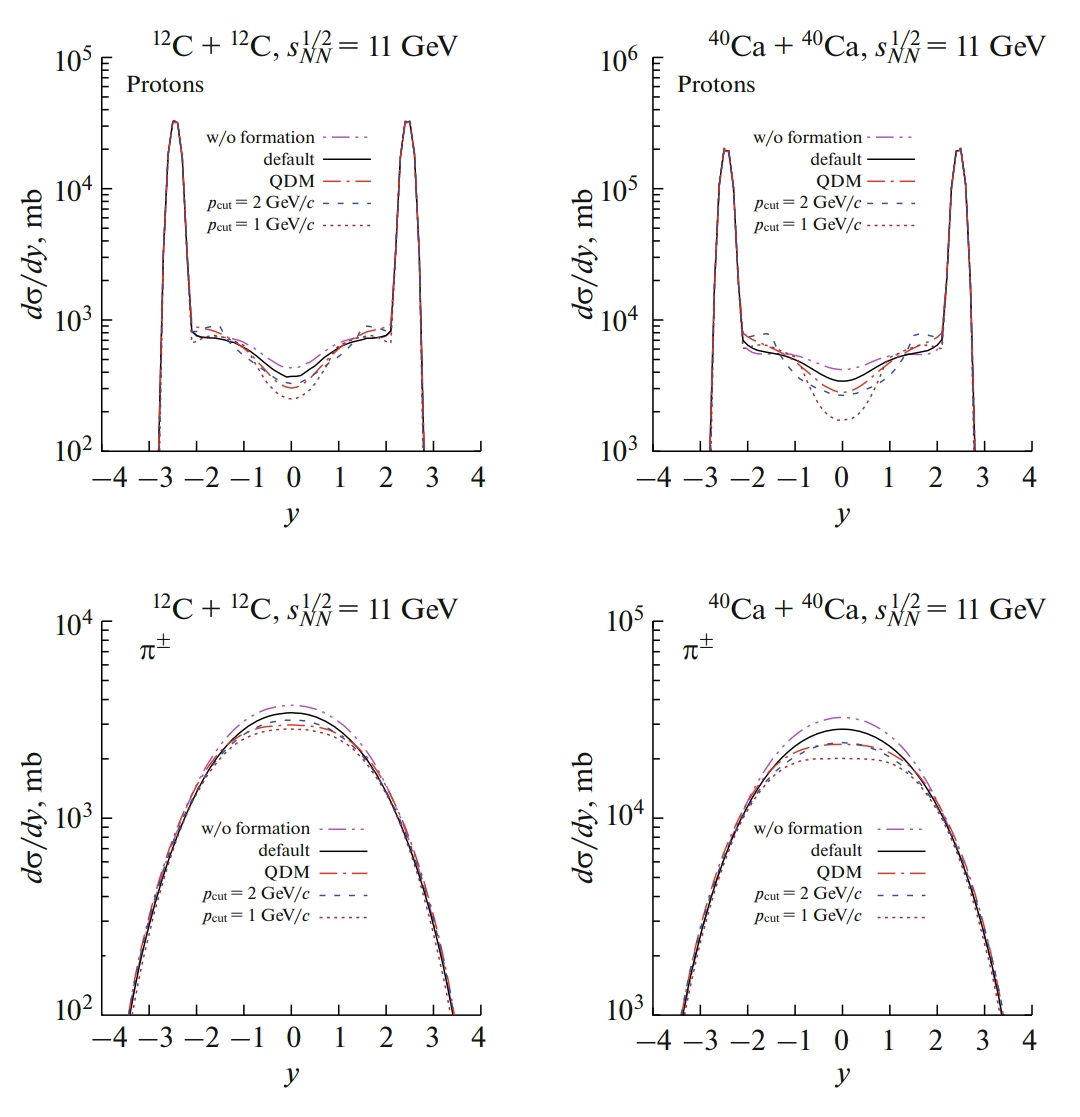
\includegraphics[scale=0.209]{ABRAMOV_Fig.36.jpg}
\caption{Rapidity spectra of protons and charged pions in $^{12}C-{^{12}C}$ and $^{40}Ca-{^{40}Ca}$ collisions.}
\label{ABRAMOV_Paper_Fig.36}
\end{subfigure}
\par
\hfill
\begin{subfigure}[h]{0.49\textwidth}
\centering
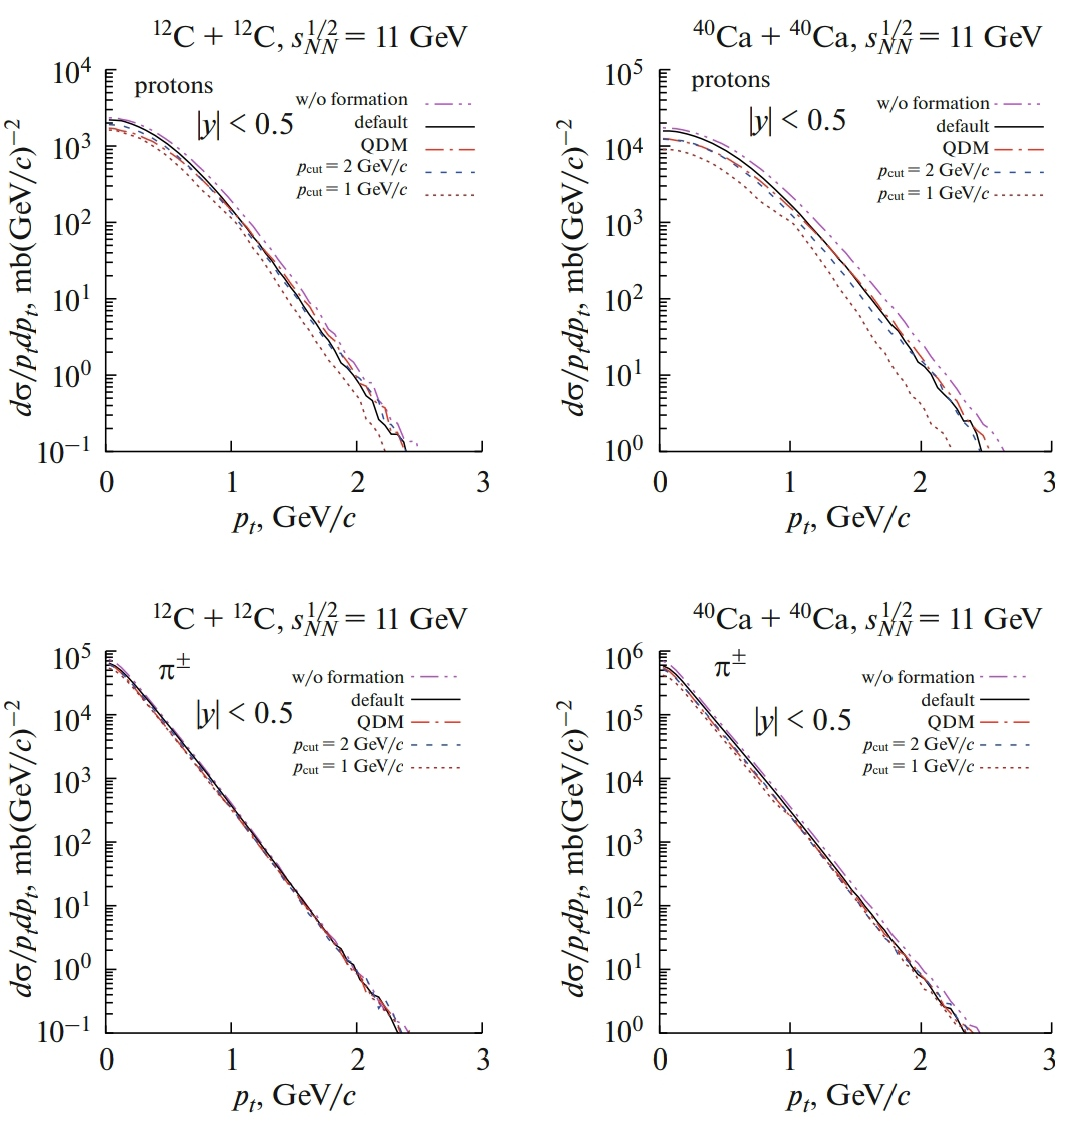
\includegraphics[scale=0.209]{ABRAMOV_Fig.37.jpg}
\caption{Transverse momentum spectra of protons and charged pions in $^{12}C-{^{12}C}$ and $^{40}Ca-{^{40}Ca}$ collisions.}
\label{ABRAMOV_Paper_Fig.37}
\end{subfigure}
\caption{Rapidity and transverse momentum spectra of protons and charged pions in $^{12}C-{^{12}C}$ and $^{40}Ca-{^{40}Ca}$ collisions.}
\label{ABRAMOV_Paper_Fig.36 and Fig.37}
\end{figure}

\begin{figure*}[h]
\centering
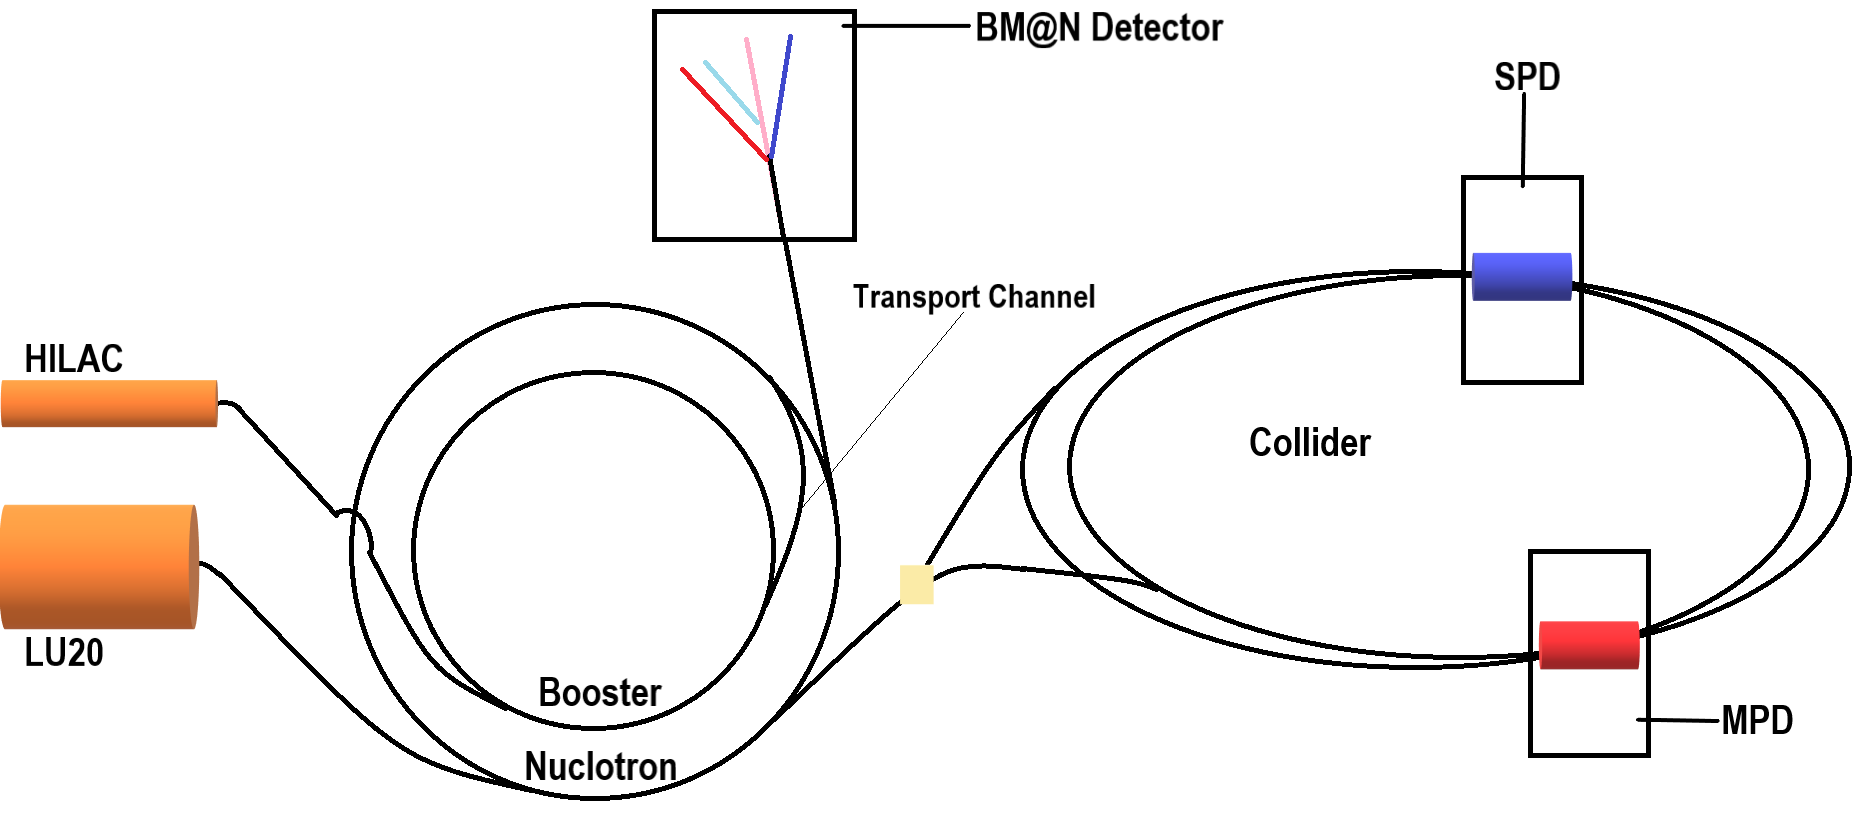
\includegraphics[scale=0.3]{NICA_Collider.png}
\caption{Schematic view of NICA complex.}
\label{Schematic view of NICA complex.}
\end{figure*}
 
  Once the NICA collider will be operational, scientists will be able to create a special state of matter in laboratory which existed for very short interval of time (\~20$\mu$ sec) just after the big bang. This special state is called as QGP (Quark Gluon Plasma) and it filled the entire universe shortly after the big bang.

The main parts of NICA facility consists of two independent injector complex (injector for light ions, and injector for heavy ions-KRION 6T), Light Ion Linear Accelerator (LU20) for accelerating light ions like protons ($H^{+}$), deutrons, and $\alpha$-particles upto 5 MeV of K.E, then Heavy Ion Linear Accelerator (HILAC) to accelerate heavy ions upto Au to a maximum K.E of 3.2 MeV/n, then a Super Conducting (SC) Booster Synchrotron to create ultra high vacuum and to provide complete stripping of heavy ions, then a SC Heavy Ion Synchrotron Nuclotron to accelerate both light and heavy ions to required beam energy \cite{kekelidze2017nica}. The accelerated beams will collide at two different locations where MPD detector and SPD detector are being built. The schematic view of NICA complex is shown in Fig.\ref{Schematic view of NICA complex.}.


% However, for this work, physics simulations were done on NICA-SPD setup using SPDroot to study different charged particles spectra and hence this paper is limited only to the working of SPD. The SPD setup has been explained in more detail in section \ref{SPD DETECTOR}.


% Heavy Ion collisions of $^{40}Ca-{^{40}Ca}$ and $^{12}C-{^{12}C}$ at $\sqrt{s}=11 AGeV$ were performed using SMASH (Simulating Many Accelerated Strongly-interacting Hadrons) event generator, then rapidity (y), transverse momentum (pT), and total momentum (p) spectra of charged pions, kaons, and protons were analysed at generator stage. Using SPDroot, same collisions were performed (taking all parameters same), and then the same plots were obtained at detector stage also. The goal was to check the performance of tracking systems - TOF \& ST, for charged pion, kaon, and proton identification. For same, the precision graph was obtained from momentum spectra of each charged particle mentioned above and then precision was estimated. It must be noted that $\pi^{+}$ and $\pi^{-}$ were considered together as pions, and similar assumptions were taken for kaons, and protons. Also, at first stage of NICA-SPD, there will be no calorimeters and hence only charged particles were considered at detector stage.

\section{SPD DETECTOR}
\label{SPD DETECTOR}
The Spin Physics Detector is a $4\pi$ universal detector being designed to study the properties of stable particles like nucleons, $\pi^{\pm}, k^{\pm}, e^{\pm}, \mu^{\pm}$, and photons by colliding polarized beams of p-p or d-d upto 27 GeV of collision energy to study the particle spin physics \cite{guskov2021spin, arbuzov2021physics, kekelidze2017feasibility}.
\begin{figure*}[h]
\centering
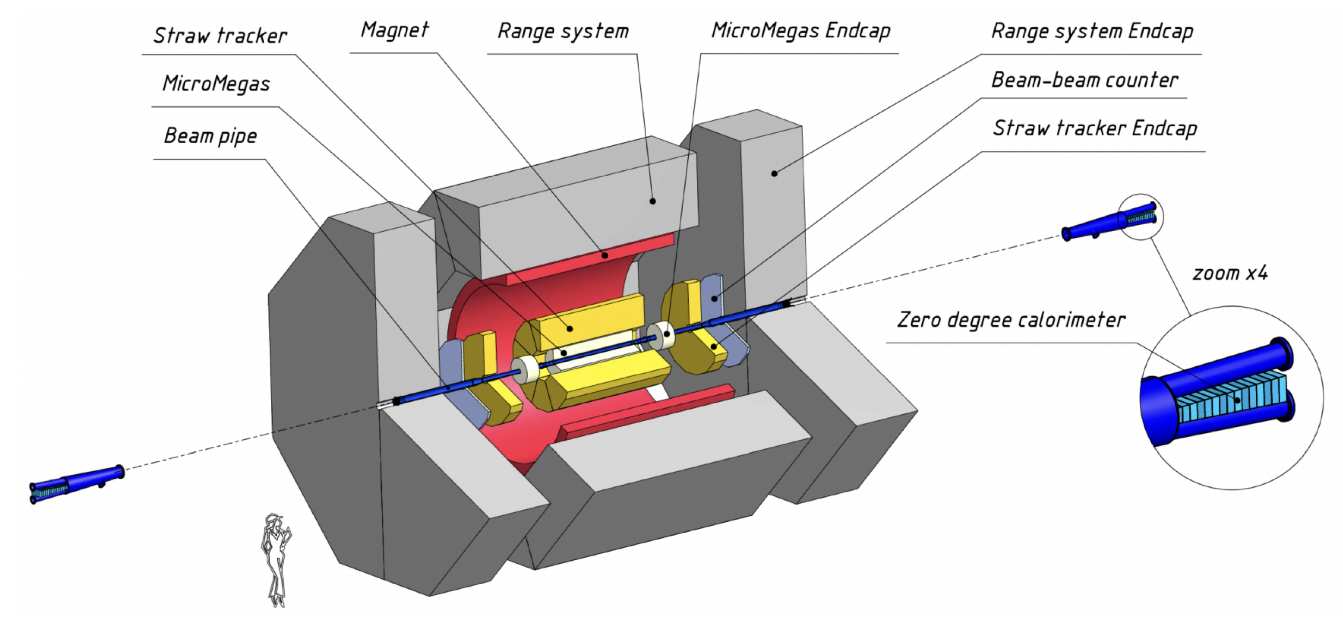
\includegraphics[scale=0.4]{Layout of the SPD setup proposed for first stage at NICA-SPD.png}
\caption{Layout of the SPD setup proposed for first stage at NICA-SPD.}
\label{Layout of the SPD setup proposed for first stage at NICA-SPD.}
\end{figure*}
However, at first stage of NICA-SPD, the expected collision energy will be around 10 GeV, and later on after first upgrade, it is expected to reach upto 27 GeV. The general layout depicting isometric projection of SPD setup is shown in Fig.\ref{Layout of the SPD setup proposed for first stage at NICA-SPD.}. The main parts involved in advanced tracking and particle identification capabilities have been shown. (i) The beam pipe passes through the center of the detector, carries the accelerated beams of ions. (ii) The MicroMegas detector is to improves the momentum resolution and tracking efficiency of the tracking system. (iii) The Straw Tracker (ST) detector is for the reconstruction of the primary and secondary particle tracks, and also to calculate momentum of the particle with high precision. (iv) The Time Of Flight (TOF) detector, is a part of Particle IDentification (PID) system, and is used for identification of particles like $\pi$, k, and p with long trajectories. (v) The magnet system shown by red color provides $1T$ of magnetic field along the beam axis. This setup is limited to first stage of SPD operation, and will be considered only for the identification of stable charged particles. Uncharged particles like $n^{0}$, photons will be detected at later stages. The main parts of SPD first stage have been explained in detail below.


\subsection{CENTRAL TRACKER}
The innermost detector of SPD consists of a MicroMegas-based Central Tracker (MCT). Its purpose is to identify the primary vertex coordinate and to improve momentum resolution and tracking efficiency of the main tracking system. It is based on MicroMegas (Micro Mesh Gaseous Structure) technology and detects charged particle by amplifying the charges produced due to ionization of the gas molecules present in detector volume. When an ionizing particle track passes through detector volume, it ionizes the gas molecules and creates few hundreds of $e^{-}$-ion pair. Electrons are accelerated opposite to the direction of applied electric field of $600 V/cm$ in ionization gap, while ions are attracted towards cathode. When the $e^{-}$ crosses micromesh, it faces intense electric field ($>30KV/cm$) and gains enough energy to ionize other gas molecules in its path. During this process an avalanche of $e^{-}$-ion pair is produced ($1e^{-}$ produces $10^4$ $e^{-}$-ion pairs) which is significant to create an electronic signal which is read out by readout electrodes.   

\subsection{STRAW TRACKER}
\label{STRAW TRACKER}
ST is mainly for the reconstruction of primary and secondary particle tracks but also participates in identification of $\pi$, k, and p (in low momentum region) via energy deposition $(dE/dX)$ measurement \cite{kekelidze2013project}. It is also used to measure the total momentum of particles which passes through it. It consists of two major parts - barrel (covers radius from 270 to 850 mm) and two end-caps. The barrel is divided into 8 modules enclosed in a carbon fiber capsule. Each module has 30 double layers of straw tubes (dia 1cm) which runs parallel (long straw tubes) and perpendicular (short straw tubes) to the beam axis and contains 1500 and 6000 parallel and perpendicular straw tubes respectively. Straw tubes are made of polyethylene terephthalate and outer surface is coated with very thin layer of Cu and Au. Carbon capsule is meant to protect the outer surface of these tubes from humidity. One side and two opposite ends of capsule are provided with small holes where end plugs are fixed. FEE are connected to these end plugs to read the detector signal. Any particle which passes through the long straws will send detector signal to both opposite ends while a particle passing through short straw will send detector signal to any one side of capsule where FEE is attached. Thus, long straws will be read from two opposite ends while short straws will be read from one side. The end-caps of ST are divided into 3 modules and each module has 4 hexadecimal cameras (U, V, X, Y) to record the four coordinates of any physical quantity like four-momentum \cite{abazov2021conceptual}. The FEE to be used can be similar to the one used at NA64 experiment (for the search of dark matter) \cite{volkov2019straw}, or DUNE experiment (to detect and study properties of neutrino) \cite{acciarri2016long}.

\subsection{TIME OF FLIGHT DETECTOR}
TOF detector is the part of PID system. It provides identification of $\pi$, k, and p (in broad momentum region) which has enough long trajectories to reach the PID system. Along with this, it also measures the momentum of particles with high precision. It often happens that the particles passing through ST decays into other stable particles, or undergo mutual interaction, or interact with the detector material and gets converted to some another particle. In this case the parent particle remains undetected by TOF. The energy loss data registered by ST is used together with the data from PID for correct identification of particle tracks. The TOF also distinguishes charged particles (mainly $\pi$ and k) on the basis of their masses in the momentum region of upto few GeV. The major parts of TOF comprises of a barrel and two end-caps. For the first stage of NICA-SPD, two different designs of TOF have been proposed. First one is TOF based on multigap timing Resistive Plate Chambers (mRPC), which will consist 220 rectangular plate chambers (160 for the barrel and 30 each for end-caps). Second one is based on Plastic Scintillator Tiles and will comprise 10.1K small scintillator tiles (7.4K for barrel and 1.4K for each end-caps). Scintillator has a property of emitting light in visible region when an ionizing radiation passes through it. So, in this design when a particle passes through TOF, scintillated photons are produced which are detected by four Si Photo Multipliers (SiPMs) present at each sensor board attached at two extreme ends of scintillator tile.

\section{EVENT GENERATION}

\begin{figure*}[h]
\centering
\begin{subfigure}[h]{0.49\textwidth}
\centering
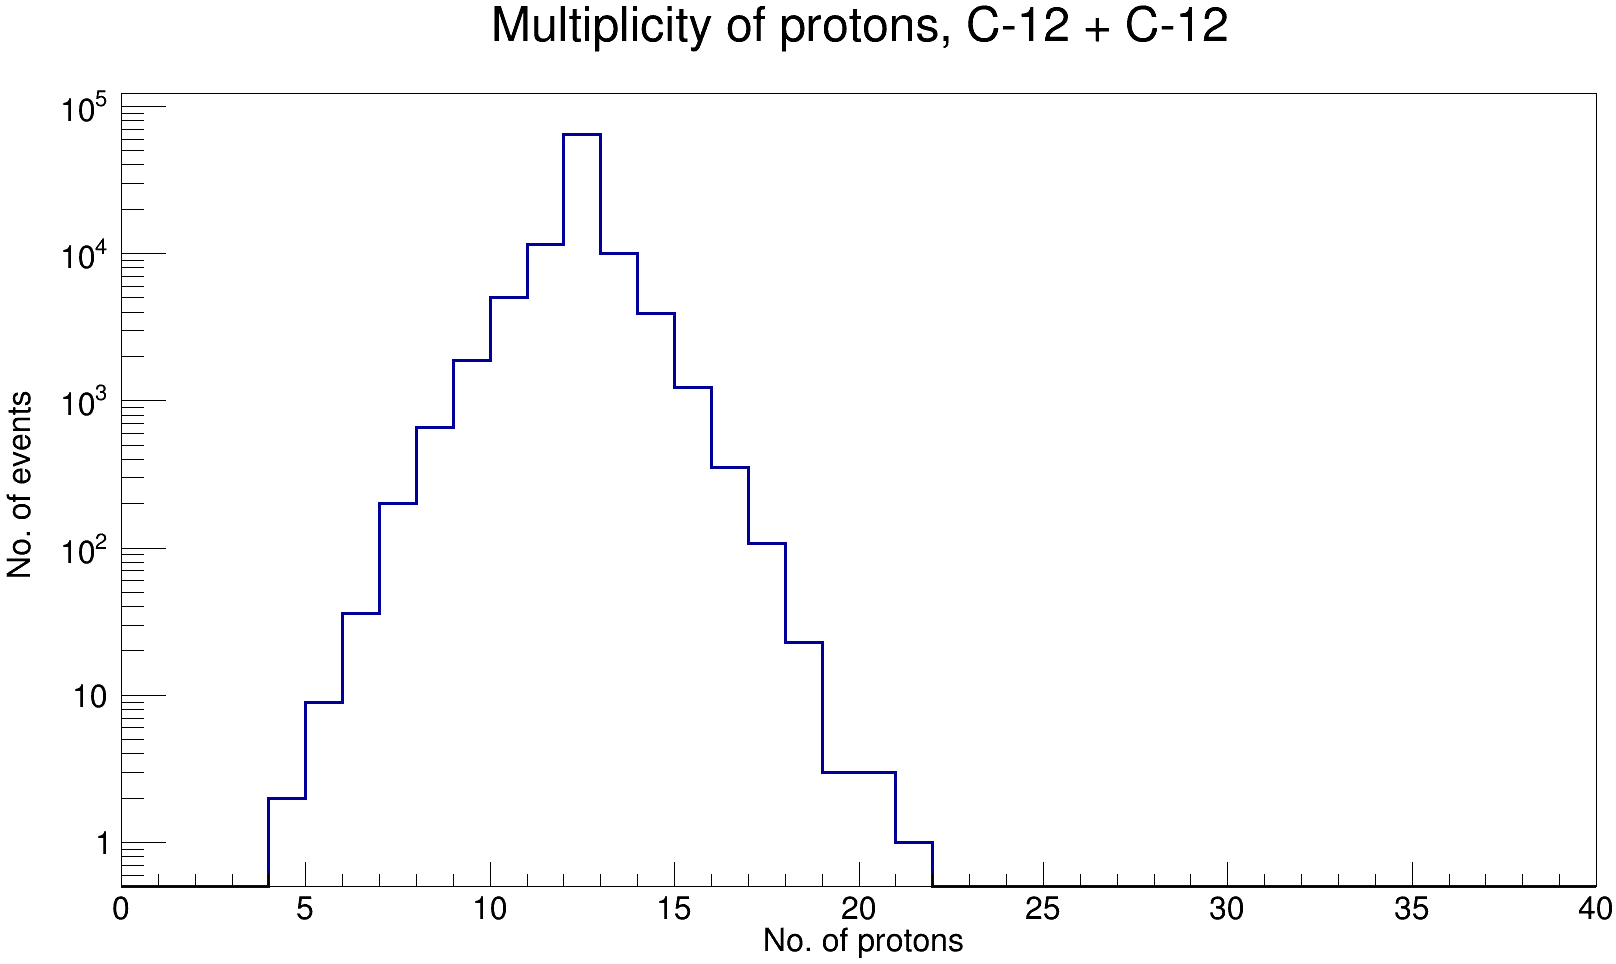
\includegraphics[scale=0.14]{ProtonMultiplicity_C12.png}
\caption{Multiplicity of $p^{\pm}$.}
\label{Multiplicity of protons C12.}
\end{subfigure}
\hfill
\vspace*{0.8cm}
\begin{subfigure}[h]{0.49\textwidth}
\centering
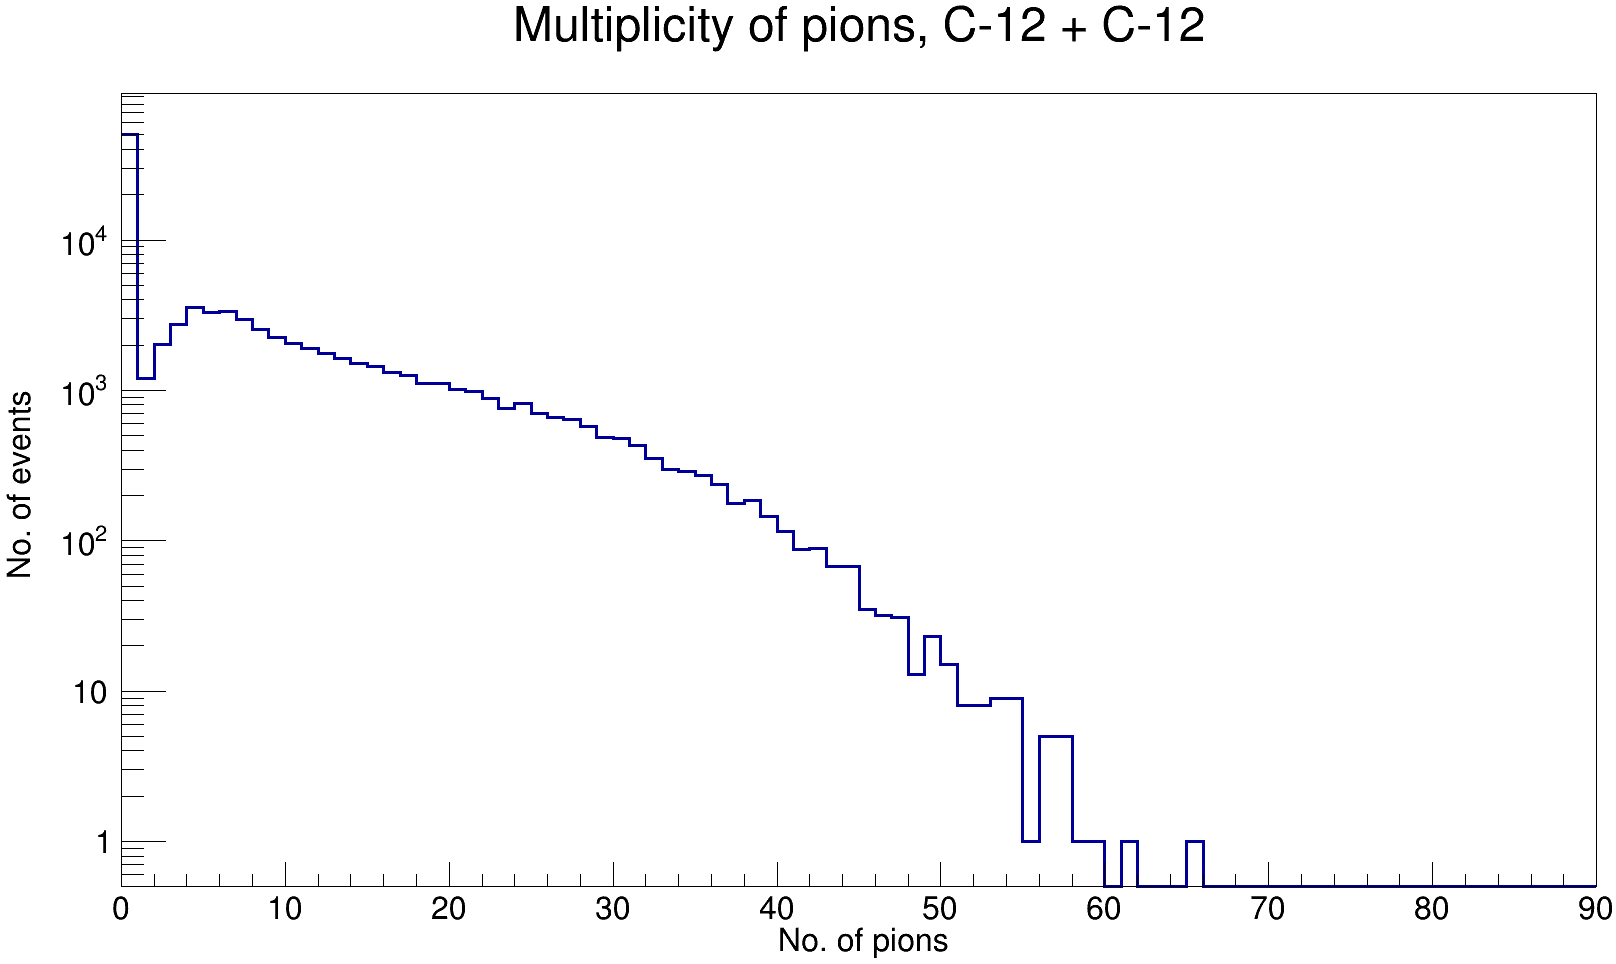
\includegraphics[scale=0.14]{PionMultiplicity_C12.png}
\caption{Multiplicity of $\pi^{\pm}$.}
\label{Multiplicity of pions C12.}
\end{subfigure}
\hfill
\begin{subfigure}[h]{0.49\textwidth}
\centering
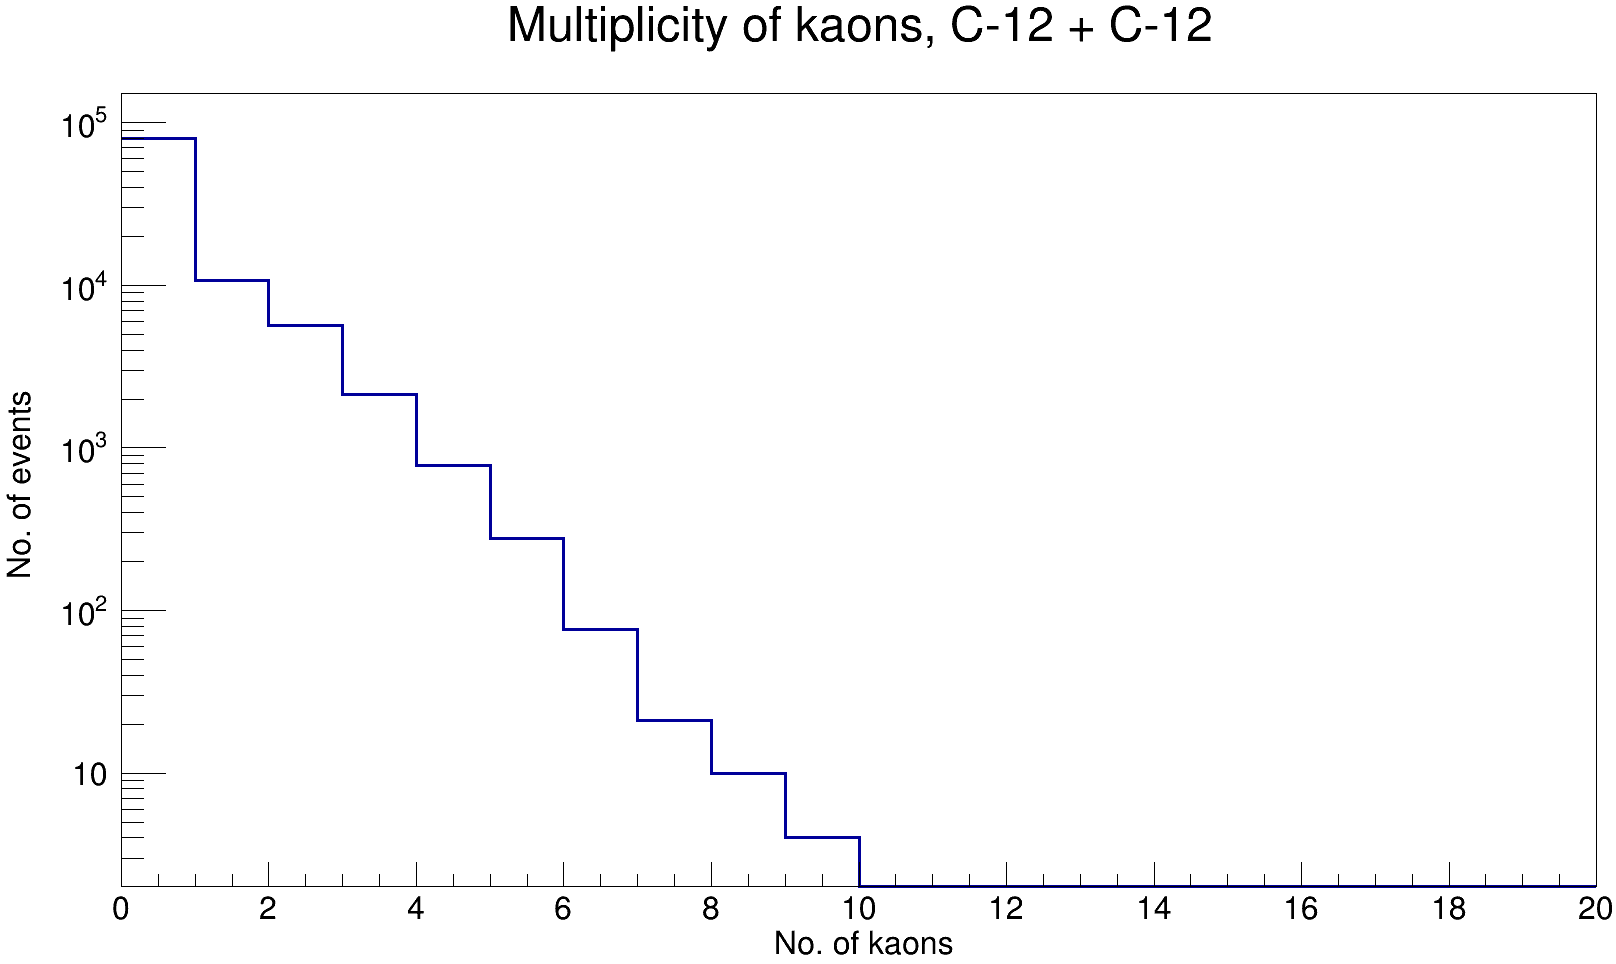
\includegraphics[scale=0.14]{KaonMultiplicity_C12.png}
\caption{Multiplicity of $k^{\pm}$.}
\label{Multiplicity of kaons C12.}
\end{subfigure}
\hfill
\begin{subfigure}[h]{0.49\textwidth}
\centering
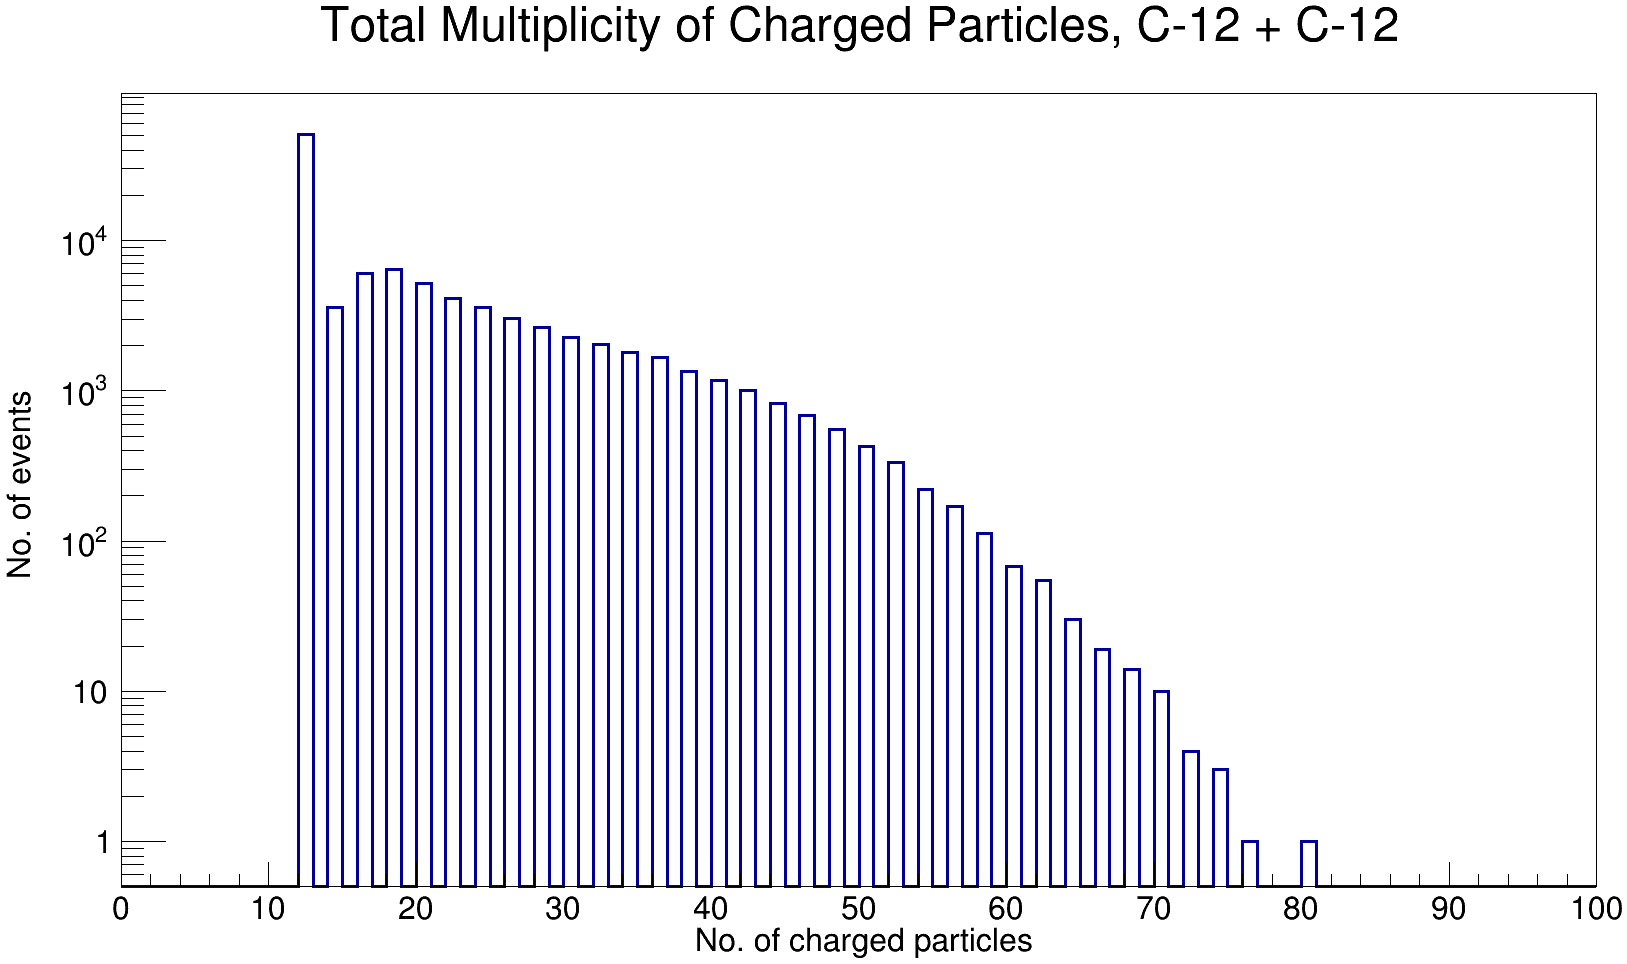
\includegraphics[scale=0.14]{GeneratorTotalMultiplicity_C12.png}
\caption{Total multiplicity of all charged particles.}
\label{Total multiplicity of all charged particles C12.}
\end{subfigure}
\caption{Multiplicity of charged particles considered separately (see (a), (b), (c)) and Total multiplicity considering all charged particles together (see (d)) in $^{12}C-{^{12}C}$ collision (Generator level).}
\label{Multiplicity of charged particles considered separately and Total multiplicity considering all charged particles together in C12-C12 collision (Generator stage).}
\end{figure*}

$^{12}C-{^{12}C}$ and $^{40}Ca-{^{40}Ca}$ heavy ion collisions at $\sqrt{s}=11$~AGeV with maximum impact parameter set to 8~fm for C-C and 11~fm for Ca-Ca were simulated using SMASH. The fermi motion was assumed to be ``frozen'' and 100K events were generated for each heavy ion collision. The SMASH input file for C-C collision is shown below. 
\begin{verbatim}
*********** SMASH INPUT ************

config.yaml file for C-C collision.

Logging:
    default: INFO

General:
    Modus:          Collider
    Time_Step_Mode: Fixed
    Delta_Time:     0.1
    End_Time:       200.0
    Randomseed:     -1
    Nevents:        100000

Output:
    Output_Interval: 10.0
    Particles:
        Format:       ["Oscar2013"]

Modi:
    Collider:
        Projectile:
            Particles: {2212: 6, 2112: 6}
        Target:
            Particles: {2212: 6, 2112: 6}
            
        Sqrtsnn: 11.0
        
        Impact:
            Sample: "quadratic"
            Range: [0.0, 8.0]

        Fermi_Motion: "frozen"
    
\end{verbatim}

Multiplicity of generated final charged particles are shown by Fig.\ref{Multiplicity of charged particles considered separately and Total multiplicity considering all charged particles together in C12-C12 collision (Generator stage).} \& \ref{Multiplicity of charged particles considered separately and Total multiplicity considering all charged particles together in Ca40-Ca40 collision (Generator stage).} for C-C and Ca-Ca  collisions while kinematic distributions which include rapidity (y), total momentum (p), and transverse momentum (pT) distributions of protons, pions and kaons are shown by Fig.\ref{Rapidity distribution of charged particles in C12-C12 and Ca40-Ca40 collision.}, \ref{Total momentum distribution of protons, pions, and kaons at generator level in C12-C12 and Ca-Ca40 collision.}, \& \ref{Transverse momentum distribution of protons, pions, and kaons at generator level in C12-C12 and Ca-Ca40 collision.} for both C-C and Ca-Ca  collisions respectively. It was observed in each heavy ion collision, the charged tracks were mainly of $p^{\pm}, \pi^{\pm},$ \& $k^{\pm}$ and very few numbers of sigmas, cascades, and omegas. Hence, for C-C collisions, the total multiplicity of all charged particles, shown by Fig.\ref{Total multiplicity of all charged particles C12.} is the resultant of individual charged particle multiplicities shown by Fig.\ref{Multiplicity of protons C12.}, \ref{Multiplicity of pions C12.}, \& \ref{Multiplicity of kaons C12.}. Out of 100K events of each collision, maximum events resulted in zero $\pi^{\pm}$ and $k^{\pm}$ production. In $p^{\pm}$ multiplicity, the peak was observed at 12, due to 12 protons in two colliding $^{12}C$+$^{12}C$ ions. Similarly, there is a huge peak observed at 12 in total multiplicity plot, due to 12 charged particles at the beginning of collision. The $p^{\pm}$ multiplicity has a gaussian shape, while $\pi^{\pm}$ and $k^{\pm}$ multiplicity plots can be fitted with the equation of straight line $y=mmx+c$ to some extent. 

Fig.\ref{Rapidity distribution of charged particles in C12-C12 collision.} and \ref{Rapidity distribution of charged particles in Ca40-Ca40 collision.} shows the y-spectra of $p^{\pm}, \pi^{\pm}, k^{\pm}$ in C-C and Ca-Ca collision. The two peaks of proton rapidity spectrum at $y=\pm2.5$ corresponds to the initial rapidity of protons at the beginning of collision. For pion and kaon rapidity spectra, the peak lies somewhere near $y=0$.

The generator level p and pT momentum spectra are obtained in midrapidity region ($|y|<0.5$), and are qualitatively similar to the one mentioned in paper Ref.\cite{abramov2021possible}.


\begin{figure*}[h]
\centering
\begin{subfigure}[h]{0.49\textwidth}
\centering
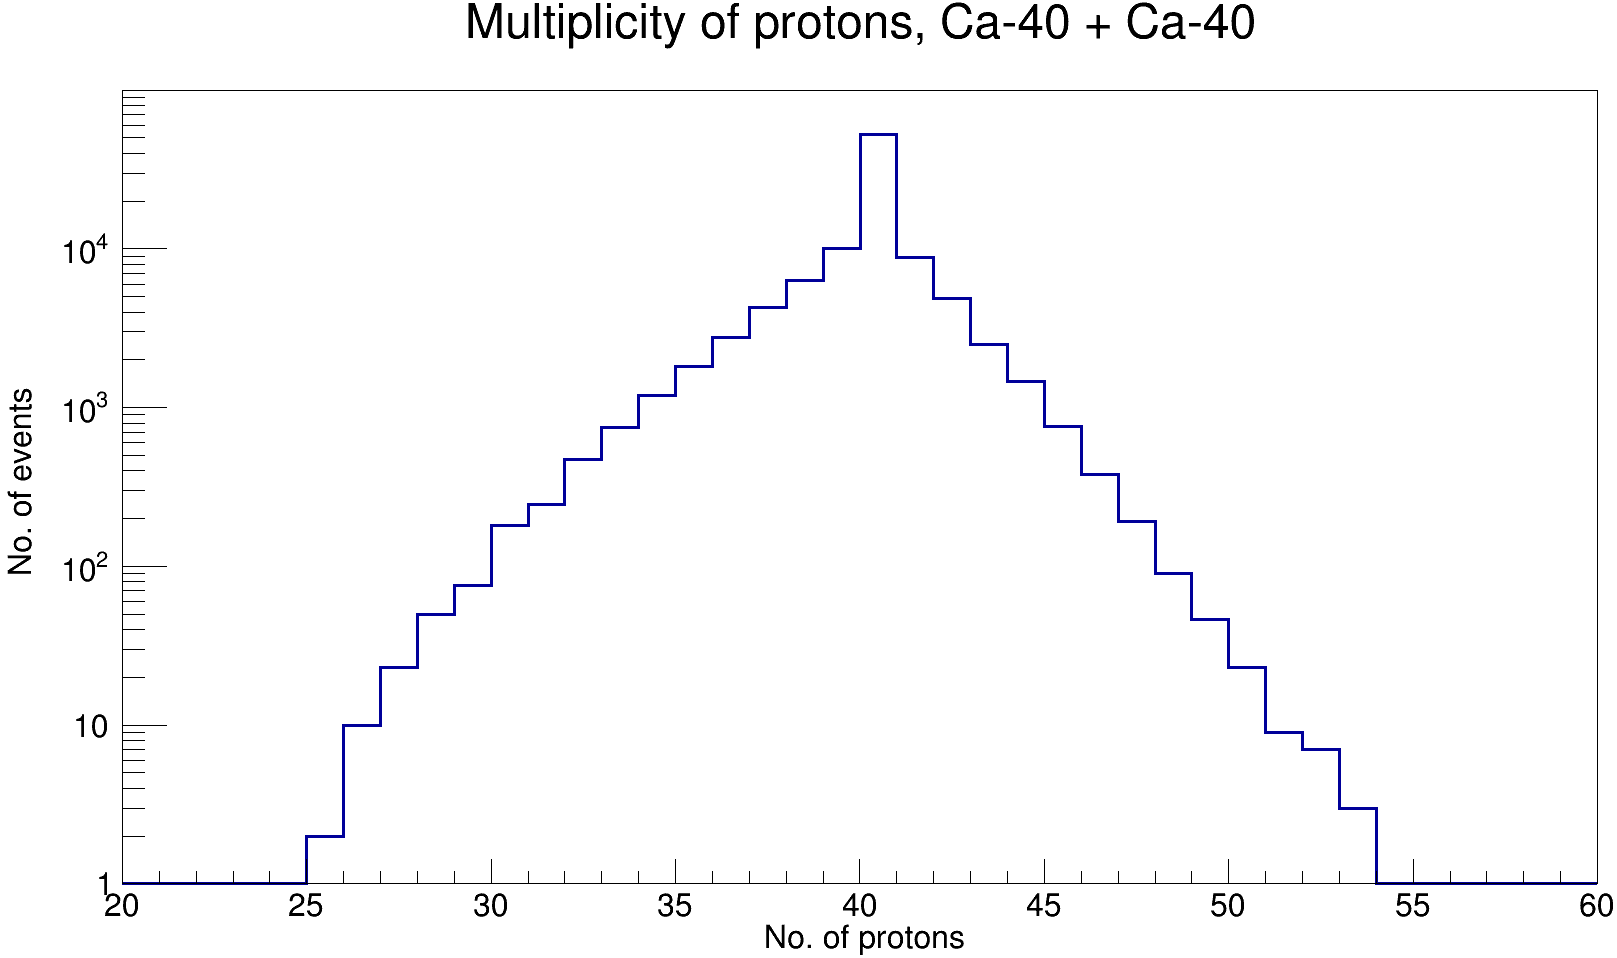
\includegraphics[scale=0.14]{ProtonMultiplicity_Ca.png}
\caption{Multiplicity of $p^{\pm}$.}
\label{Multiplicity of protons Ca40.}
\end{subfigure}
\hfill
\vspace*{1.5cm}
\begin{subfigure}[h]{0.49\textwidth}
\centering
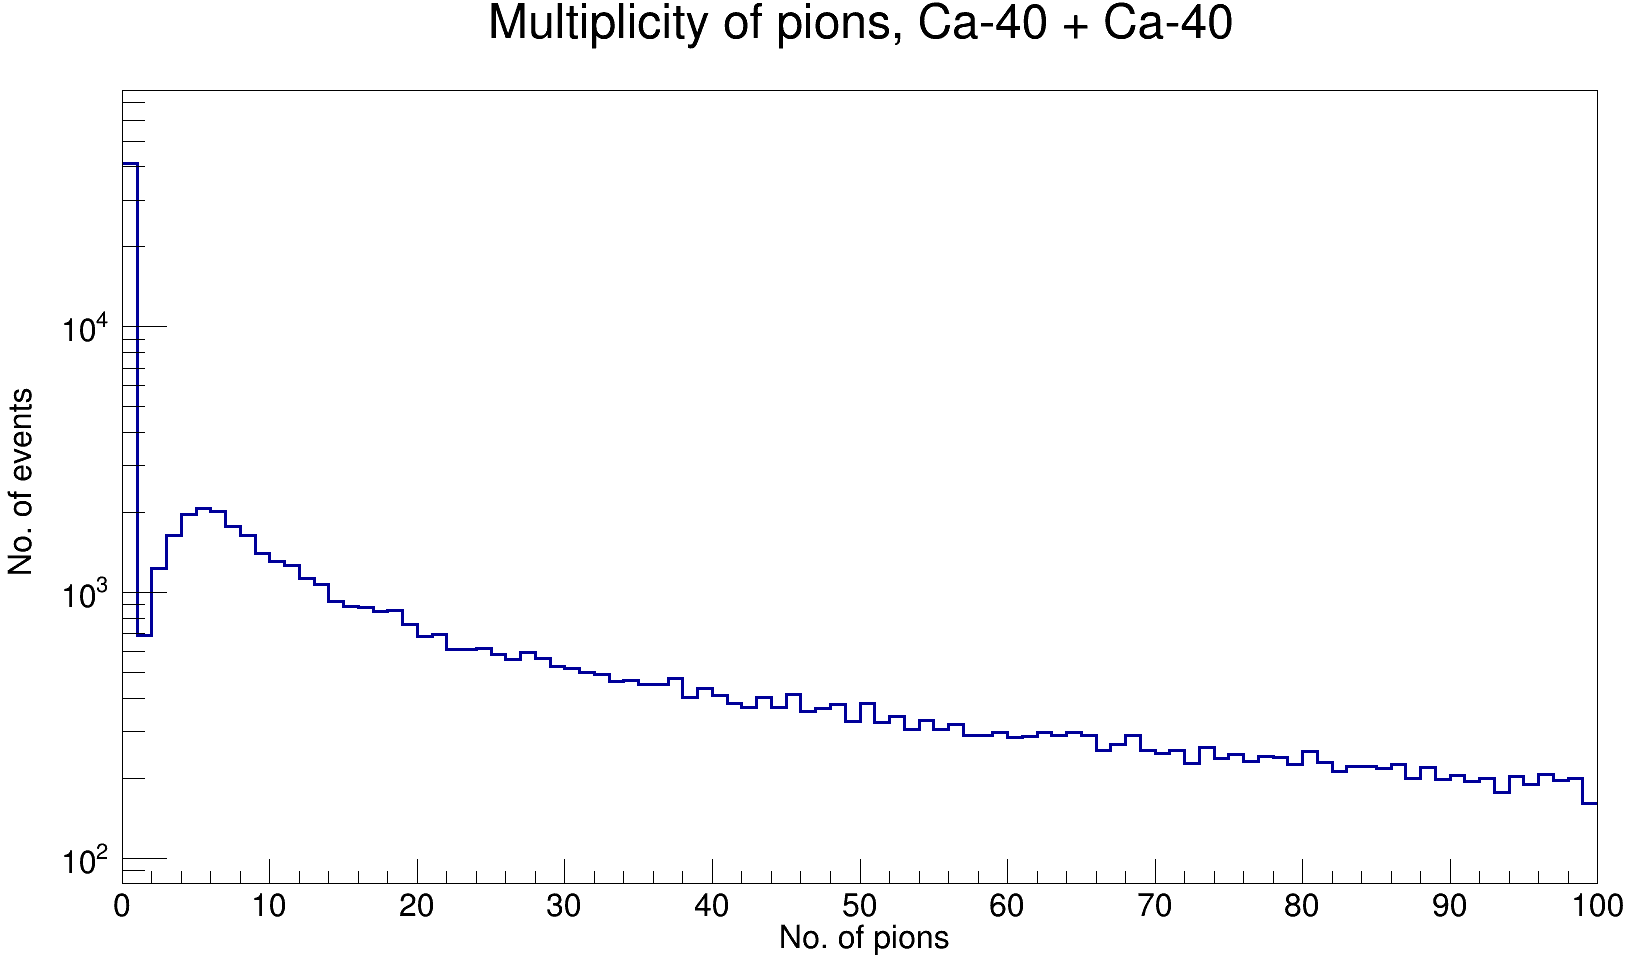
\includegraphics[scale=0.14]{PionMultiplicity_Ca.png}
\caption{Multiplicity of $\pi^{\pm}$.}
\label{Multiplicity of pions Ca40.}
\end{subfigure}
\hfill
\begin{subfigure}[h]{0.49\textwidth}
\centering
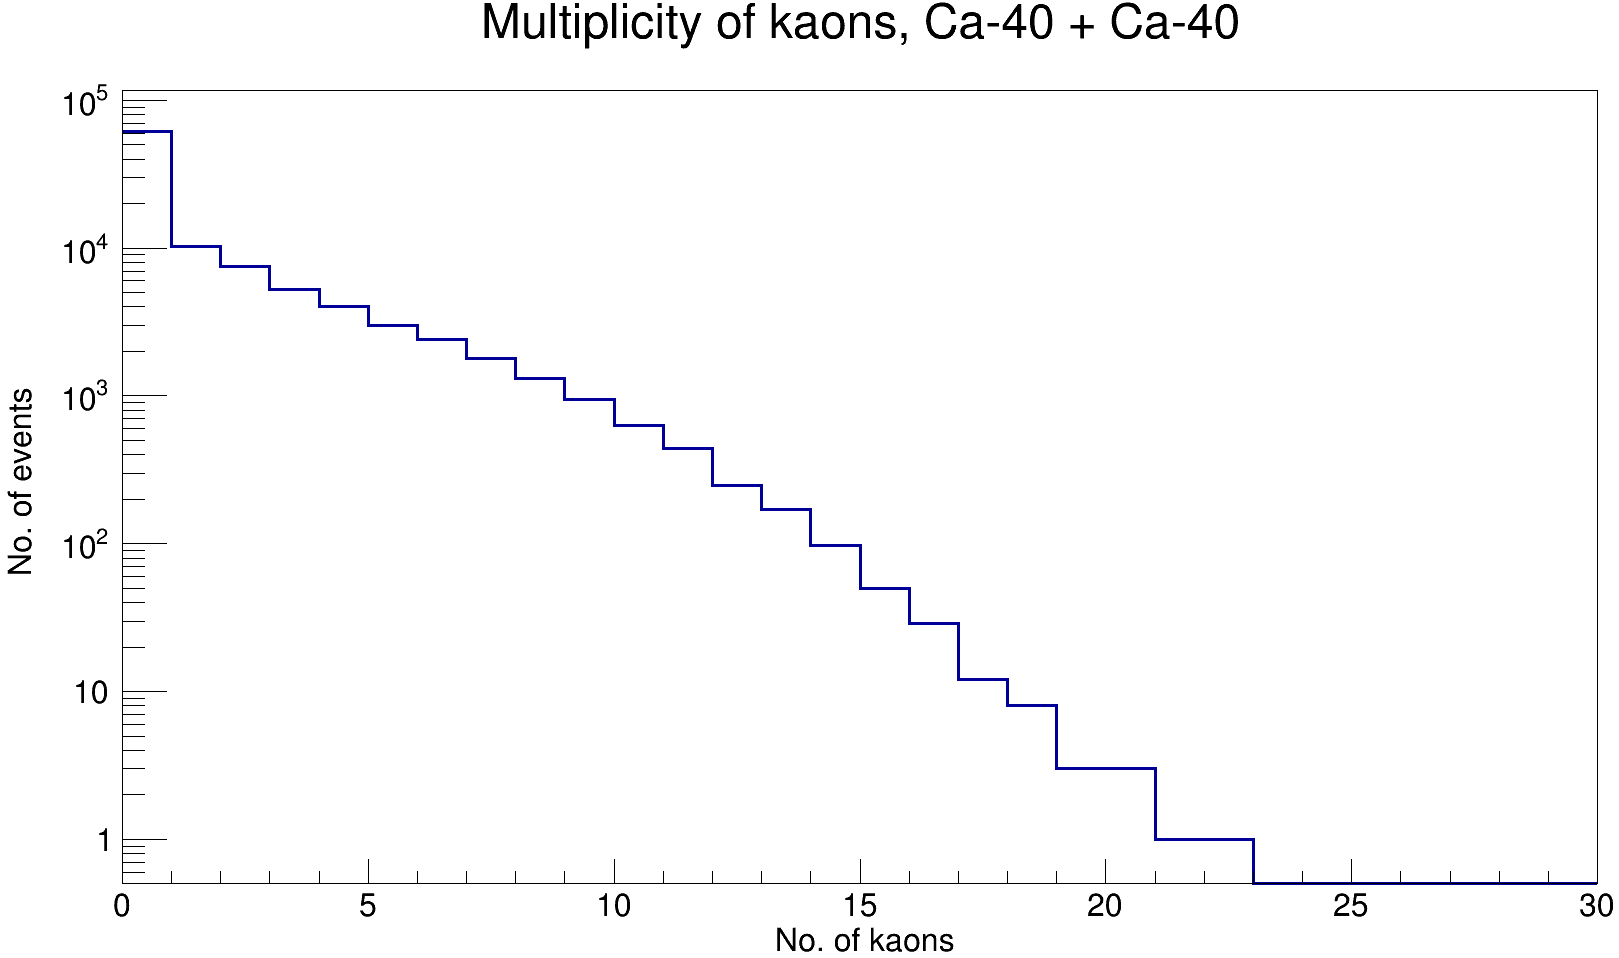
\includegraphics[scale=0.14]{KaonMultiplicity_Ca.png}
\caption{Multiplicity of $k^{\pm}$.}
\label{Multiplicity of kaons Ca40.}
\end{subfigure}
\hfill
\begin{subfigure}[h]{0.49\textwidth}
\centering
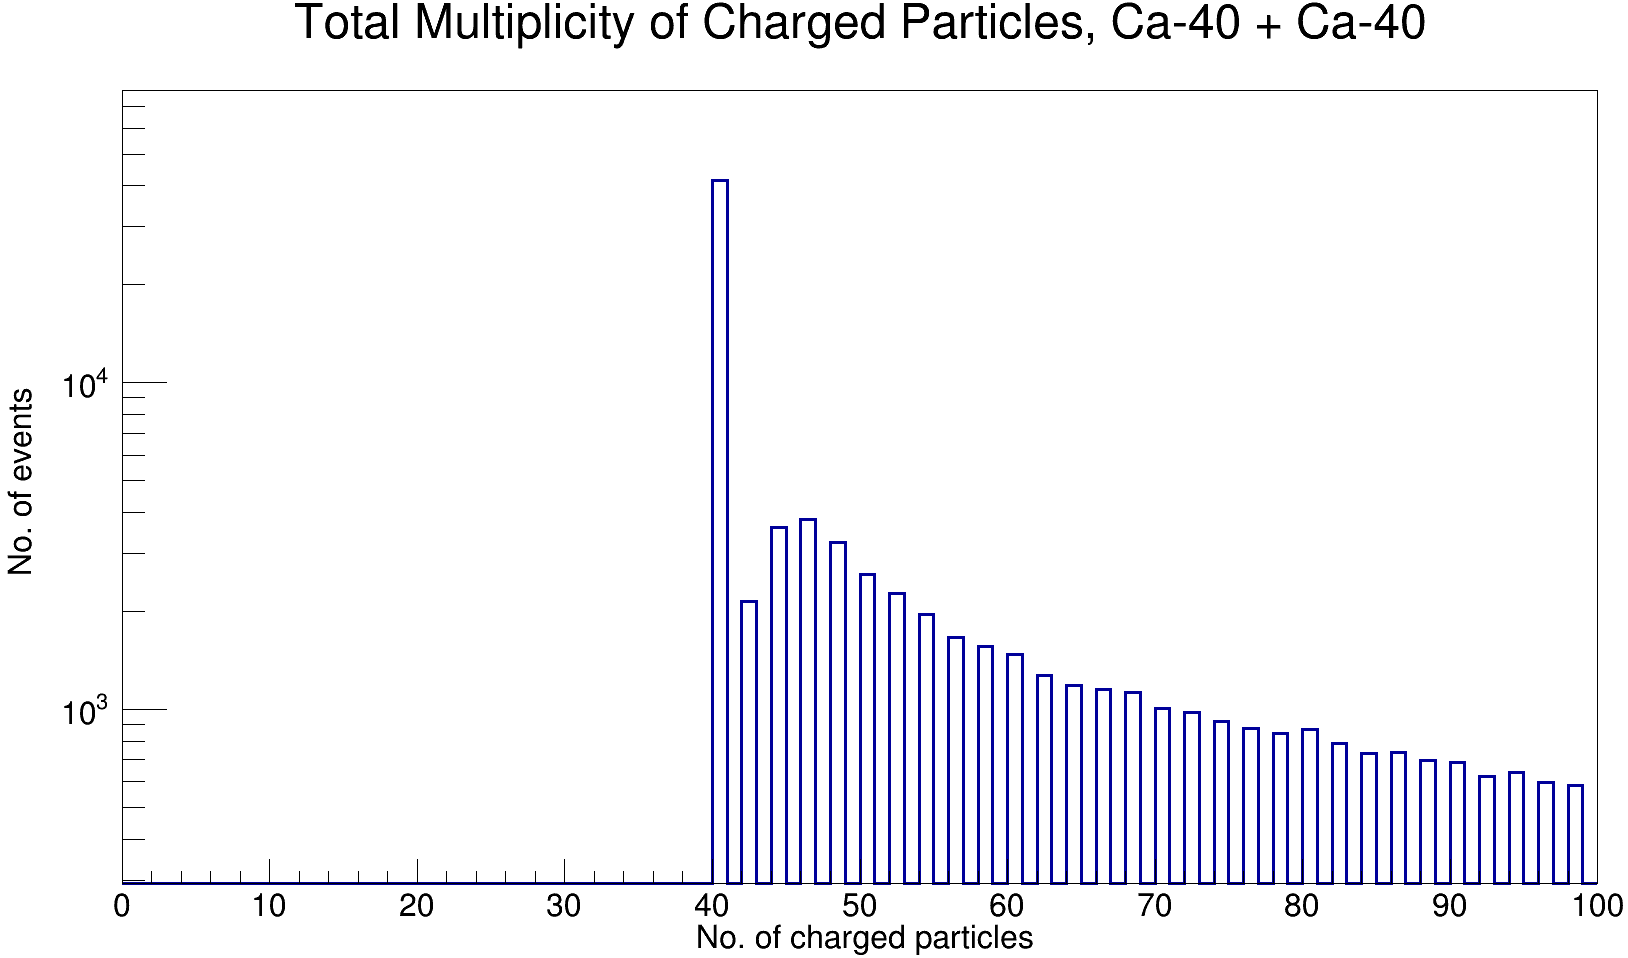
\includegraphics[scale=0.14]{GeneratorTotalMultiplicity_Ca40.png}
\caption{Total multiplicity of all charged particles.}
\label{Total multiplicity of all charged particles Ca40.}
\end{subfigure}
\caption{Multiplicity of charged particles considered separately (see (a), (b), (c)) and Total multiplicity considering all charged particles together (see (d)) in $^{40}Ca-{^{40}Ca}$ collision (Generator level).}
\label{Multiplicity of charged particles considered separately and Total multiplicity considering all charged particles together in Ca40-Ca40 collision (Generator stage).}
\end{figure*}


\begin{figure*}[h]
\centering
\begin{subfigure}[h]{0.49\textwidth}
\centering
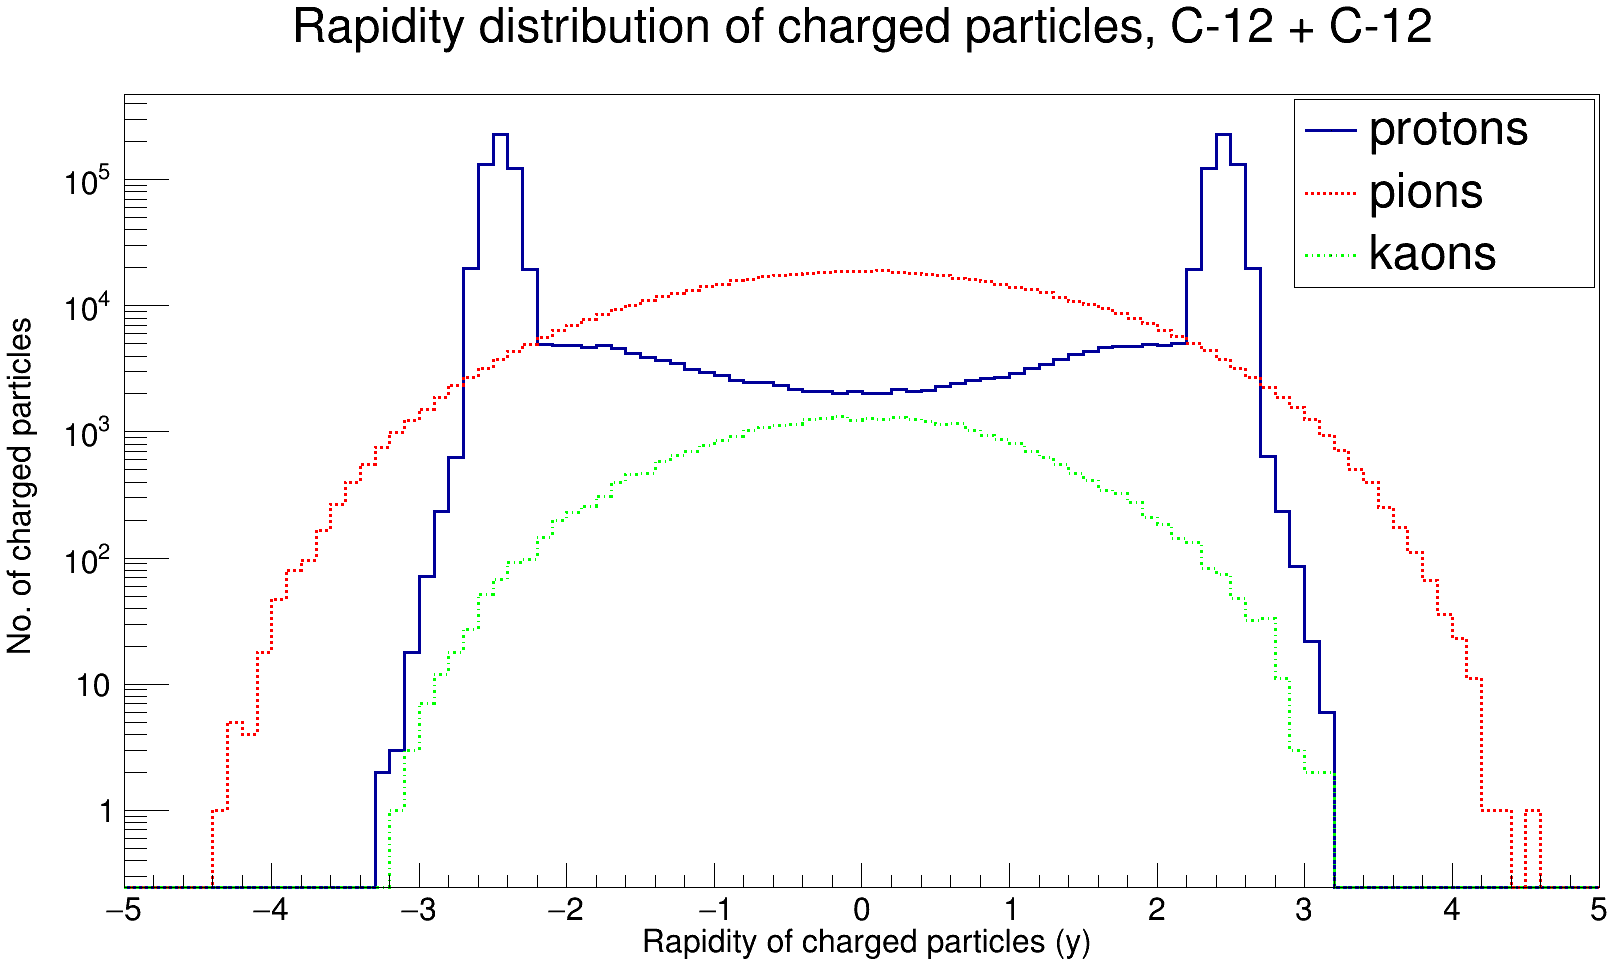
\includegraphics[scale=0.14]{RapidityC12.png}
\caption{Rapidity distribution of charged particles in $^{12}C-{^{12}C}$ collision.}
\label{Rapidity distribution of charged particles in C12-C12 collision.}
\end{subfigure}
\hfill
\begin{subfigure}[h]{0.49\textwidth}
\centering
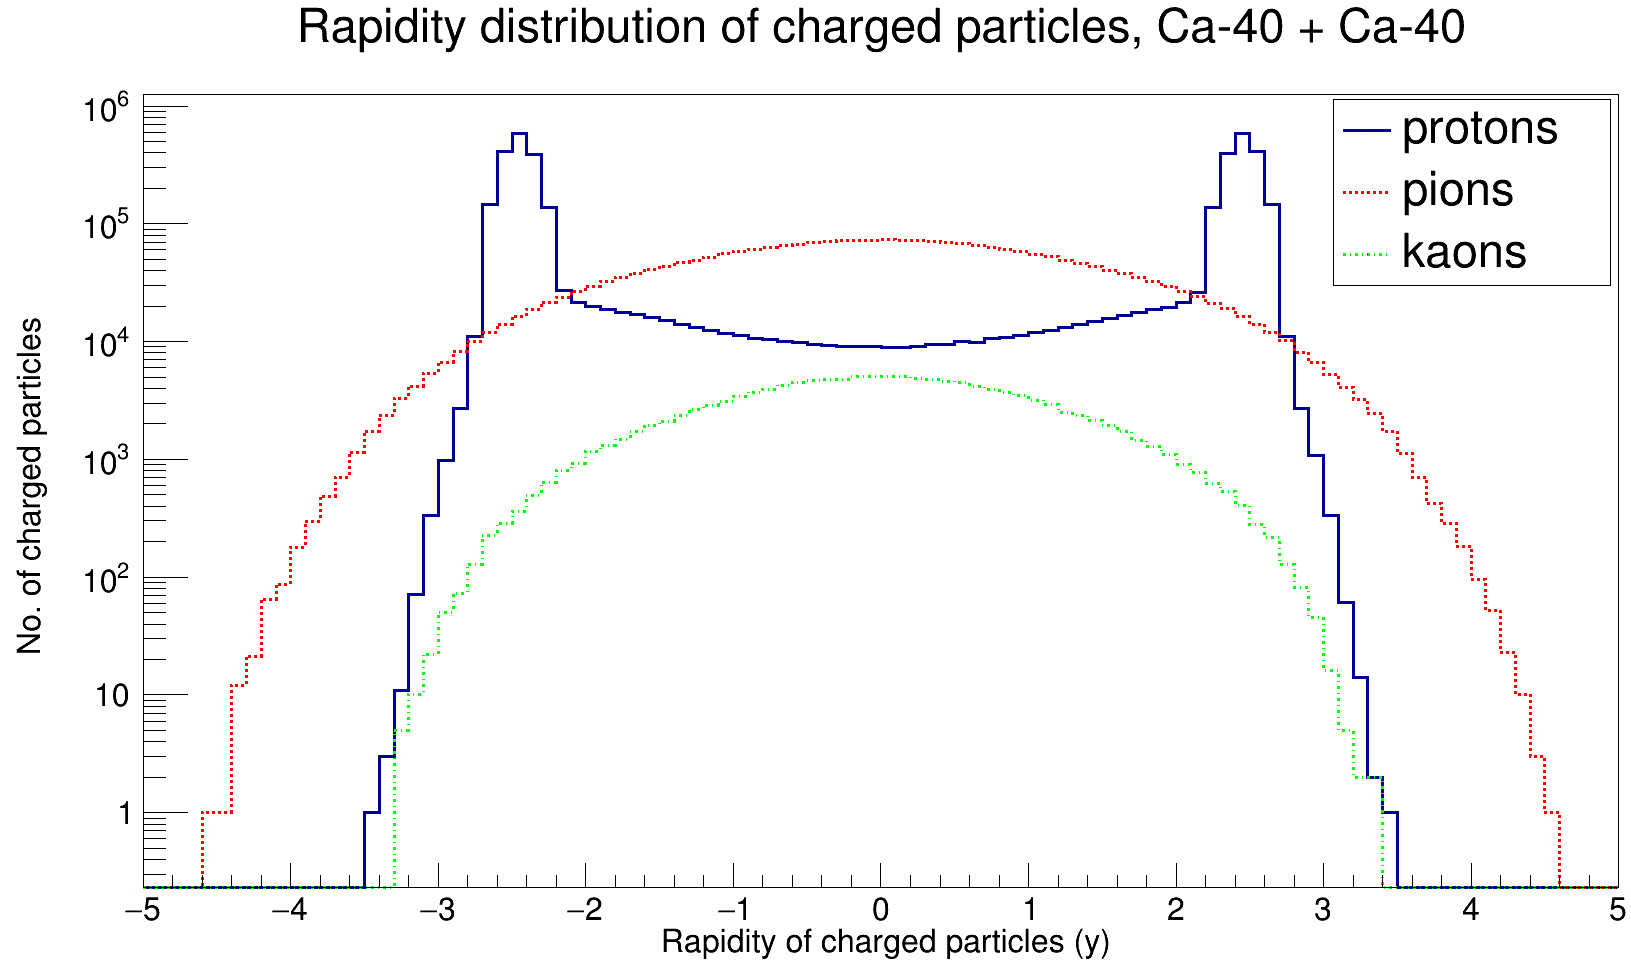
\includegraphics[scale=0.14]{RapidityCa40.png}
\caption{Rapidity distribution of charged particles in $^{40}Ca-{^{40}Ca}$ collision.}
\label{Rapidity distribution of charged particles in Ca40-Ca40 collision.}
\end{subfigure}
\caption{Rapidity distribution of charged particles in $^{12}C-{^{12}C}$ and $^{40}Ca-{^{40}Ca}$ collision.}
\label{Rapidity distribution of charged particles in C12-C12 and Ca40-Ca40 collision.}
\end{figure*}

%\clearpage


\begin{figure*}[h]
\centering
\begin{subfigure}[h]{0.49\textwidth}
\centering
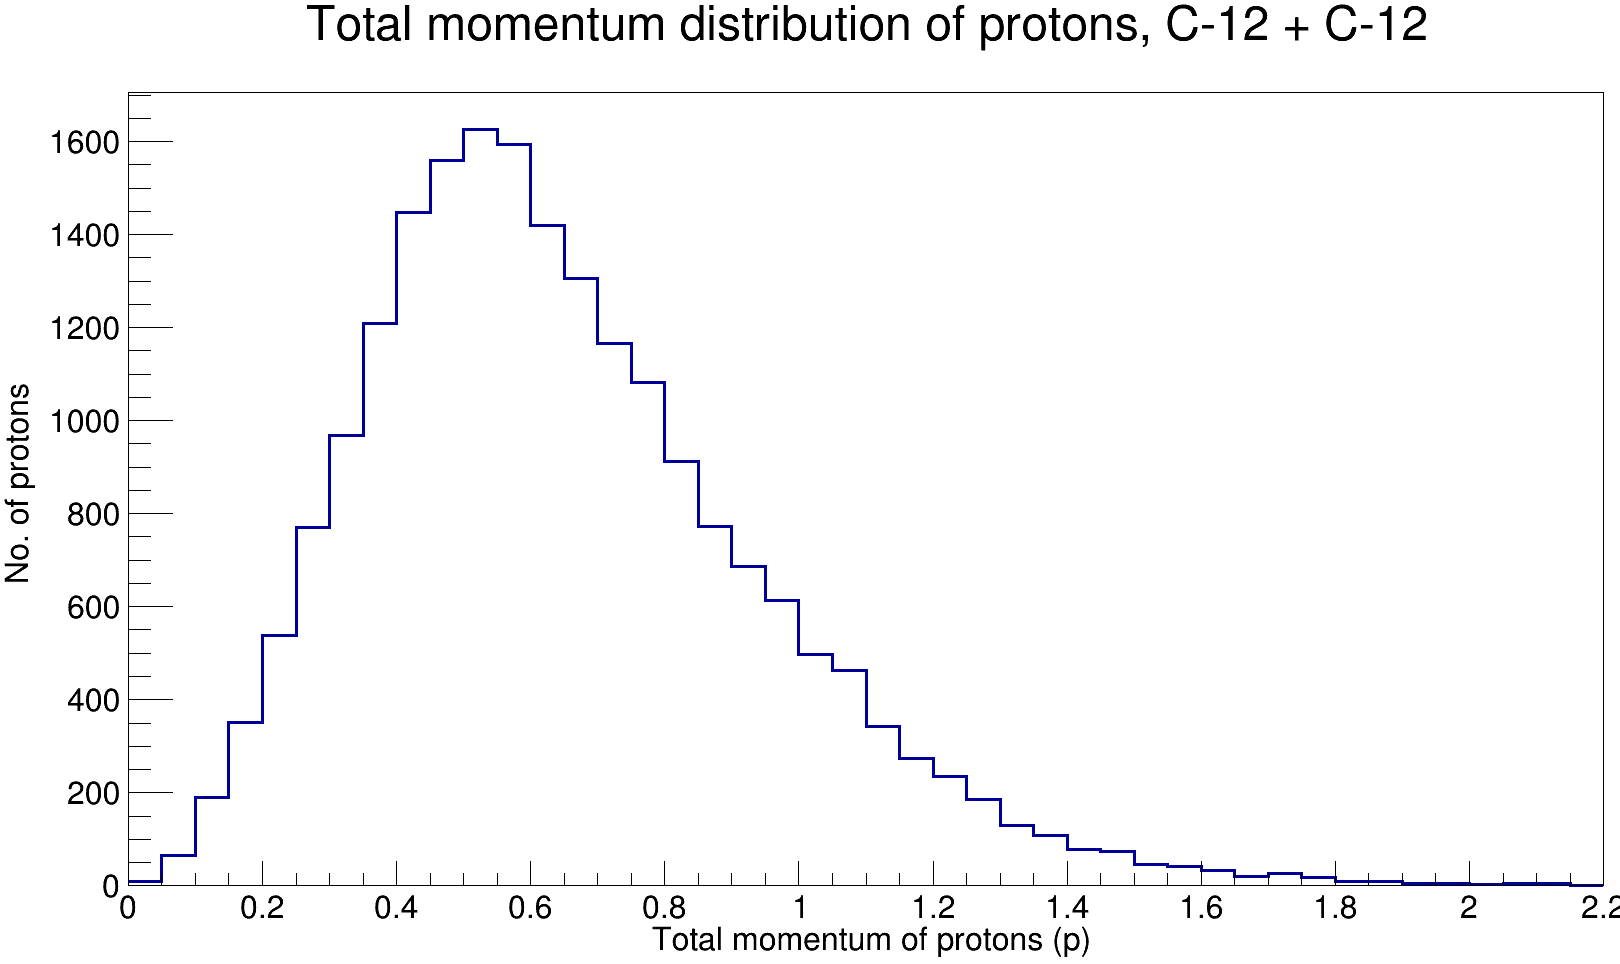
\includegraphics[scale=0.14]{pToT_protons_C12.png}
\caption{p distribution of $p^{\pm}$ in $^{12}C-{^{12}C}$ collision.}
\label{Generator - Total momentum distribution of protons C12.}
\end{subfigure}
\hfill
\vspace*{1cm}
\begin{subfigure}[h]{0.49\textwidth}
\centering
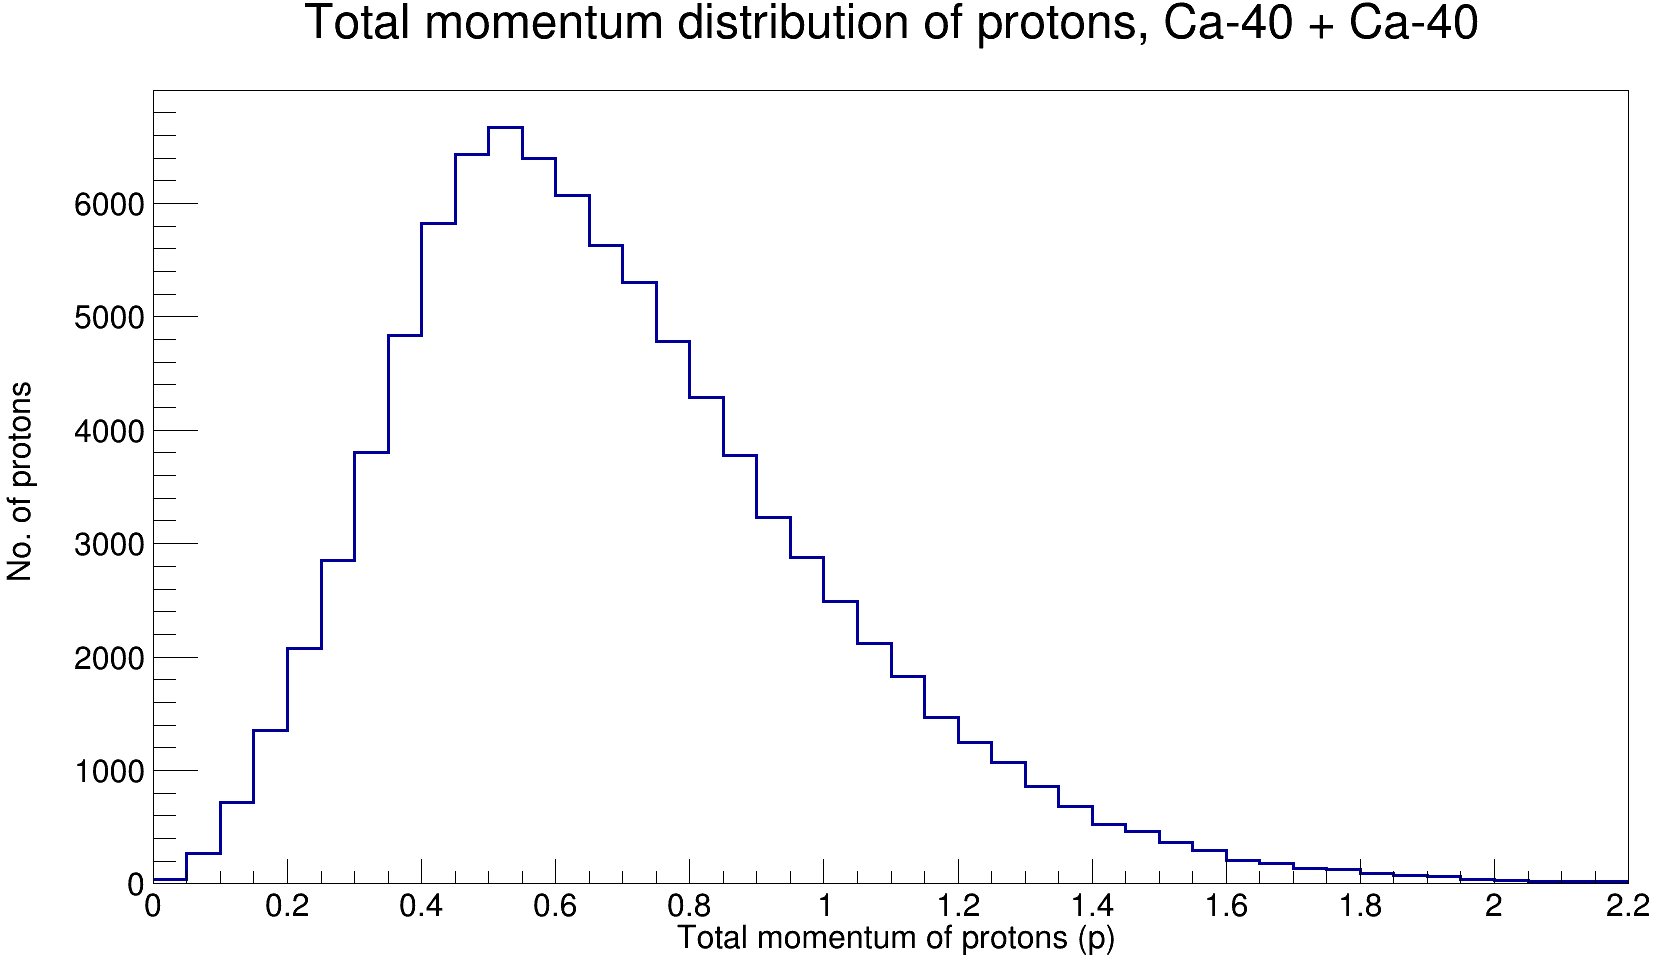
\includegraphics[scale=0.14]{pToT_protons_Ca.png}
\caption{p distribution of $p^{\pm}$ in $^{40}Ca-{^{40}Ca}$ collision.}
\label{Generator - Total momentum distribution of protons Ca40.}
\end{subfigure}
\hfill
\begin{subfigure}[h]{0.49\textwidth}
\centering
\includegraphics[scale=0.14]{pToT_Pions_C12.png}
\caption{p distribution of $\pi^{\pm}$ in $^{12}C-{^{12}C}$ collision.}
\label{Generator - Total momentum distribution of pions C12.}
\end{subfigure}
\hfill
\vspace*{1cm}
\begin{subfigure}[h]{0.49\textwidth}
\centering
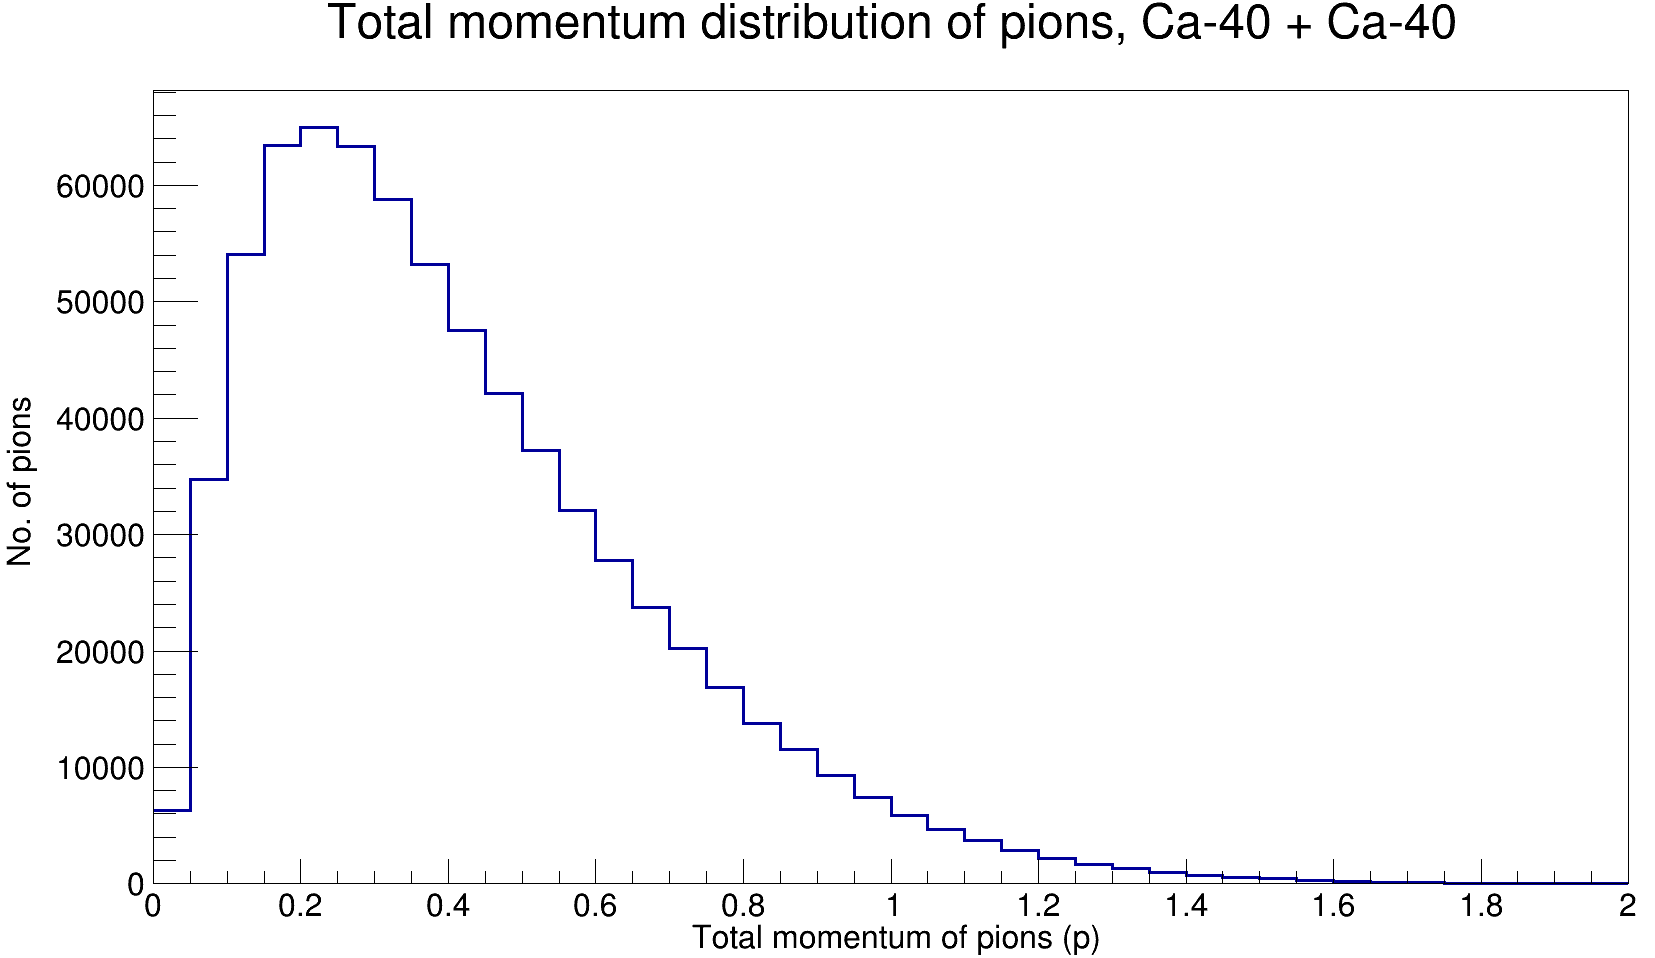
\includegraphics[scale=0.14]{pToT_pions_Ca.png}
\caption{p distribution of $\pi^{\pm}$ in $^{40}Ca-{^{40}Ca}$ collision.}
\label{Generator - Total momentum distribution of pions Ca40.}
\end{subfigure}
\hfill
\begin{subfigure}[h]{0.49\textwidth}
\centering
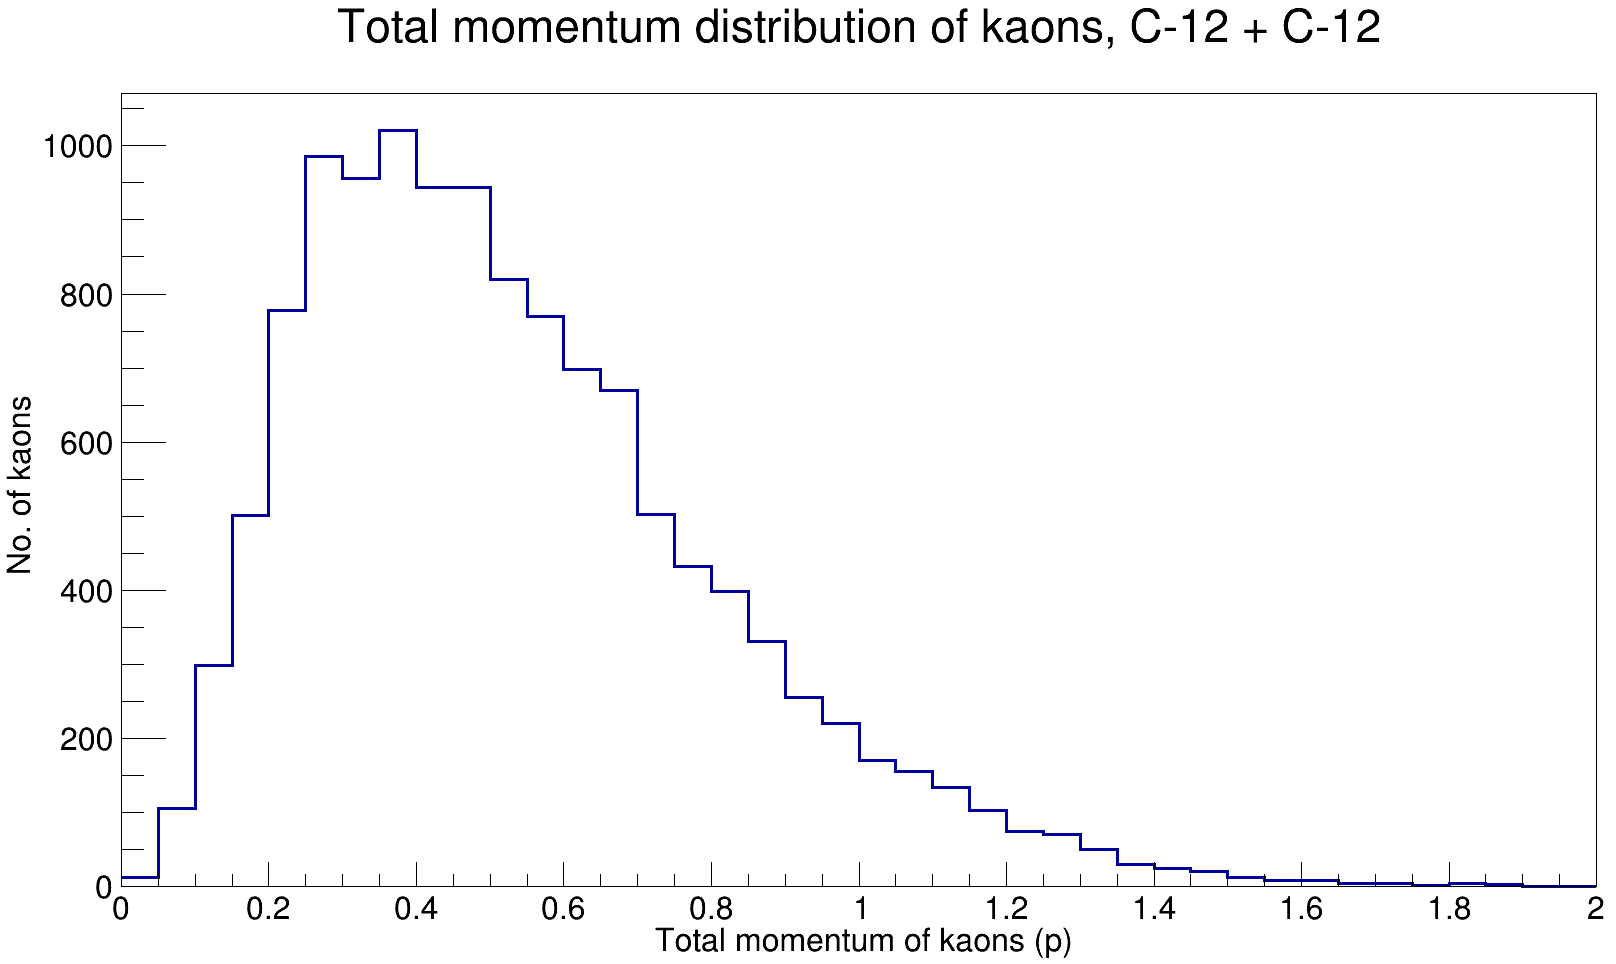
\includegraphics[scale=0.14]{pToT_kaons_C12.png}
\caption{p distribution of $k^{\pm}$ in $^{12}C-{^{12}C}$ collision.}
\label{Generator - Total momentum distribution of kaons C12.}
\end{subfigure}
\hfill
\begin{subfigure}[h]{0.49\textwidth}
\centering
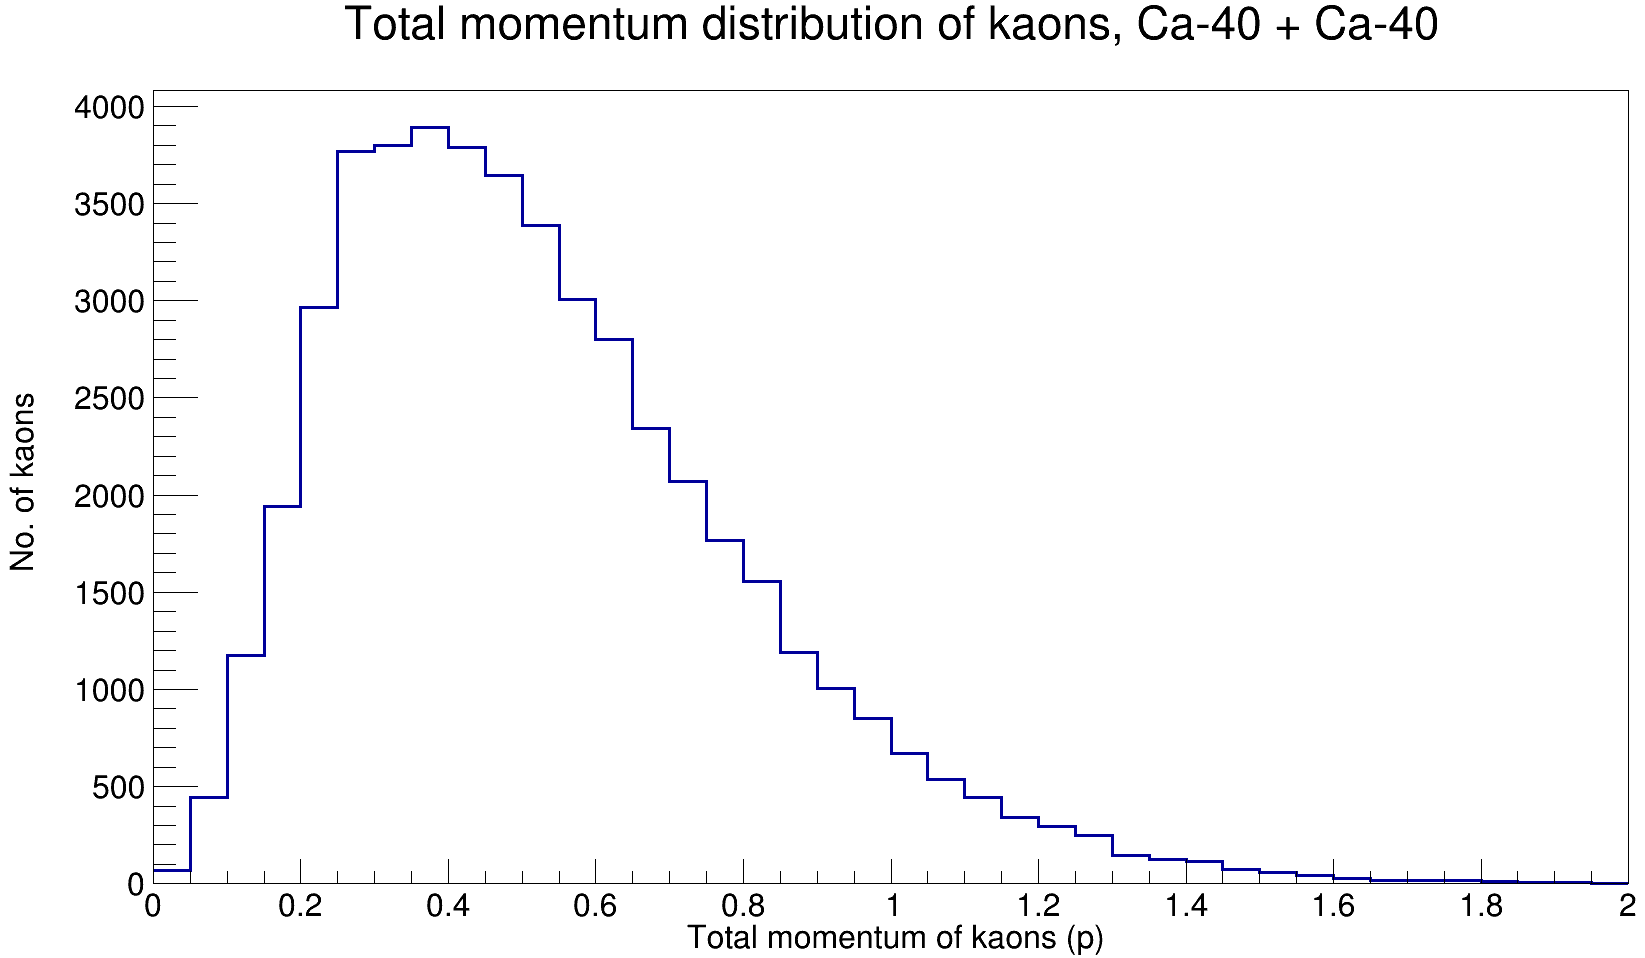
\includegraphics[scale=0.14]{pToT_kaons_Ca.png}
\caption{p distribution of $k^{\pm}$ in $^{40}Ca-{^{40}Ca}$ collision.}
\label{Generator - Total momentum distribution of kaons Ca40.}
\end{subfigure}
\caption{Total momentum distribution of protons, pions, and kaons at generator level in $^{12}C-{^{12}C}$ and $^{40}Ca-{^{40}Ca}$ collision.}
\label{Total momentum distribution of protons, pions, and kaons at generator level in C12-C12 and Ca-Ca40 collision.}
\end{figure*}

\clearpage

\begin{figure*}[h]
\centering
\begin{subfigure}[h]{0.49\textwidth}
\centering
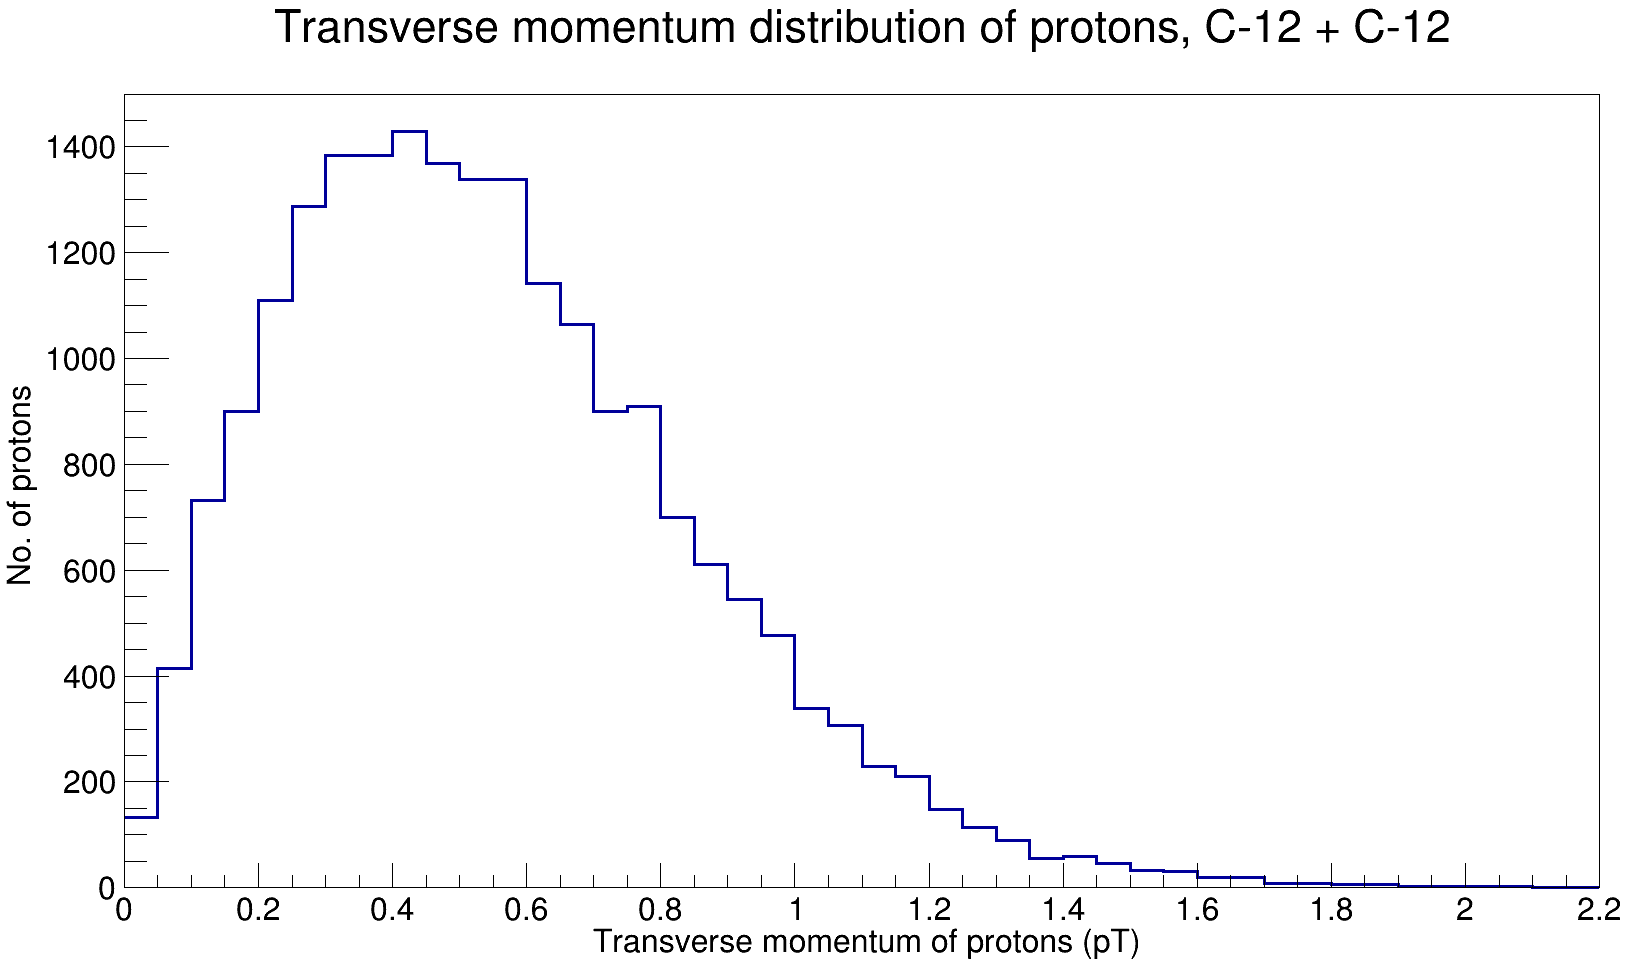
\includegraphics[scale=0.14]{pT_protons_C12.png}
\caption{pT distribution of $p^{\pm}$ in $^{12}C-{^{12}C}$ collision.}
\label{Generator - Transverse momentum distribution of protons C12.}
\end{subfigure}
\hfill
\vspace*{1cm}
\begin{subfigure}[h]{0.49\textwidth}
\centering
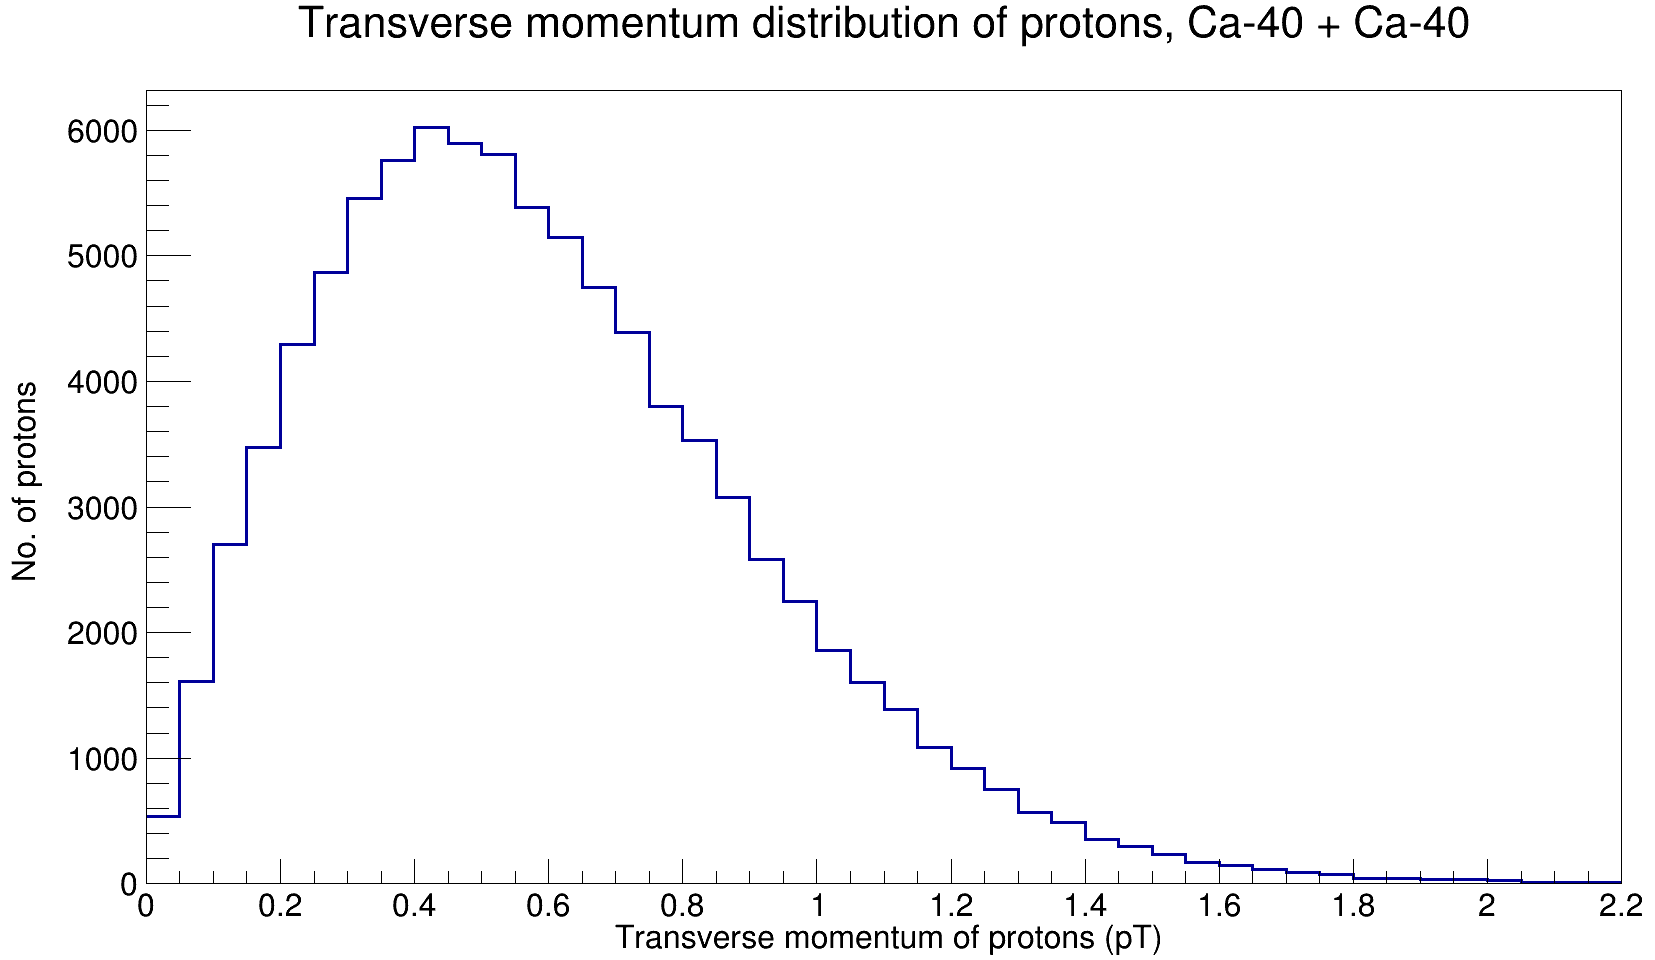
\includegraphics[scale=0.14]{pT_protons_Ca.png}
\caption{pT distribution of $p^{\pm}$ in $^{40}Ca-{^{40}Ca}$ collision.}
\label{Generator - Transverse momentum distribution of protons Ca40.}
\end{subfigure}
\par
\hfill
\begin{subfigure}[h]{0.49\textwidth}
\centering
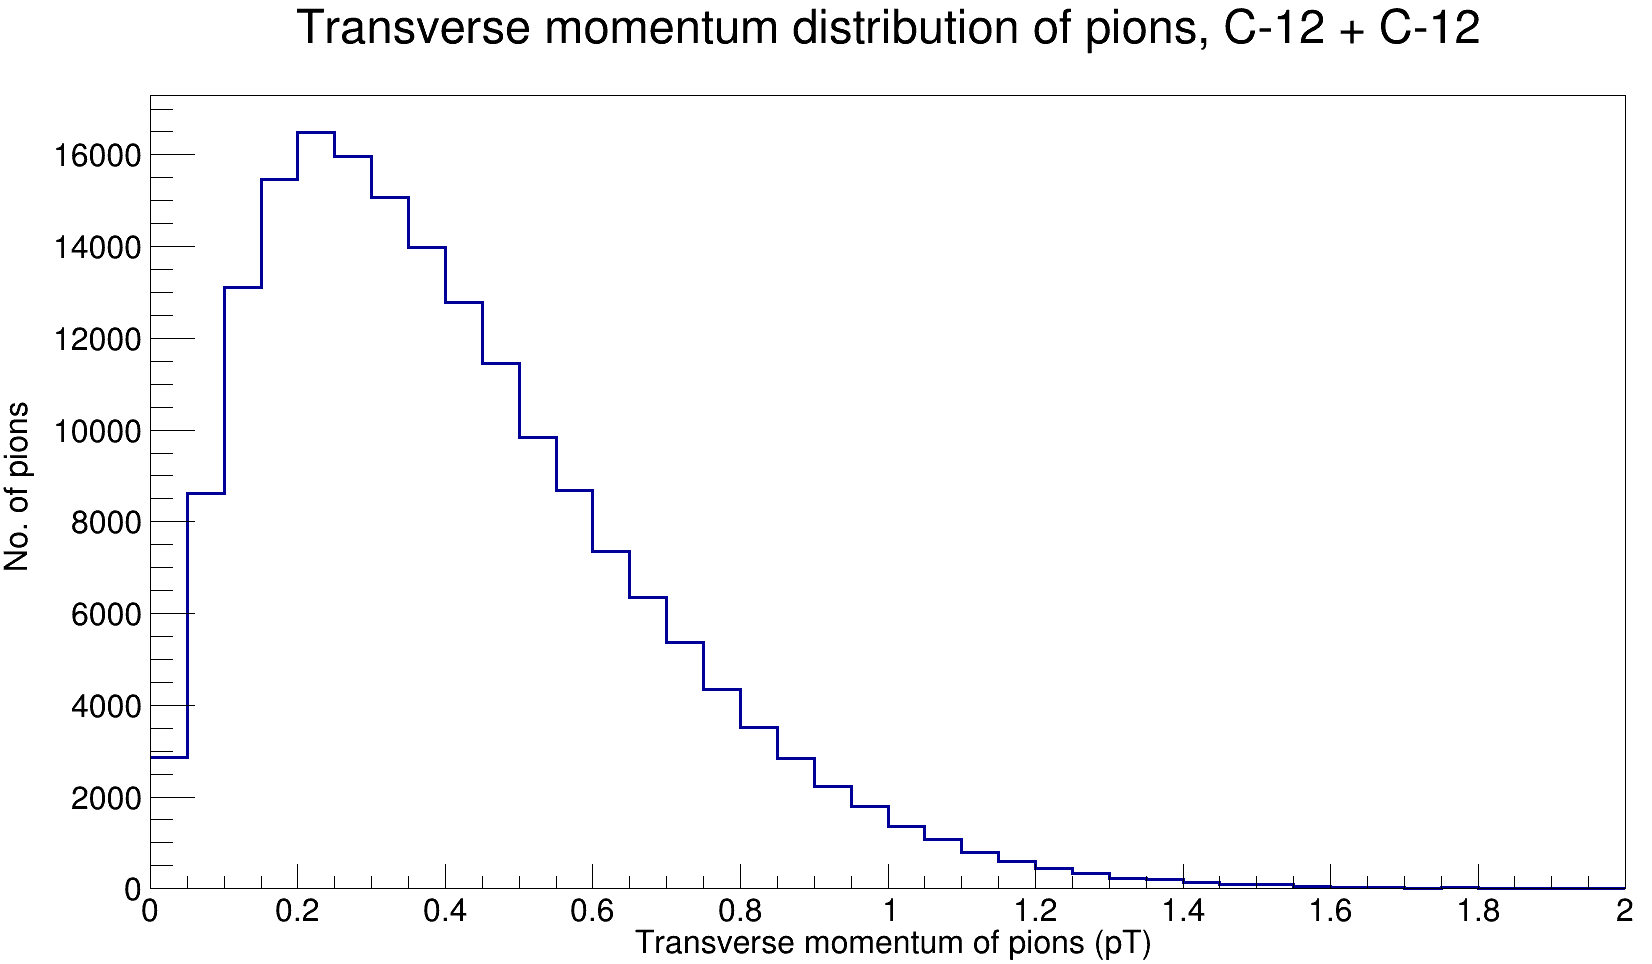
\includegraphics[scale=0.14]{pT_Pions_C12.png}
\caption{pT distribution of $\pi^{\pm}$ in $^{12}C-{^{12}C}$ collision.}
\label{Generator - Transverse momentum distribution of pions C12.}
\end{subfigure}
\hfill
\vspace*{1cm}
\begin{subfigure}[h]{0.49\textwidth}
\centering
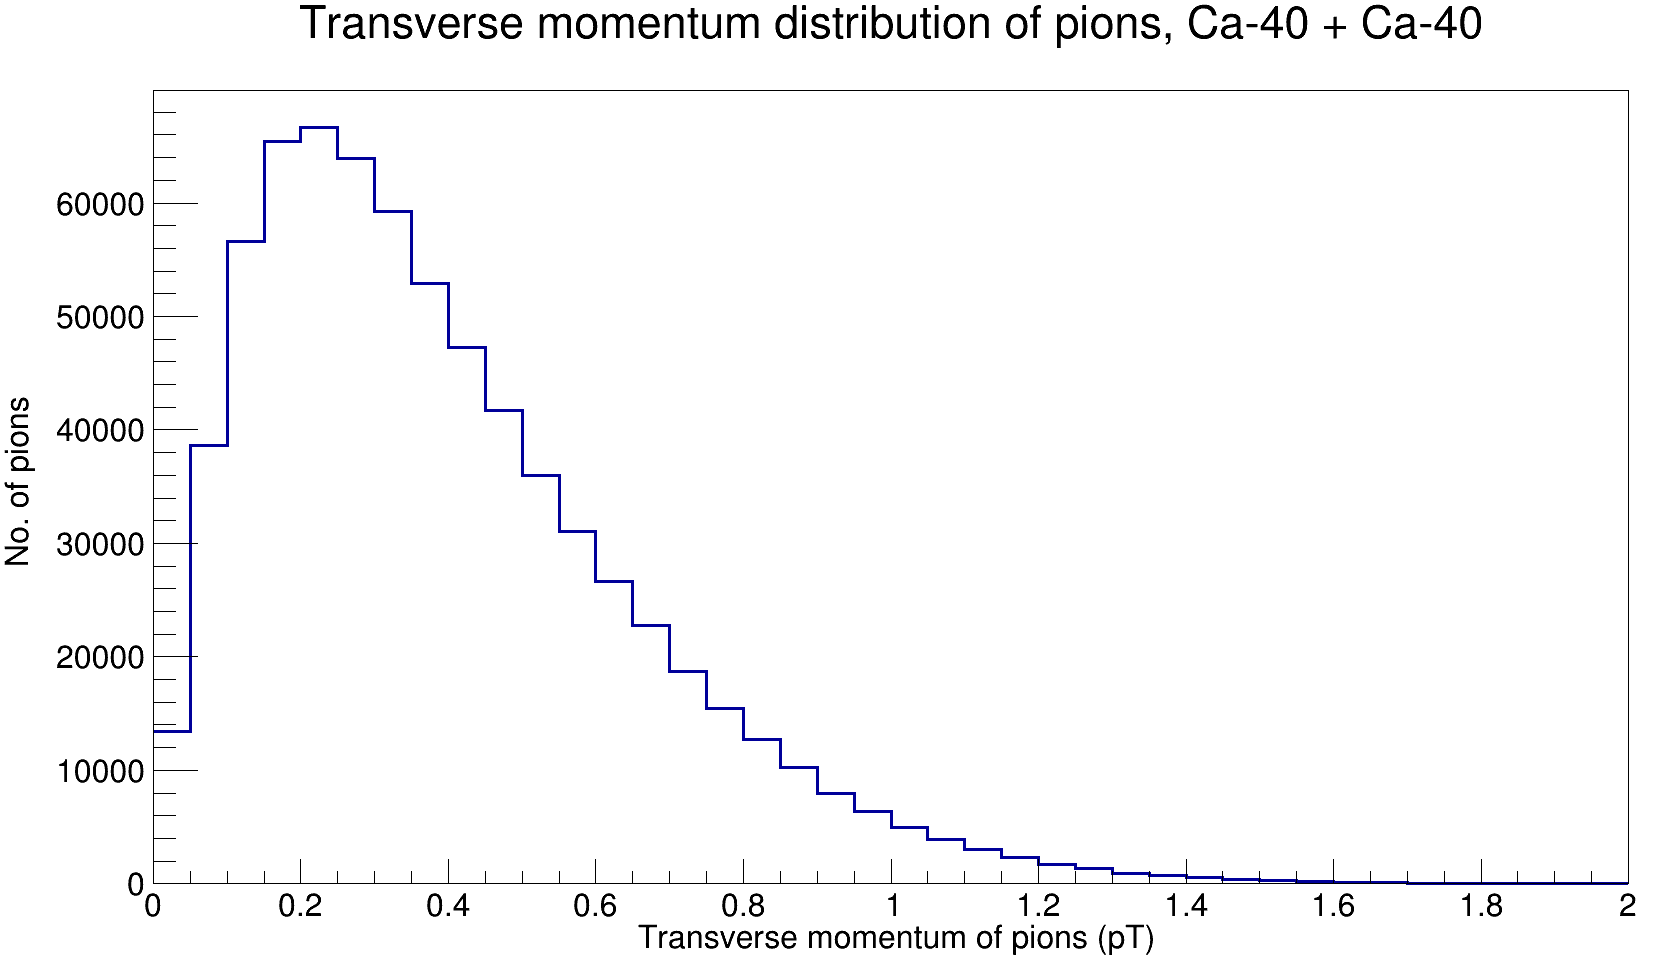
\includegraphics[scale=0.14]{pT_pions_Ca.png}
\caption{pT distribution of $\pi^{\pm}$ in $^{40}Ca-{^{40}Ca}$ collision.}
\label{Generator - Transverse momentum distribution of pions Ca40.}
\end{subfigure}
\par
\hfill
\begin{subfigure}[h]{0.49\textwidth}
\centering
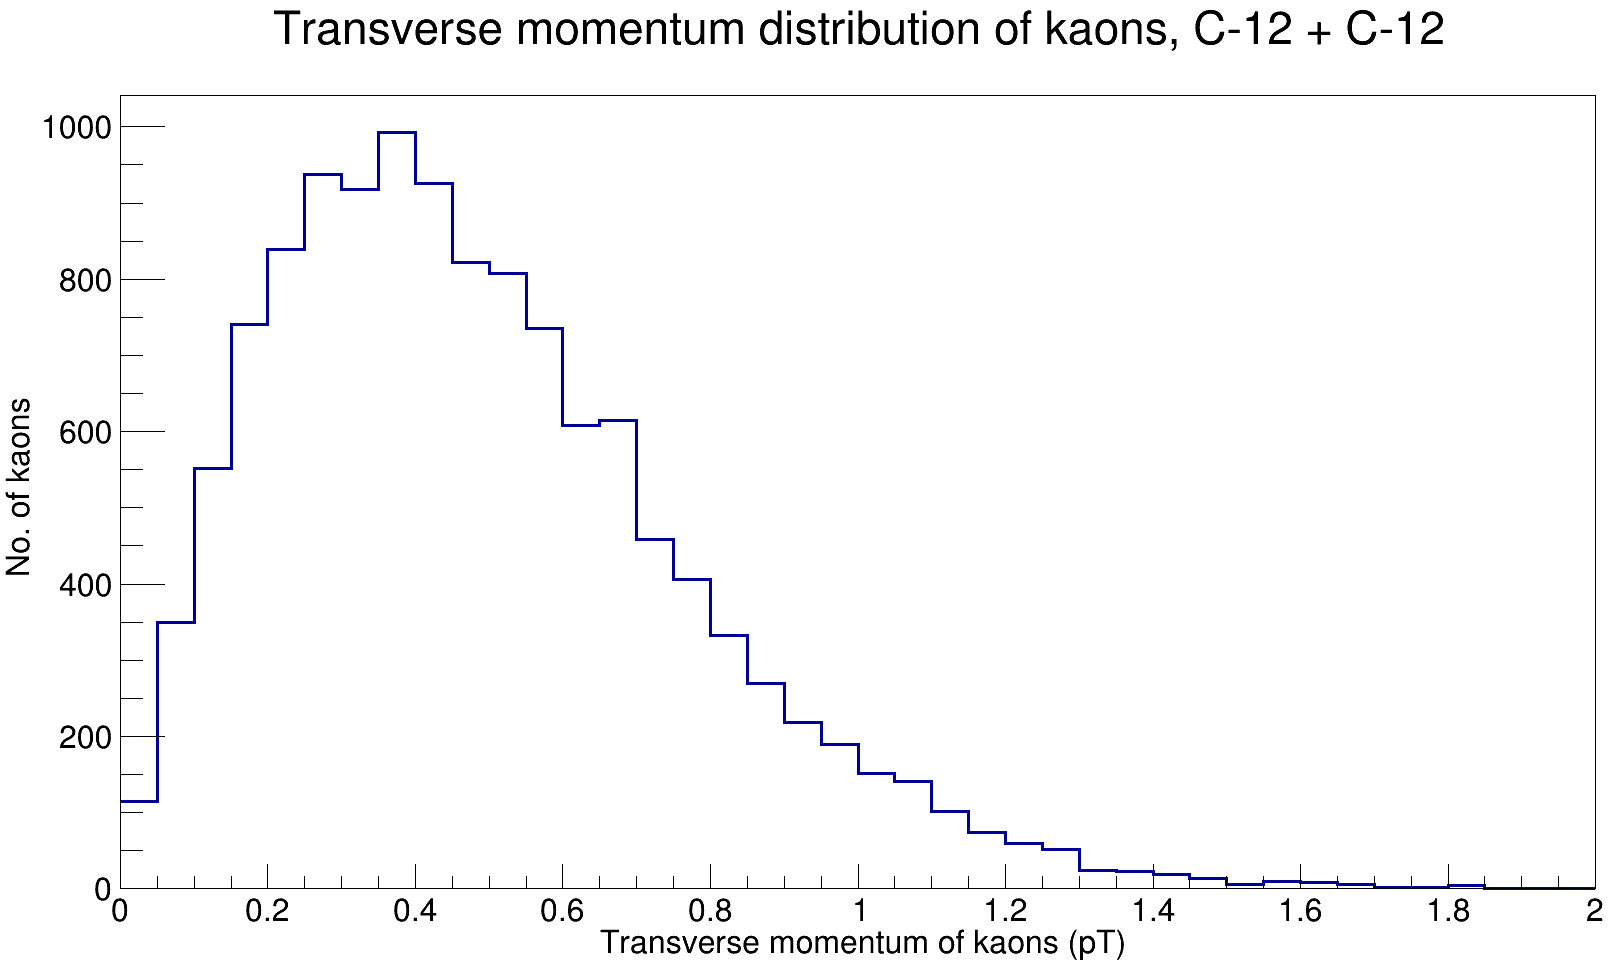
\includegraphics[scale=0.14]{pT_kaons_C12.png}
\caption{pT distribution of $k^{\pm}$ in $^{12}C-{^{12}C}$ collision.}
\label{Generator - Transverse momentum distribution of kaons C12.}
\end{subfigure}
\hfill
\begin{subfigure}[h]{0.49\textwidth}
\centering
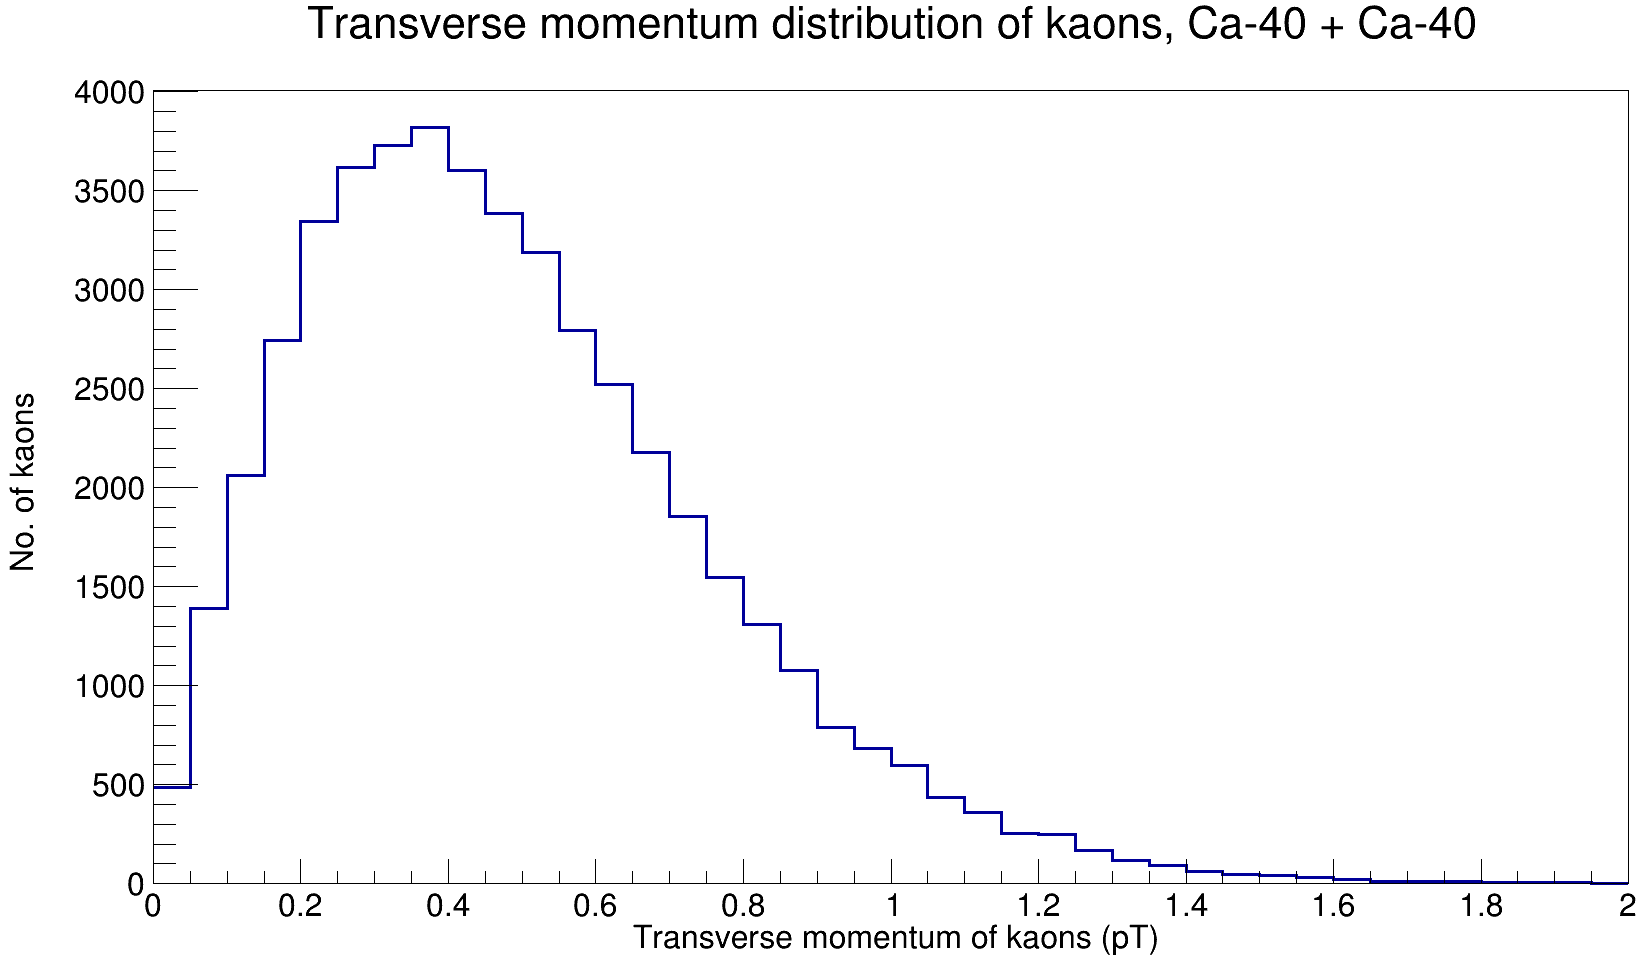
\includegraphics[scale=0.14]{pT_kaons_Ca.png}
\caption{pT distribution of $k^{\pm}$ in $^{40}Ca-{^{40}Ca}$ collision.}
\label{Generator - Transverse momentum distribution of kaons Ca40.}
\end{subfigure}
\caption{Transverse momentum distribution of protons, pions, and kaons at generator level in $^{12}C-{^{12}C}$ and $^{40}Ca-{^{40}Ca}$ collision.}
\label{Transverse momentum distribution of protons, pions, and kaons at generator level in C12-C12 and Ca-Ca40 collision.}
\end{figure*}

\clearpage

\section{DETECTOR SIMULATION AND EVENT RECONSTRUCTION}
The detector simulation and reconstruction is performed with
the SpdRoot framework. To read SMASH generated events the
SpdRoot code has been modified and additional C++ class
was added.
During the simulation stage the particles
were transported through the detector geometrical model using
Geant4. At the reconstruction stage Geant4 tracks and vertices
were reconstructed and particle identification with $dE/dx$ and
time of flight measurements was performed. For the PID three
hypotheses have been considered: pion, kaon and proton.
The reconstructed energy losses and ``measured'' time of flight
were used to construct conditional probabilities (e.g. $P(t|pid)$,
where $t$ is the measured time and $pid$ is a particle type hypothesis).

Out of 100K events generated by SMASH, first 1K events were considered for detector simulation due to slow data processing.

\section{ANALYSIS}
All tracks reconstructed in the detector with measured 
momentum were accepted. For the particle type the one that
gives the largest conditional probability is adopted. Multiplicity, as well as kinematic distributions for
pions, kaons and protons were studied. Analysis of detector level results for both C-C and Ca-Ca heavy ion collisions are described in subsections \ref{DETECTOR LEVEL RESULTS IN C-C HEAVY ION COLLISION}, and \ref{DETECTOR LEVEL RESULTS IN Ca-Ca HEAVY ION COLLISION} respectively.

%%%%%%%%%%%%%%%%%%%%%% Start of C12-C12 analysis %%%%%%%%%%%%%%%%%%%%%%%

\subsection{DETECTOR LEVEL RESULTS IN $^{12}C-{^{12}C}$ HEAVY ION COLLISION}
\label{DETECTOR LEVEL RESULTS IN C-C HEAVY ION COLLISION}
After particle generation, detector simulation, and track reconstruction, a physical analysis was performed using C++ codes and ROOT library. The analysis script was designed in such a way, that it extracted informations like momentum, pdg codes, conditional probabilities, ionization loss - $dE/dx$ (for ST particles), and mass-squared (for TOF particles) of the charged tracks. Further, these informations were used to plot charged track multiplicities, and kinematic distributions of pions, kaons, and protons at detector level. For C-C collision, charged track multiplicity and different charged particle spectra have been discussed below. 

\subsubsection{CHARGED TRACK MULTIPLICITY, $^{12}C-{^{12}C}$}
\label{CHARGED TRACK MULTIPLICITY, C12-C12}
Fig.\ref{Total multiplicity of charged particles passing through tracking system. Red-dashed line is for charged particles passing through ST, and blue line is for charged particles passing through TOF, in C12-C12 collision (Detector stage).} shows the total multiplicity of charged particles passing through the tracking system. On the detector side, it's important to know the average number of charged particles that hit the tracking system per event than simply the average number of charged particles per event. This is because in few events some of the charged tracks escapes the tracking system without identification. The geometry of the tracking system is such that, tracks with polar angle, $\theta < 10^{\circ}$ or $> 170^{\circ}$ do not hit the tracker and passes along the beam pipe itself, so such tracks are ignored. Hence, in the plot of total multiplicity of charged particles passing through tracking system, the X-axis count starts from 1 rather than 0. It was observed that the maximum number of events had only 1 charged track passing through the tracking system. This is due to in most of the events there were few outgoing particles (like 24, $12 p^{+} + 12 n^{0}$) during simulation of C-C collision in SMASH. On performing track reconstruction, there were many events in which 0, 1, 2 tracks were only reconstructed. However, events with no tracks can be ignored, but events with 1 track can't.

\begin{figure}[h]
\centering
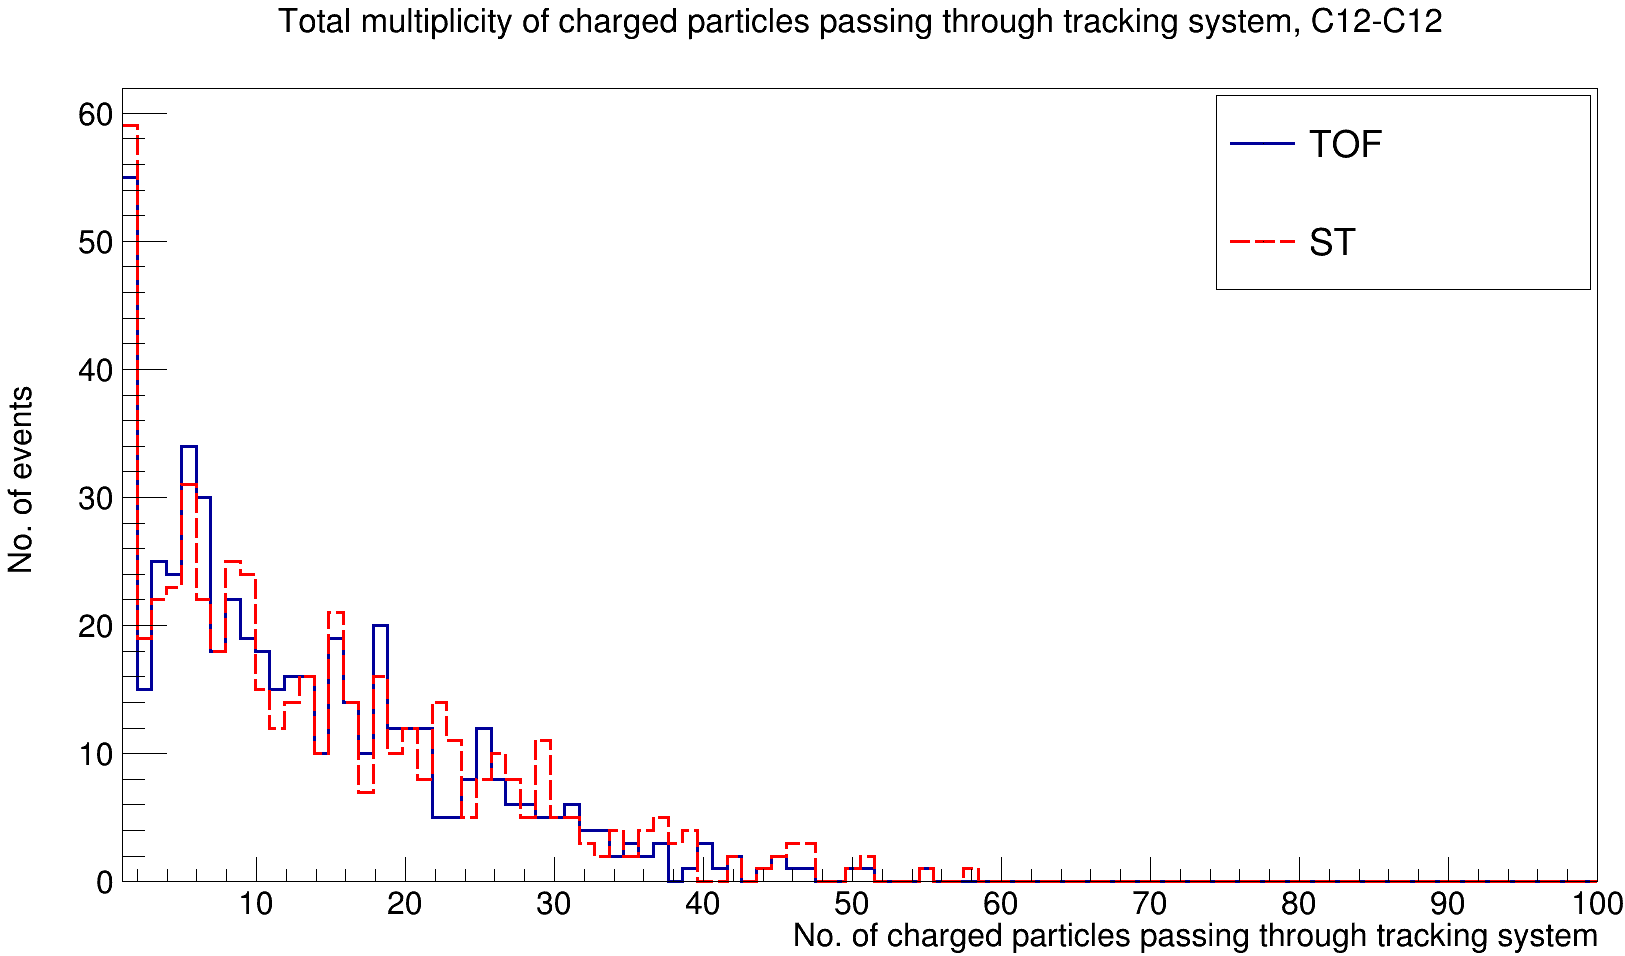
\includegraphics[scale=0.14]{Detector_TotalMultiplicity_C12.png}
\caption{Total multiplicity of charged particles passing through tracking system. Red-dashed line is for charged particles passing through ST, and blue line is for charged particles passing through TOF, in $^{12}C-{^{12}C}$ collision (Detector level).}
\label{Total multiplicity of charged particles passing through tracking system. Red-dashed line is for charged particles passing through ST, and blue line is for charged particles passing through TOF, in C12-C12 collision (Detector stage).}
\end{figure}

\subsubsection{PION MOMENTUM (p $\&$ pT) SPECTRA, $^{12}C-{^{12}C}$}
The detector level results of p \& pT - spectra of charged pions are shown by Fig.\ref{Total momentum distribution of charged particles identified as pions in C12-C12 collision.}, and \ref{Transverse momentum distribution of charged particles identified as pions in C12-C12 collision.}. The spectra shows its resemblance with the generator plot of pion momentum distribution. For the individual plots of p \& pT - spectra of charged particles identified as pions by TOF/ST (shown by Fig.\ref{Detector - Total momentum distribution of pions (TOF) C12.}, \ref{Detector - Total momentum distribution of pions (ST) C12.}, \ref{Detector - Transverse momentum distribution of pions (TOF) C12.} \& \ref{Detector - Transverse momentum distribution of pions (ST) C12.}), it has been observed that the dark blue line almost coincides with the brown-dashed one, indicating that `pions identified as pions' is almost same as `different charged particles identified as pions', which further means very few other particles like $k^{\pm}, p^{\pm}, e^{\pm},$ \& $\mu^{\pm}$ were incorrectly identified as pions by TOF/ST during heavy ion collision. Hence, the performance of tracking system for pion identification in heavy ion collision is very good.

\subsubsection{KAON MOMENTUM (p $\&$ pT) SPECTRA, $^{12}C-{^{12}C}$}
\label{KAON MOMENTUM (p and pT) SPECTRA, C12-C12}
Fig.\ref{Total momentum distribution of charged particles identified as kaons in C12-C12 collision.}, and \ref{Transverse momentum distribution of charged particles identified as kaons in C12-C12 collision.} shows the p \& pT spectra of charged particles identified as kaons by tracking system in C-C collision. It has been observed that some electrons and muons were also identified as kaons although they were not generated during the collision. This is because some uncharged primary particles (like high energetic photons) travels some distance undetected before they decay into some stable charged particles which are latter on detected by tracking system. This is one of the way in which leptons are reconstructed (even so not generated) during this process at SPD. Mutual interactions among particles could be the other reason also. The performance of tracking system in kaon identification during heavy ion collision doesn't seems to be good. There are more other particles that are incorrectly identified as kaons than true kaons itself. For eg. in Fig.\ref{Detector - Total momentum distribution of kaons (ST) C12.}, and \ref{Detector - Transverse momentum distribution of kaons (ST) C12.}, for $p > 0.6$ \& $pT > 0$ more pions (shown by red-dashed) were incorrectly identified as kaons than actual kaons itself.

\subsubsection{PROTON MOMENTUM (p $\&$ pT) SPECTRA, $^{12}C-{^{12}C}$}
\label{PROTON MOMENTUM (p and pT) SPECTRA, C12-C12}
The detector level results of proton momentum spectra are shown by Fig.\ref{Total momentum distribution of charged particles identified as protons in C12-C12 collision.}, and \ref{Transverse momentum distribution of charged particles identified as protons in C12-C12 collision.}. In this case, the performance of the TOF was comparatively good than ST. It was observed that in TOF system (see Fig.\ref{Detector - Total momentum distribution of protons (TOF) C12.}, \ref{Detector - Transverse momentum distribution of protons (TOF) C12.}), for $p < 0.25$ or $pT < 0.1$ contamination was very high as more pions were incorrectly identified as protons than the true protons itself. For $p > 0.25$ in TOF, the performance was high and precision was good. However, the ST showed less performance than TOF and seems not to be fit for proton identification during heavy ion collision. Hence, in this case we conclude that proton identification in heavy ion collision can be made using TOF but only for $p > 0.25 GeV/c$.

 
%%%%%%%%%%%%%%%%% Momentum (p & pT) Distribution C12-C12  %%%%%%%%%%%%%%

\begin{figure*}[h]
\centering
\begin{subfigure}[h]{0.49\textwidth}
\centering
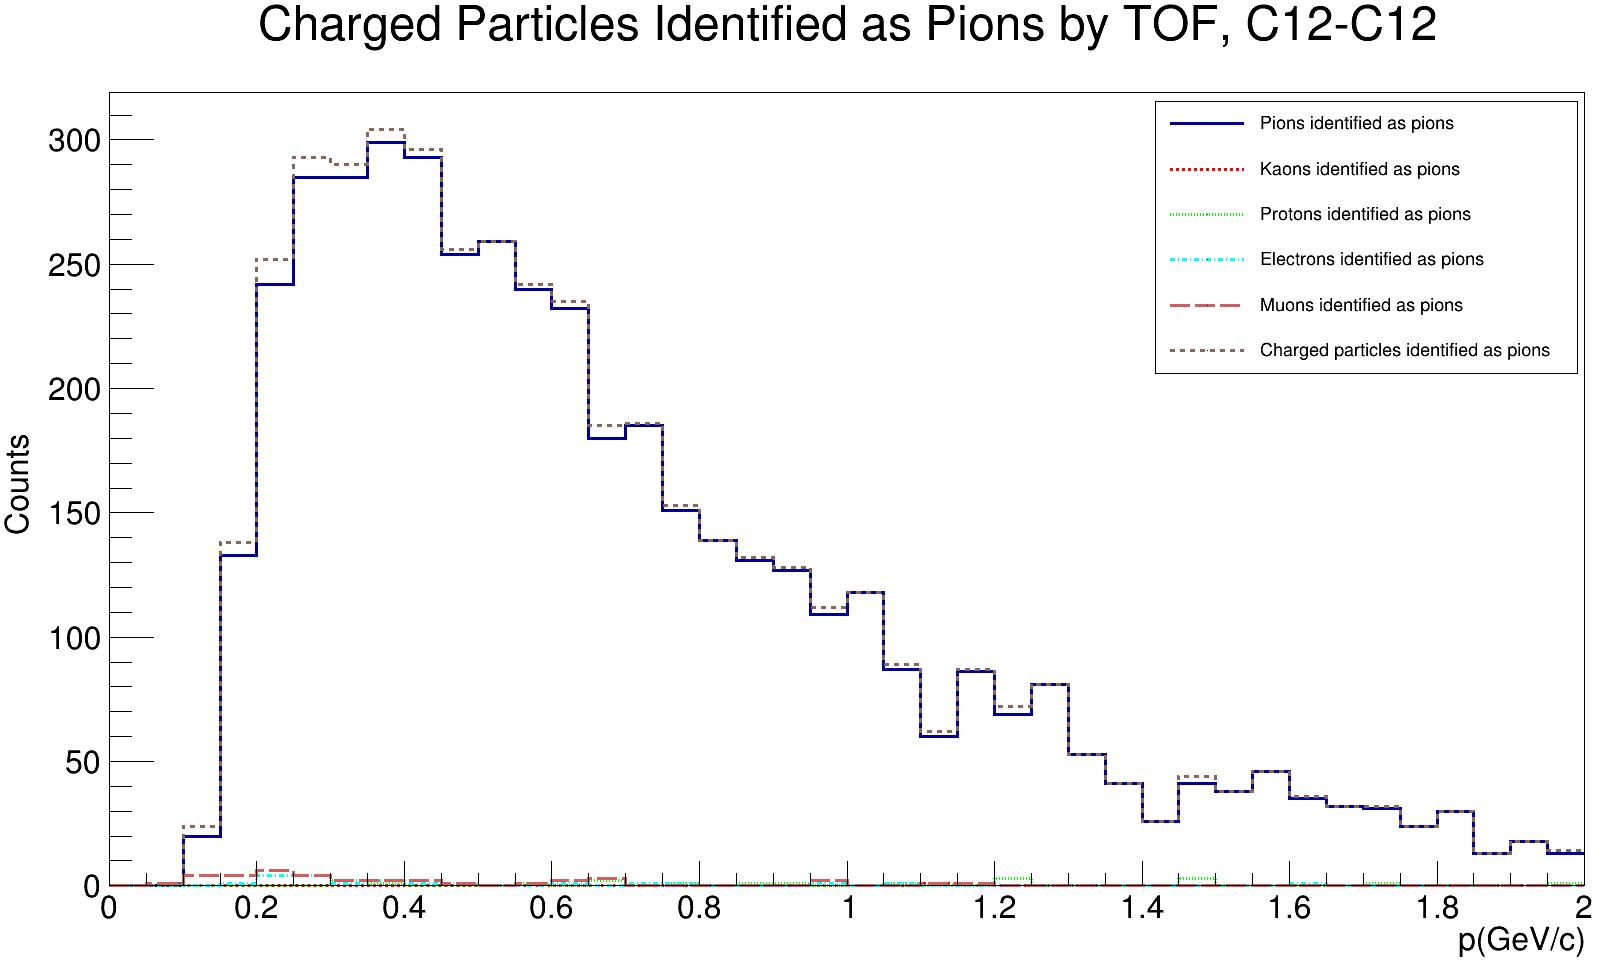
\includegraphics[scale=0.14]{Detector_pToT_pions(tof)_C12.png}
\caption{Total momentum distribution of charged particles identified as $\pi^{\pm}$ by TOF.}
\label{Detector - Total momentum distribution of pions (TOF) C12.}
\end{subfigure}
\hfill
\begin{subfigure}[h]{0.49\textwidth}
\centering
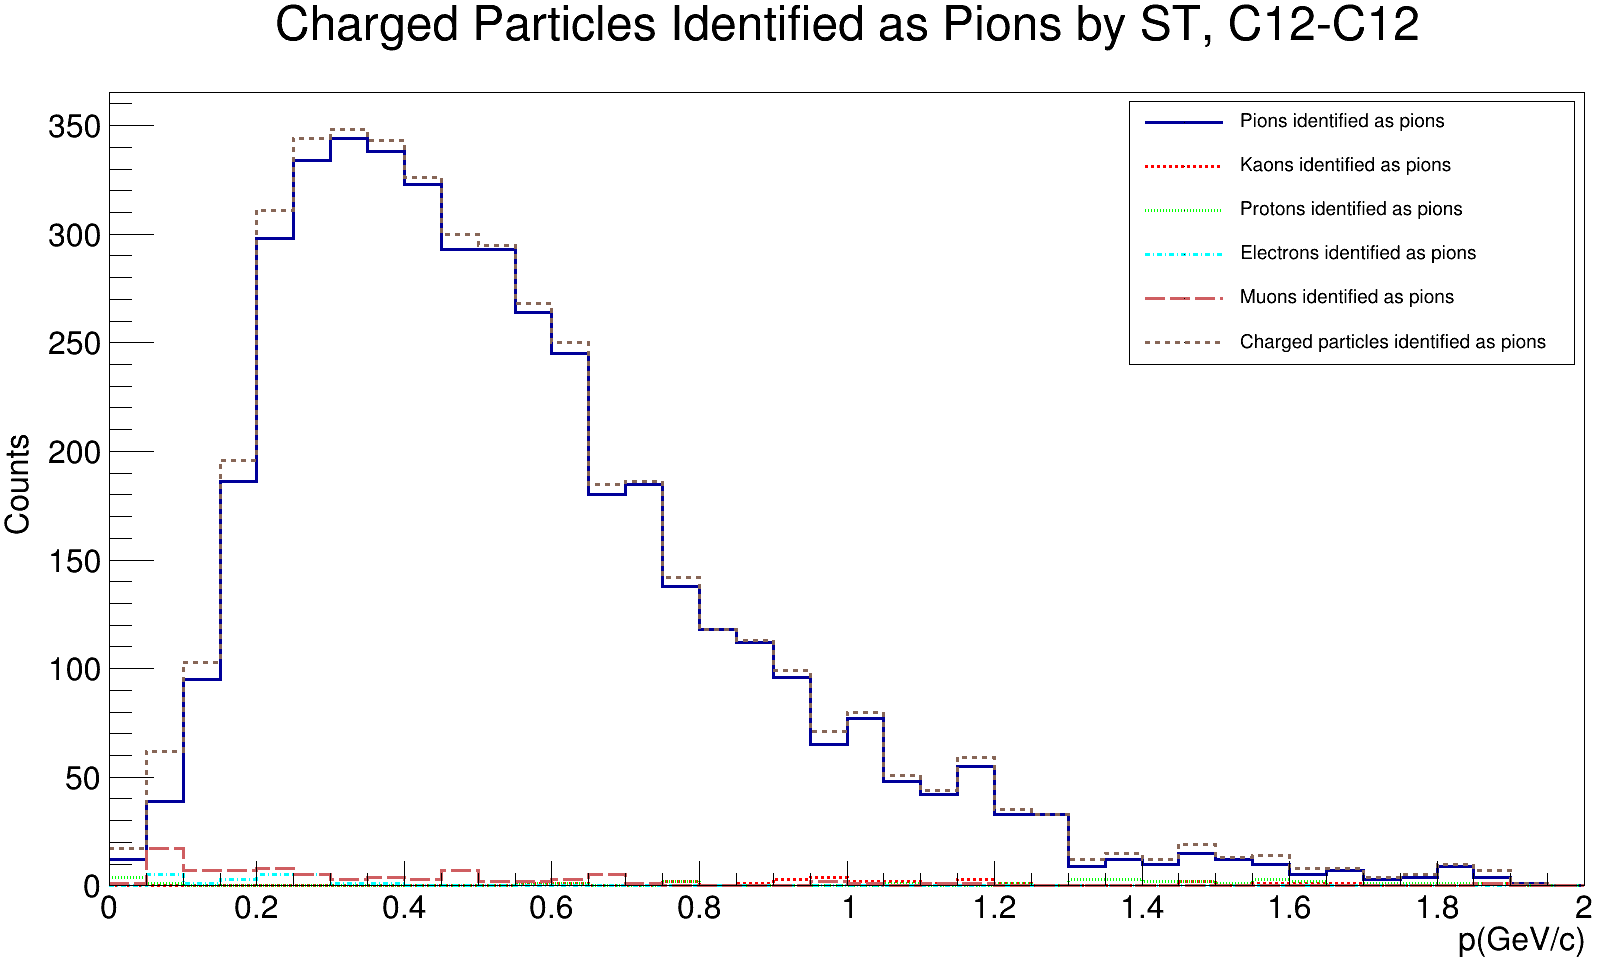
\includegraphics[scale=0.14]{Detector_pToT_pions(st)_C12.png}
\caption{Total momentum distribution of charged particles identified as $\pi^{\pm}$ by ST.}
\label{Detector - Total momentum distribution of pions (ST) C12.}
\end{subfigure}
\caption{Total momentum distribution of charged particles identified as $\pi^{\pm}$ in $^{12}C-{^{12}C}$ collision (Detector level).}
\label{Total momentum distribution of charged particles identified as pions in C12-C12 collision.}
\end{figure*}

\begin{figure*}[h]
\centering
\begin{subfigure}[h]{0.49\textwidth}
\centering
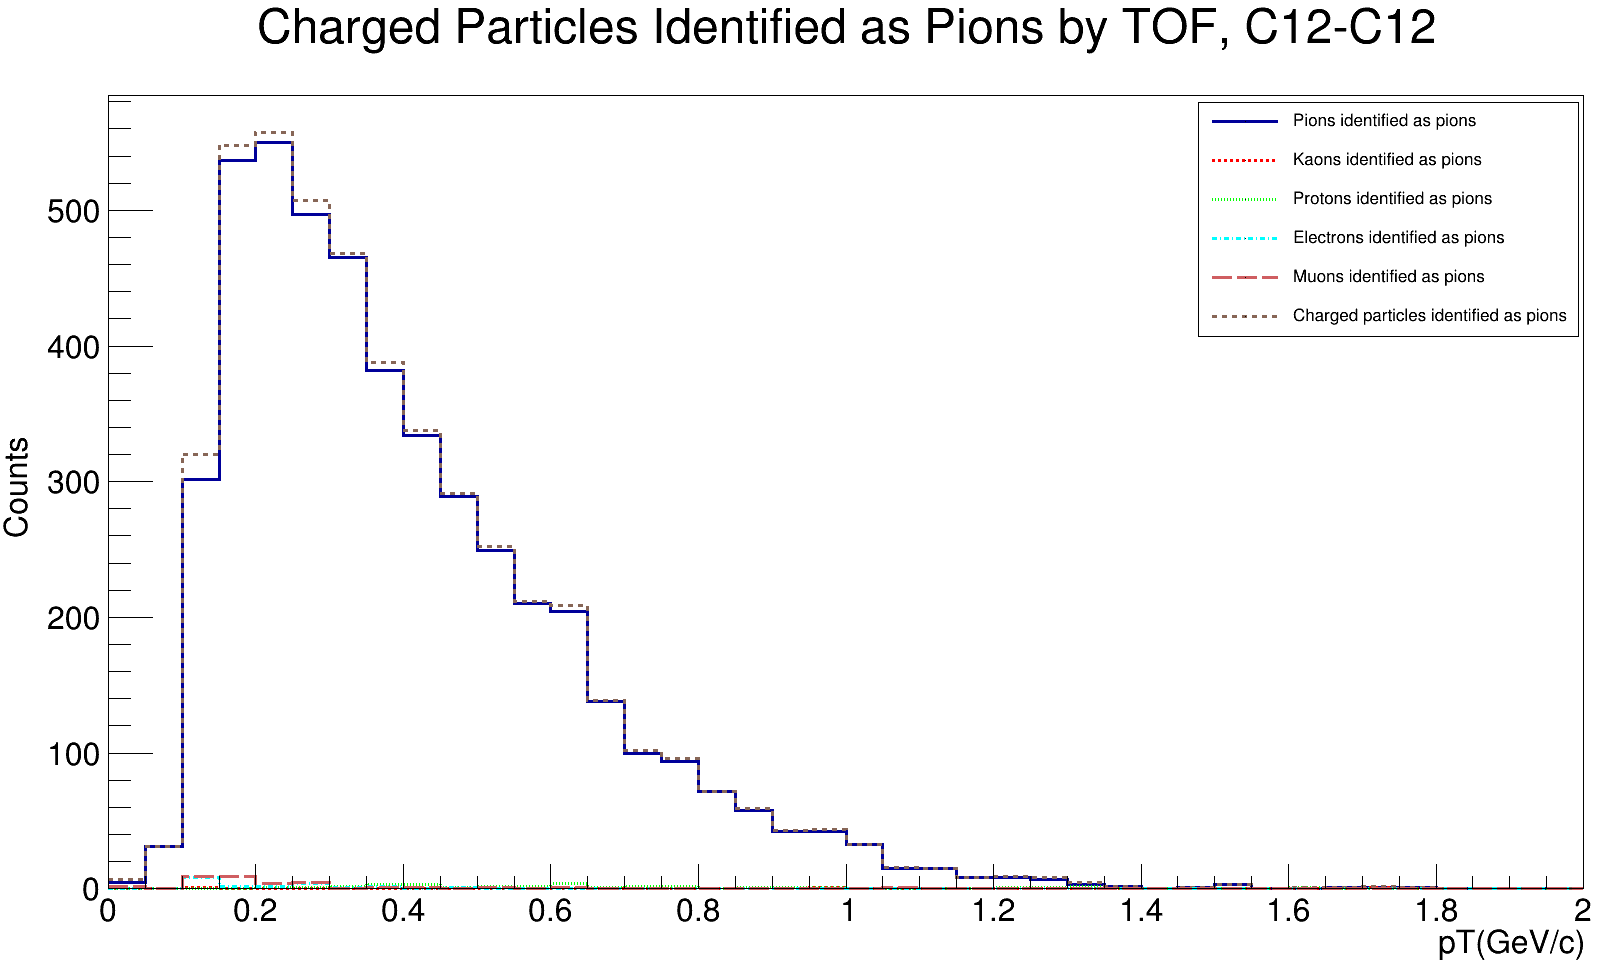
\includegraphics[scale=0.14]{Detector_pT_pions(tof)_C12.png}
\caption{Transverse momentum distribution of charged particles identified as $\pi^{\pm}$ by TOF.}
\label{Detector - Transverse momentum distribution of pions (TOF) C12.}
\end{subfigure}
\hfill
\begin{subfigure}[h]{0.49\textwidth}
\centering
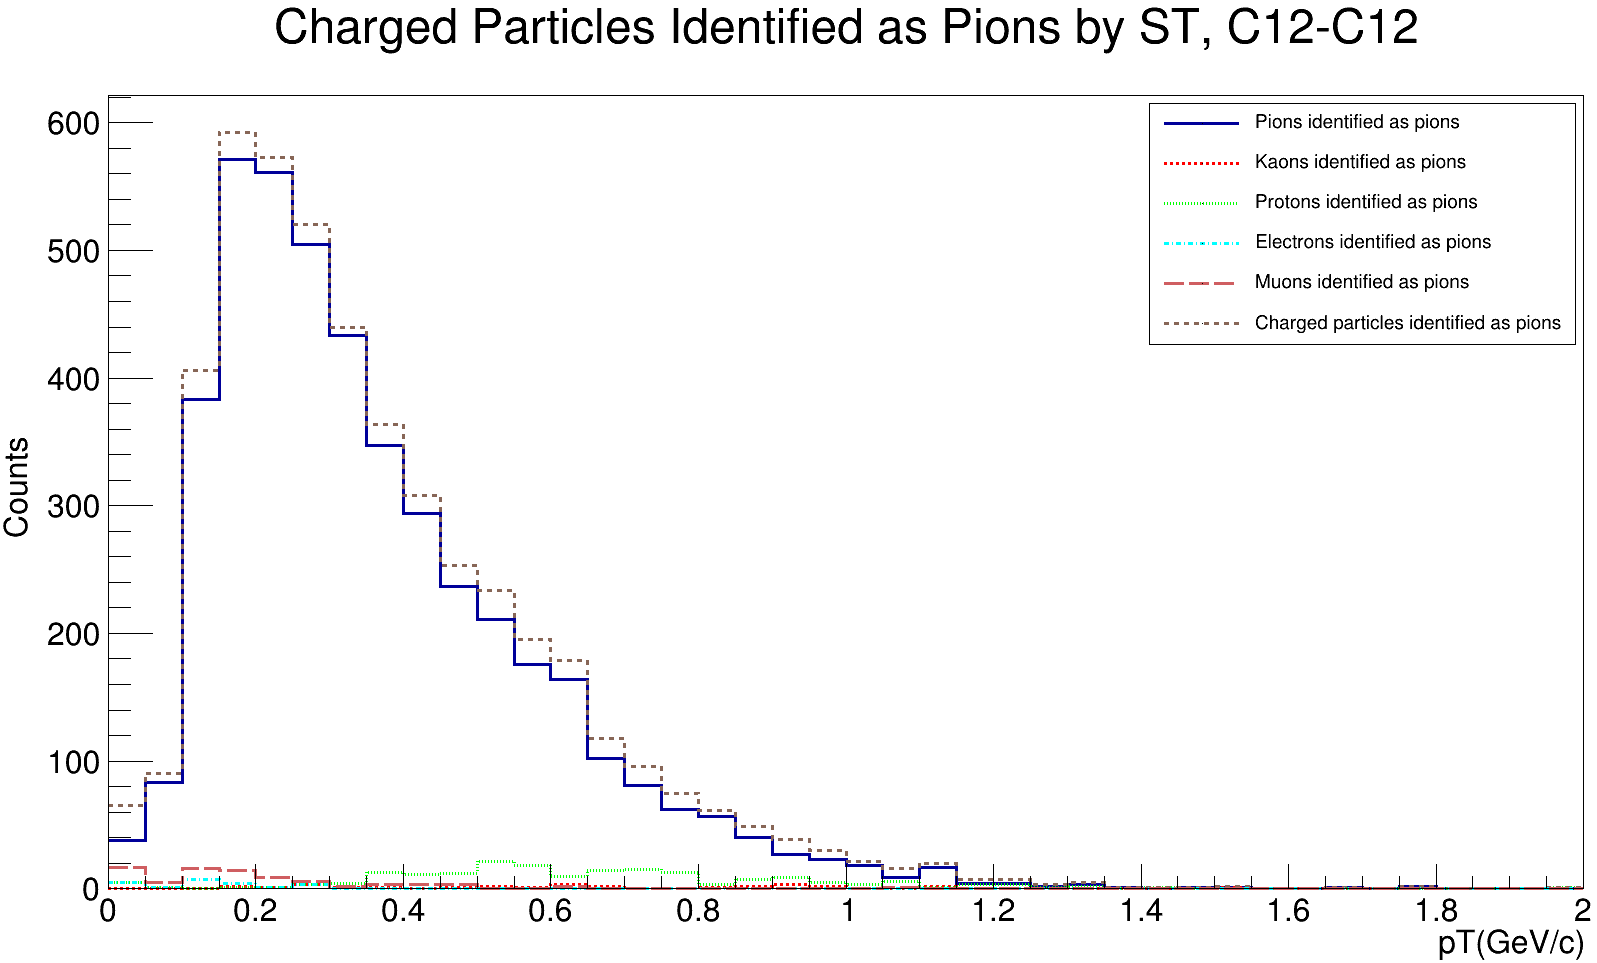
\includegraphics[scale=0.14]{Detector_pT_pions(st)_C12.png}
\caption{Transverse momentum distribution of charged particles identified as $\pi^{\pm}$ by ST.}
\label{Detector - Transverse momentum distribution of pions (ST) C12.}
\end{subfigure}
\caption{Transverse momentum distribution of charged particles identified as $\pi^{\pm}$ in $^{12}C-{^{12}C}$ collision (Detector level).}
\label{Transverse momentum distribution of charged particles identified as pions in C12-C12 collision.}
\end{figure*}

\begin{figure*}[h]
\centering
\begin{subfigure}[h]{0.49\textwidth}
\centering
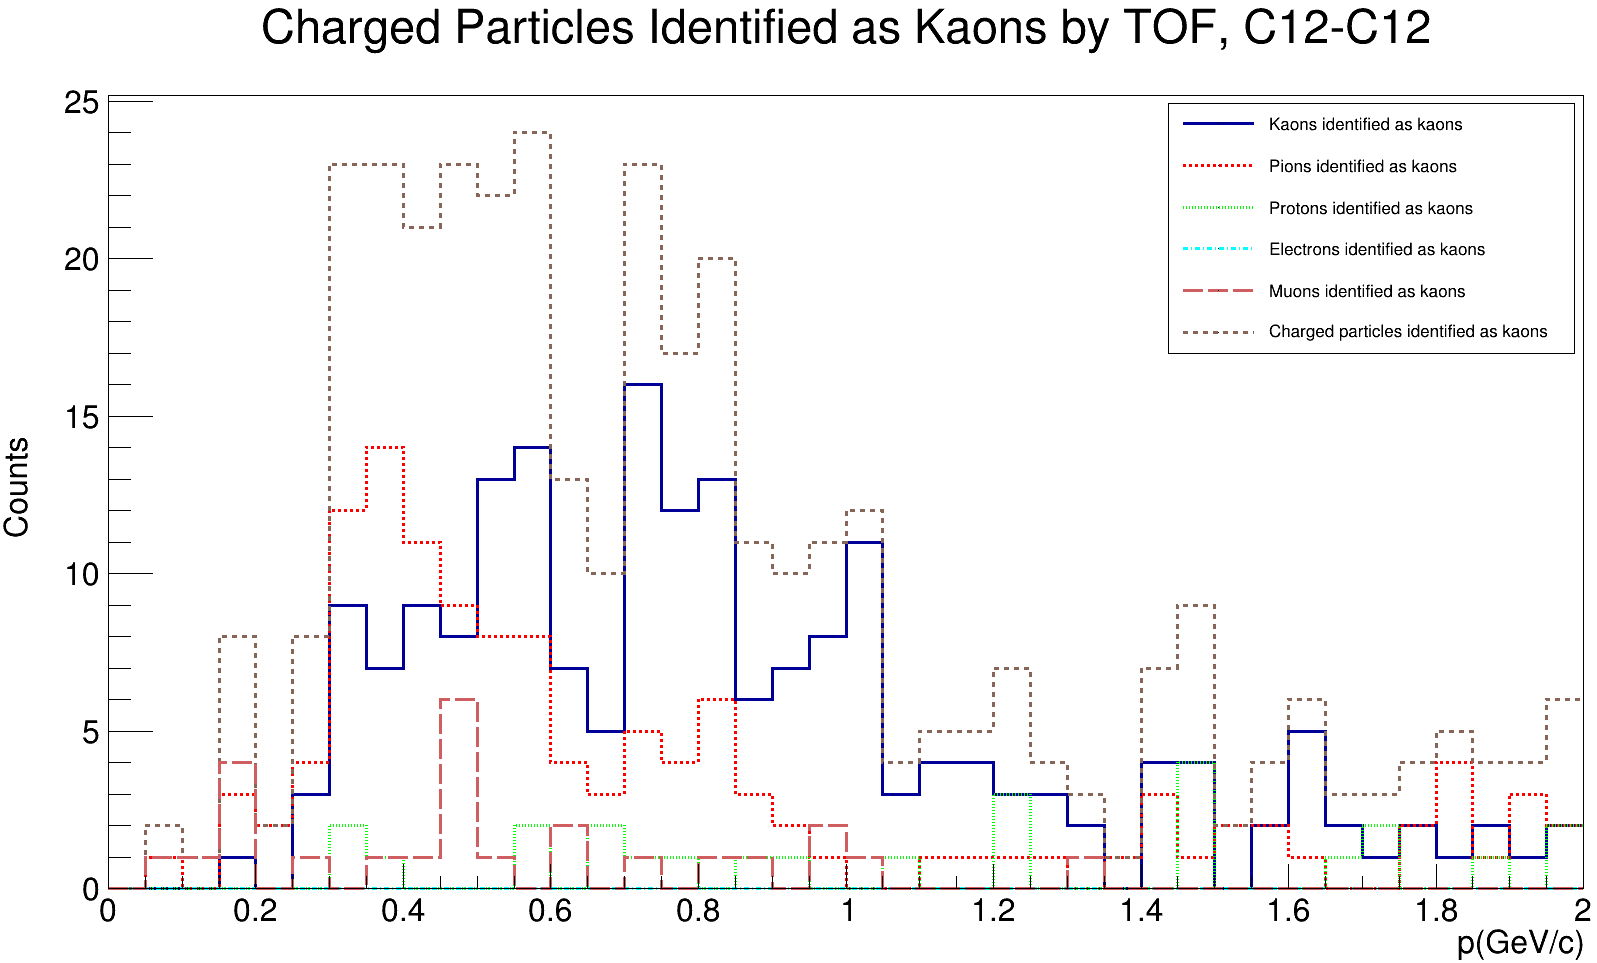
\includegraphics[scale=0.14]{Detector_pToT_kaons(tof)_C12.png}
\caption{Total momentum distribution of charged particles identified as $k^{\pm}$ by TOF.}
\label{Detector - Total momentum distribution of kaons (TOF) C12.}
\end{subfigure}
\hfill
\begin{subfigure}[h]{0.49\textwidth}
\centering
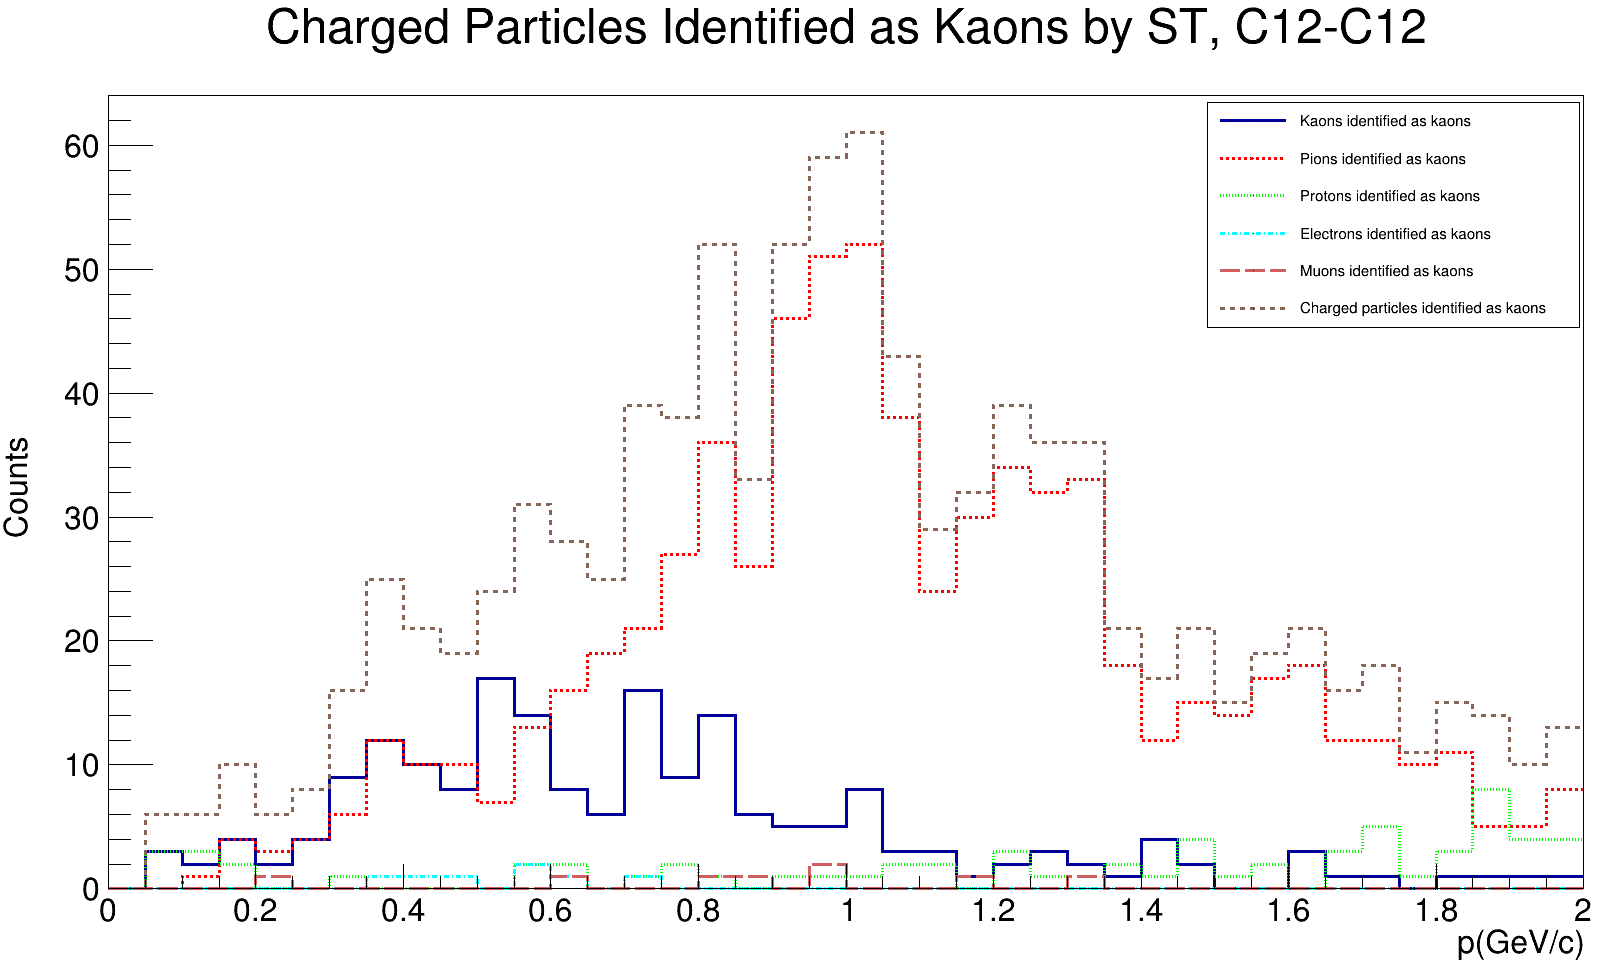
\includegraphics[scale=0.14]{Detector_pToT_kaons(st)_C12.png}
\caption{Total momentum distribution of charged particles identified as $k^{\pm}$ by ST.}
\label{Detector - Total momentum distribution of kaons (ST) C12.}
\end{subfigure}
\caption{Total momentum distribution of charged particles identified as $k^{\pm}$ in $^{12}C-{^{12}C}$ collision (Detector level).}
\label{Total momentum distribution of charged particles identified as kaons in C12-C12 collision.}
\end{figure*}

\clearpage

\begin{figure*}[h]
\centering
\begin{subfigure}[h]{0.49\textwidth}
\centering
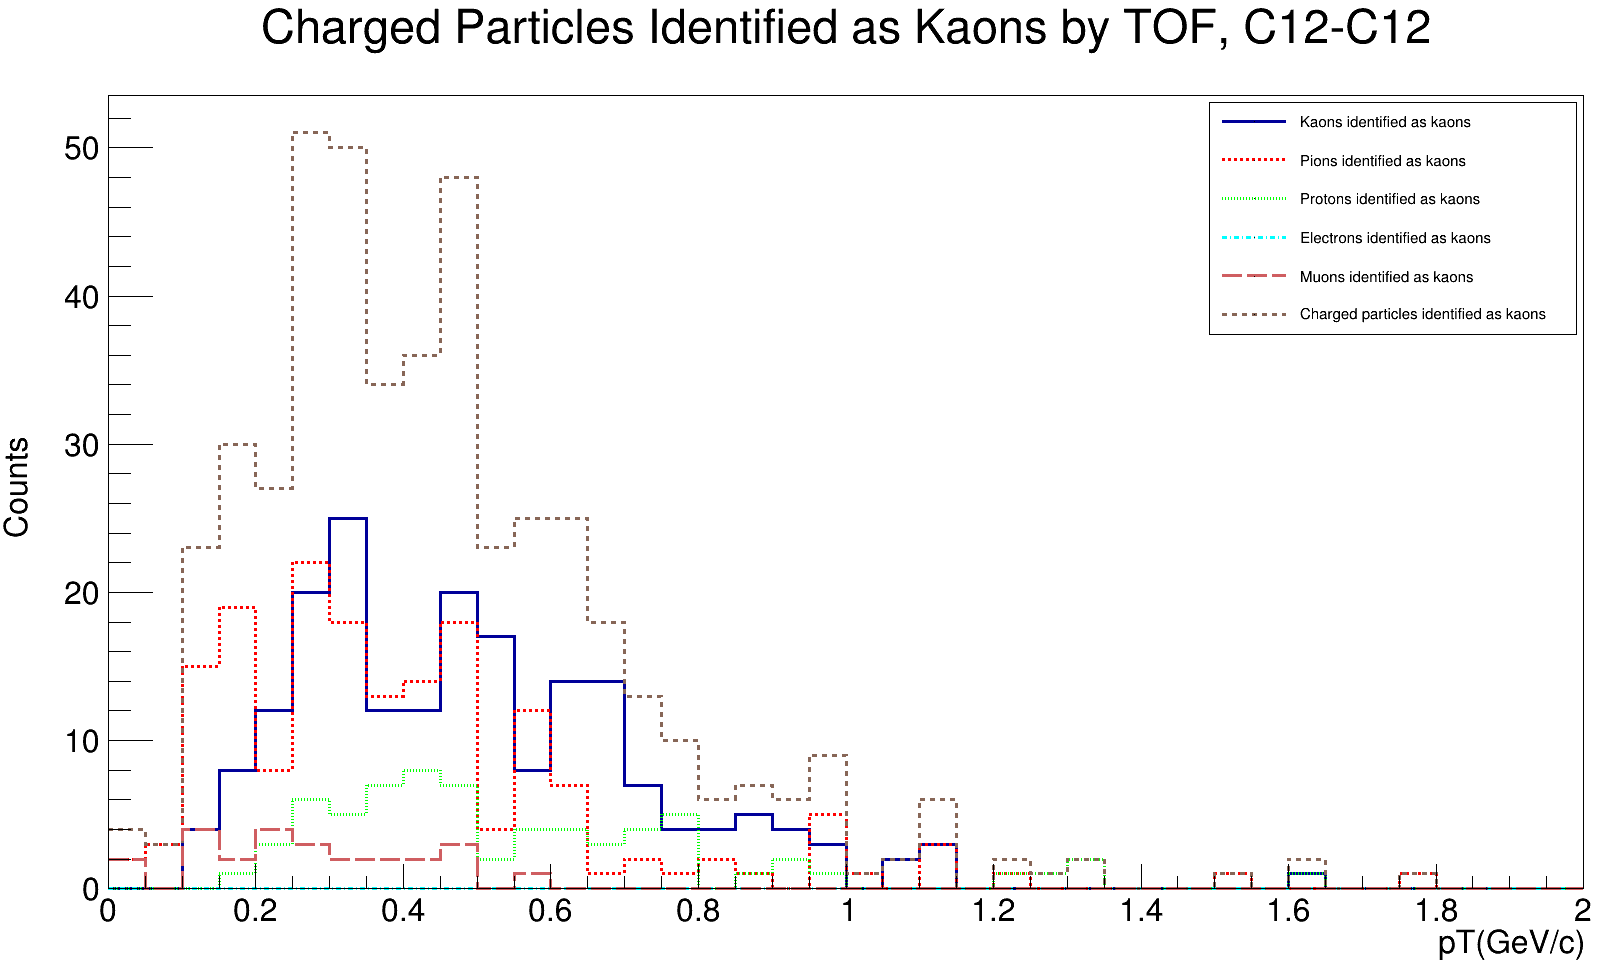
\includegraphics[scale=0.14]{Detector_pT_kaons(tof)_C12.png}
\caption{Transverse momentum distribution of charged particles identified as $k^{\pm}$ by TOF.}
\label{Detector - Transverse momentum distribution of kaons (TOF) C12.}
\end{subfigure}
\hfill
\begin{subfigure}[h]{0.49\textwidth}
\centering
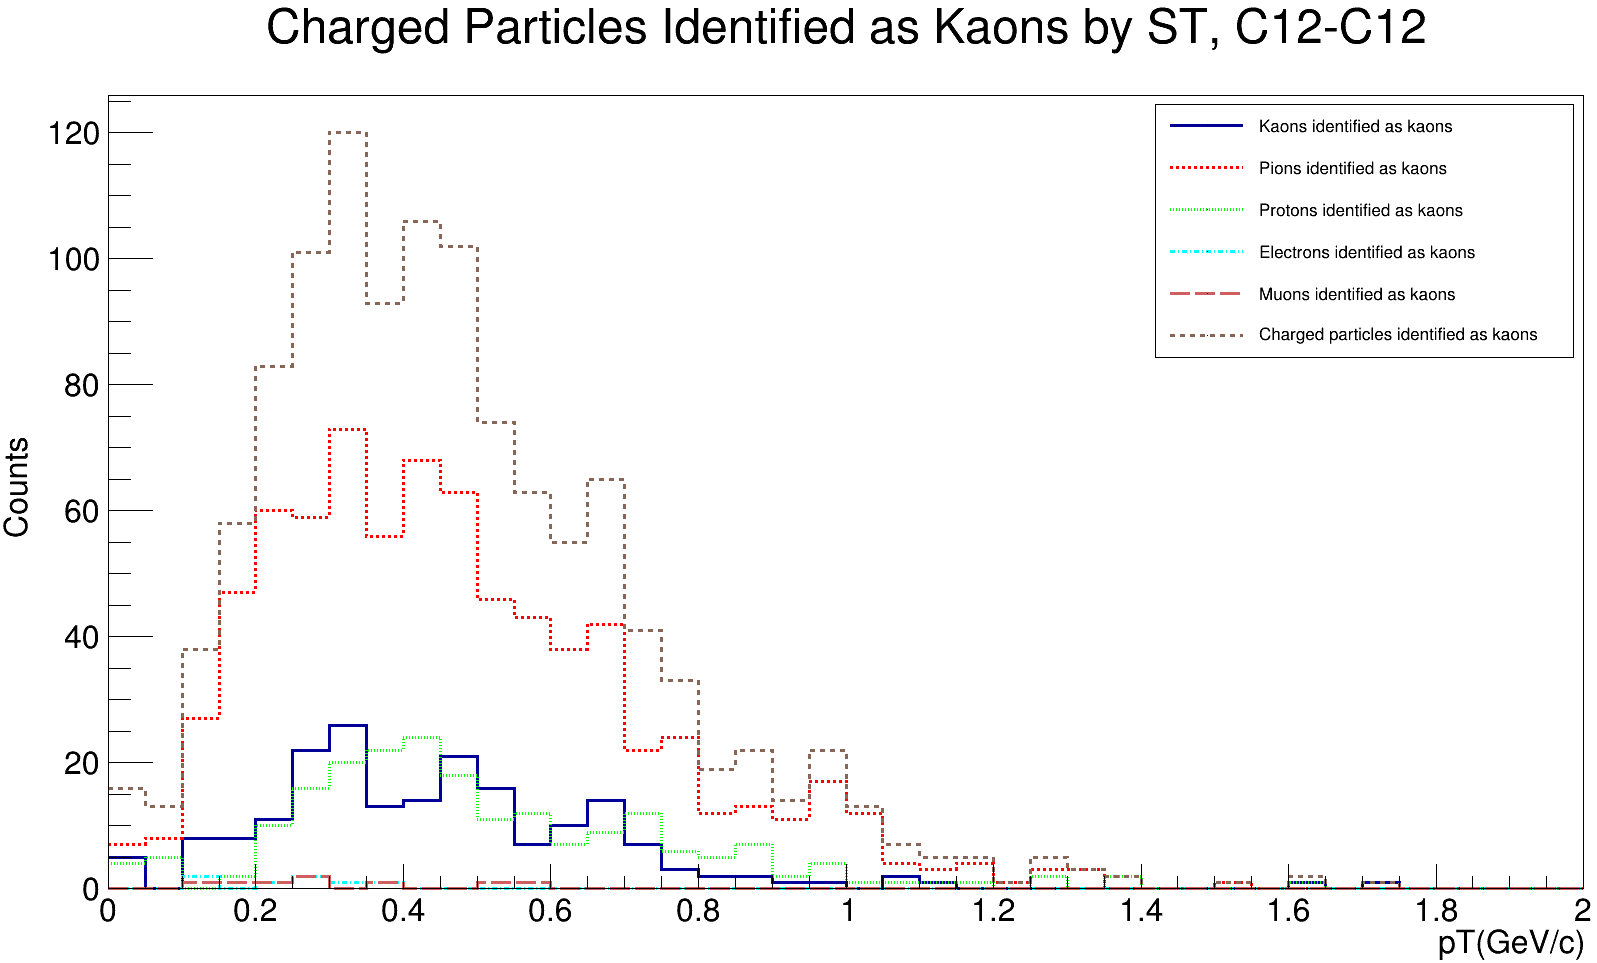
\includegraphics[scale=0.14]{Detector_pT_kaons(st)_C12.png}
\caption{Transverse momentum distribution of charged particles identified as $k^{\pm}$ by ST.}
\label{Detector - Transverse momentum distribution of kaons (ST) C12.}
\end{subfigure}
\caption{Transverse momentum distribution of charged particles identified as $k^{\pm}$ in $^{12}C-{^{12}C}$ collision (Detector level).}
\label{Transverse momentum distribution of charged particles identified as kaons in C12-C12 collision.}
\end{figure*}


\begin{figure*}[h]
\centering
\begin{subfigure}[h]{0.49\textwidth}
\centering
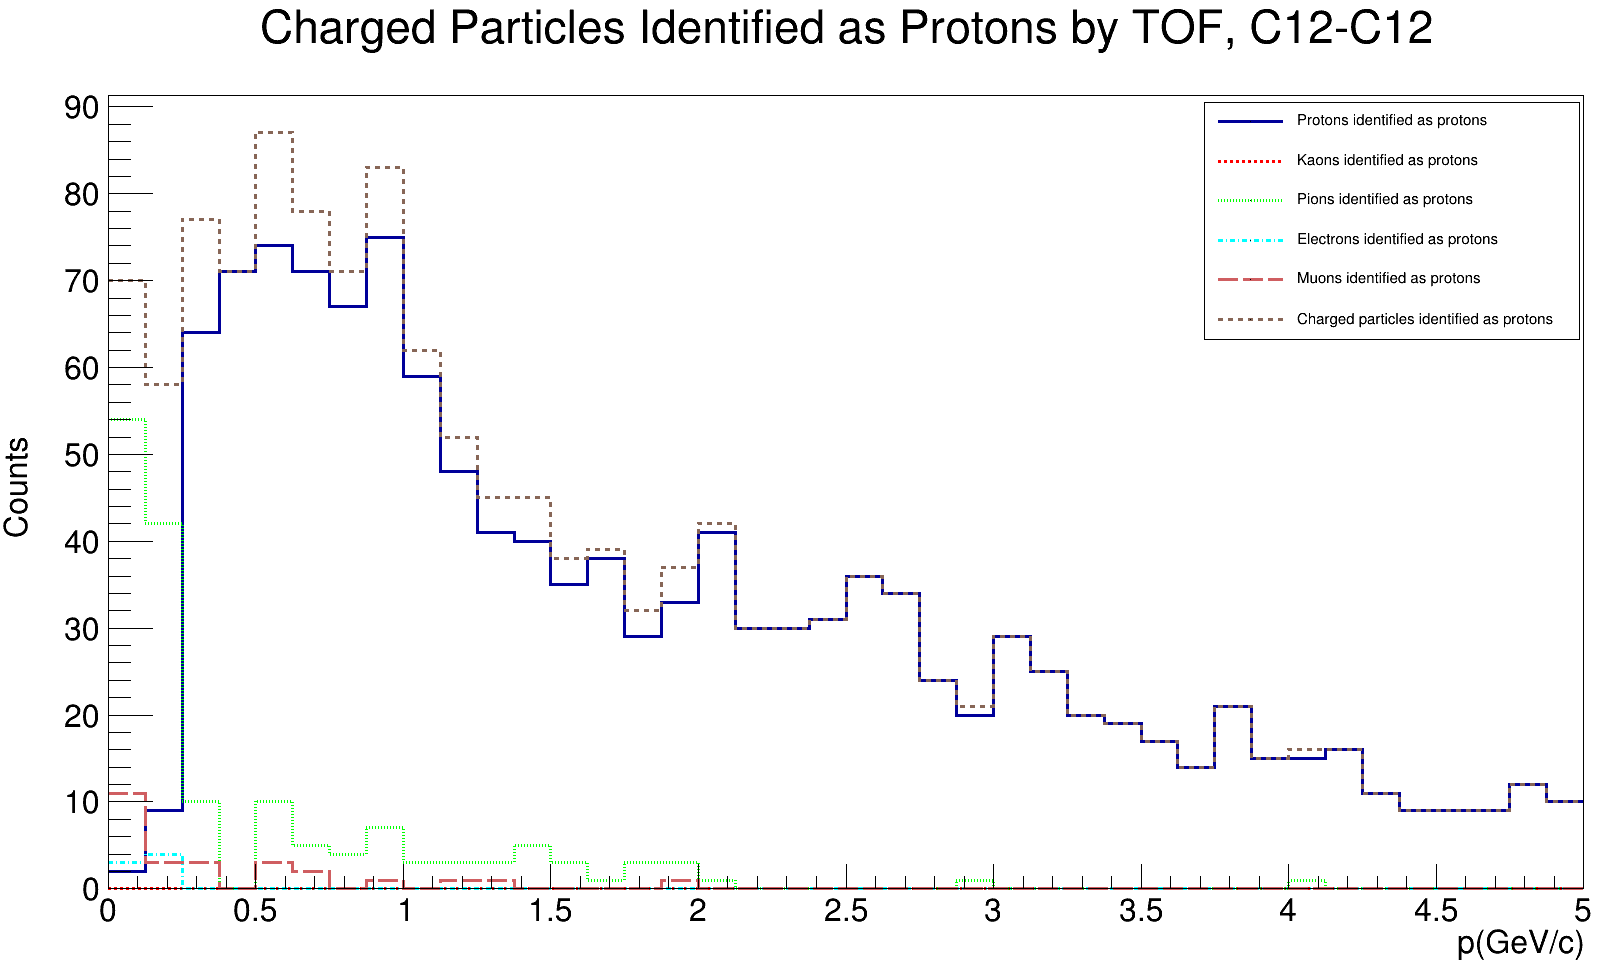
\includegraphics[scale=0.14]{Detector_pToT_protons(tof)_C12.png}
\caption{Total momentum distribution of charged particles identified as $p^{\pm}$ by TOF.}
\label{Detector - Total momentum distribution of protons (TOF) C12.}
\end{subfigure}
\hfill
\begin{subfigure}[h]{0.49\textwidth}
\centering
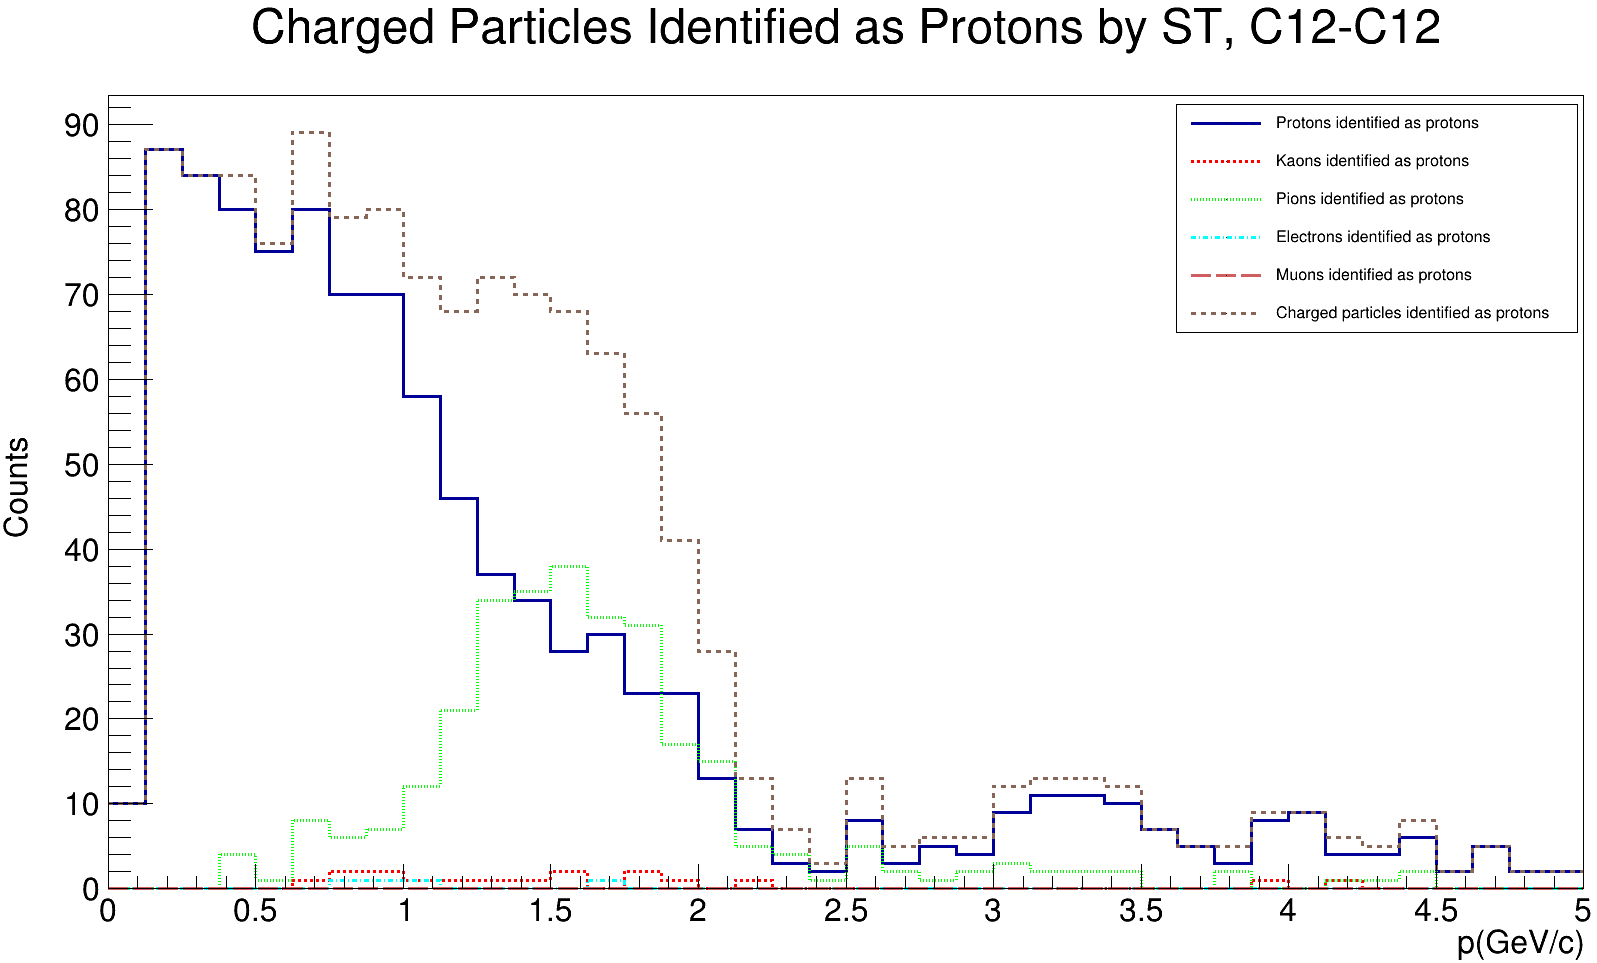
\includegraphics[scale=0.14]{Detector_pToT_protons(st)_C12.png}
\caption{Total momentum distribution of charged particles identified as $p^{\pm}$ by ST.}
\label{Detector - Total momentum distribution of protons (ST) C12.}
\end{subfigure}
\caption{Total momentum distribution of charged particles identified as $p^{\pm}$ in $^{12}C-{^{12}C}$ collision (Detector level).}
\label{Total momentum distribution of charged particles identified as protons in C12-C12 collision.}
\end{figure*}

\begin{figure*}[h]
\centering
\begin{subfigure}[h]{0.49\textwidth}
\centering
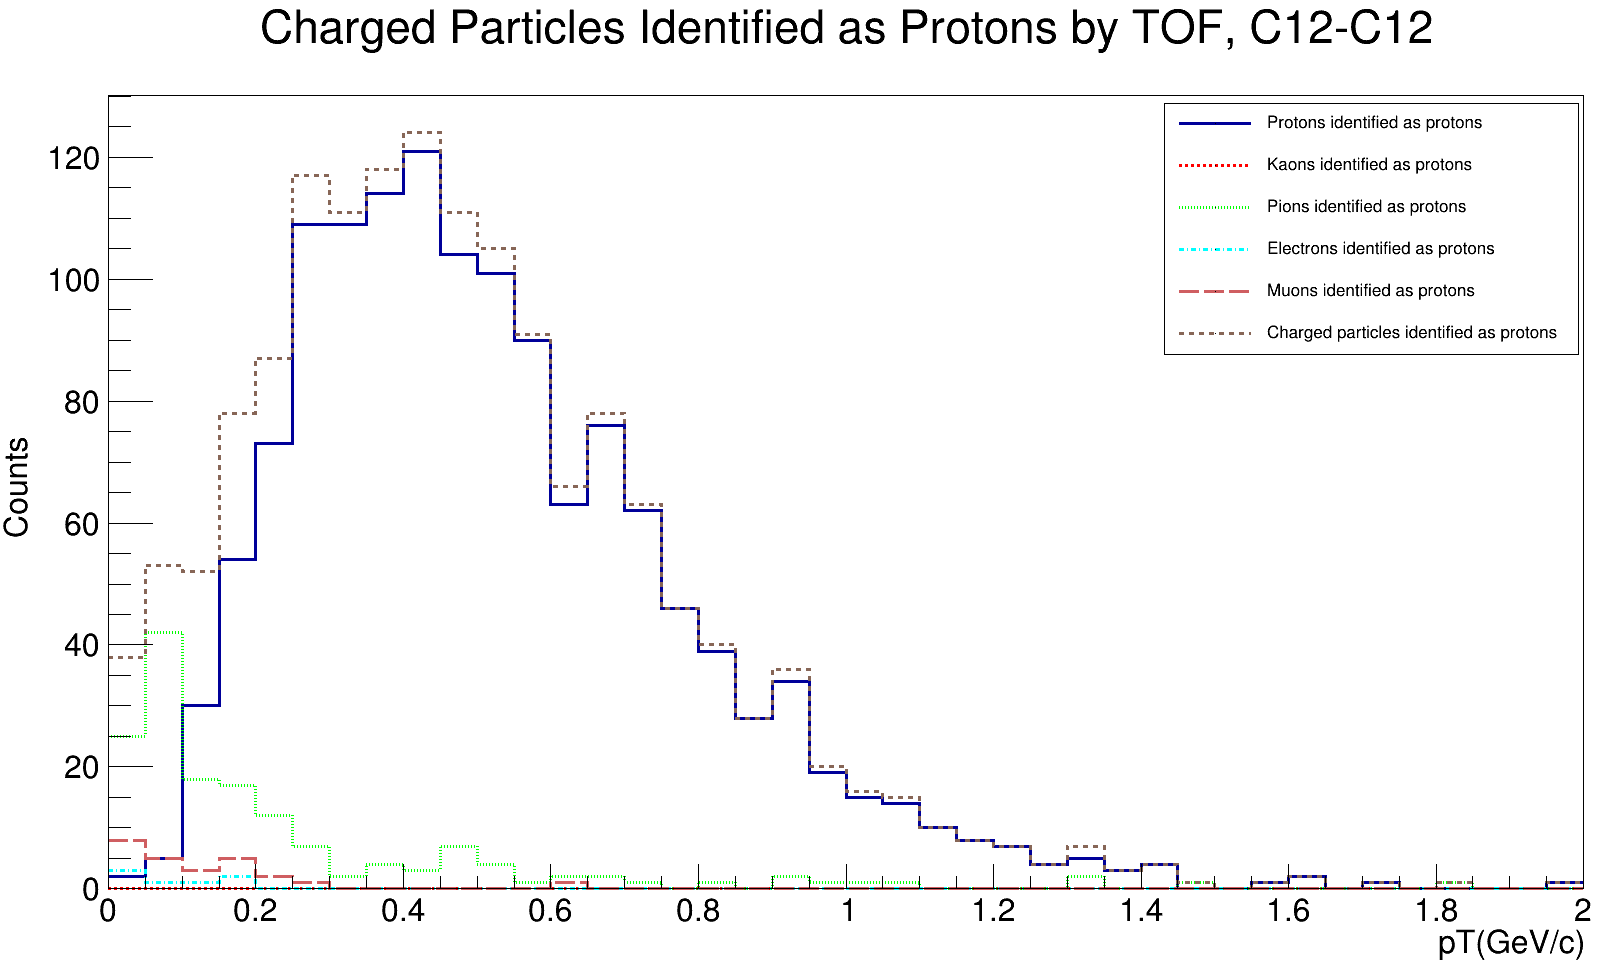
\includegraphics[scale=0.14]{Detector_pT_protons(tof)_C12.png}
\caption{Transverse momentum distribution of charged particles identified as $p^{\pm}$ by TOF.}
\label{Detector - Transverse momentum distribution of protons (TOF) C12.}
\end{subfigure}
\hfill
\begin{subfigure}[h]{0.49\textwidth}
\centering
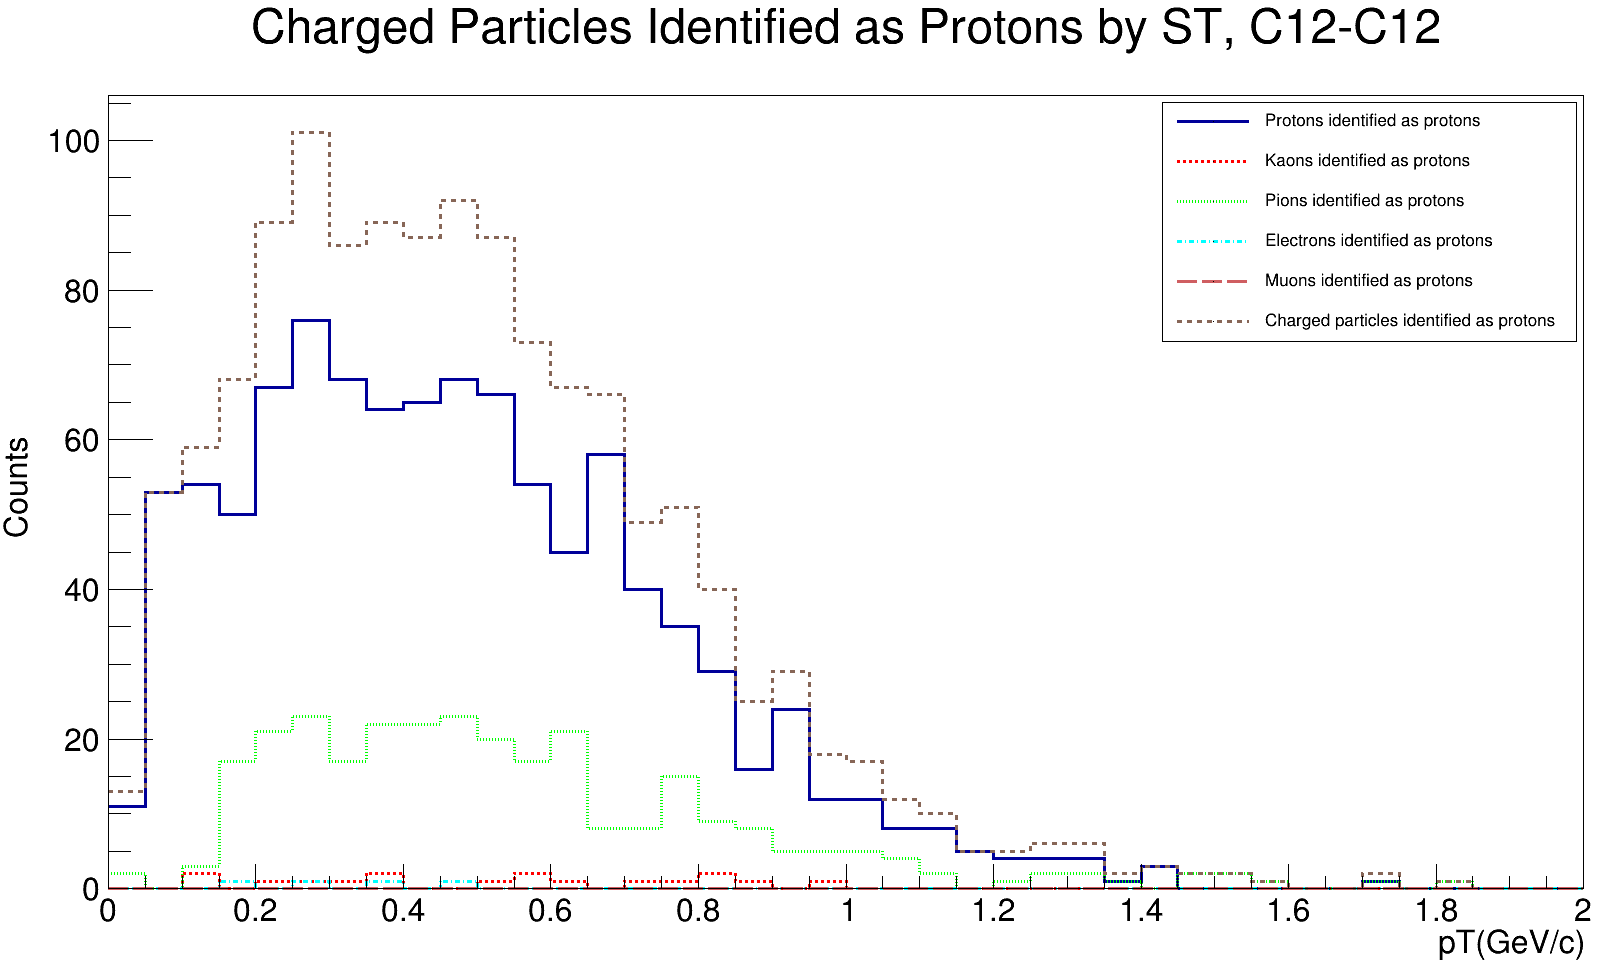
\includegraphics[scale=0.14]{Detector_pT_protons(st)_C12.png}
\caption{Transverse momentum distribution of charged particles identified as $p^{\pm}$ by ST.}
\label{Detector - Transverse momentum distribution of protons (ST) C12.}
\end{subfigure}
\caption{Transverse momentum distribution of charged particles identified as $p^{\pm}$ in $^{12}C-{^{12}C}$ collision (Detector level).}
\label{Transverse momentum distribution of charged particles identified as protons in C12-C12 collision.}
\end{figure*}

\clearpage

%%%%%%%%%%%%%%%%%% End of C12-C12 analysis %%%%%%%%%%%%%%%%%%%%%%%%%%


%%%%%%%%%%%%%%%%%% Strat of Ca40-C40 analysis %%%%%%%%%%%%%%%%%%%%%%%%%

\subsection{DETECTOR LEVEL RESULTS IN $^{40}Ca-{^{40}Ca}$ HEAVY ION COLLISION}
\label{DETECTOR LEVEL RESULTS IN Ca-Ca HEAVY ION COLLISION}
In detector simulation of $^{12}C-{^{12}C}$ heavy ion collision at NICA-SPD, it was observed that the performance of the tracking system (TOF \& ST) for pion identification was very promising. For kaon identification, there were more contaminations and background in momentum spectra recorded by both TOF and ST. However, for proton identification, the performance of ST didn't proved to be as good as that of TOF. The performance of TOF in a specific region ($p > 0.25GeV/c$) showed high level precision $>80\%$. In this section, the goal is to recheck performances of the tracking system by performing detector simulation of $^{40}Ca-{^{40}Ca}$ heavy ion collision at NICA-SPD.

\subsubsection{CHARGED TRACK MULTIPLICITY, $^{40}Ca-{^{40}Ca}$}
\begin{figure}[h]
\centering
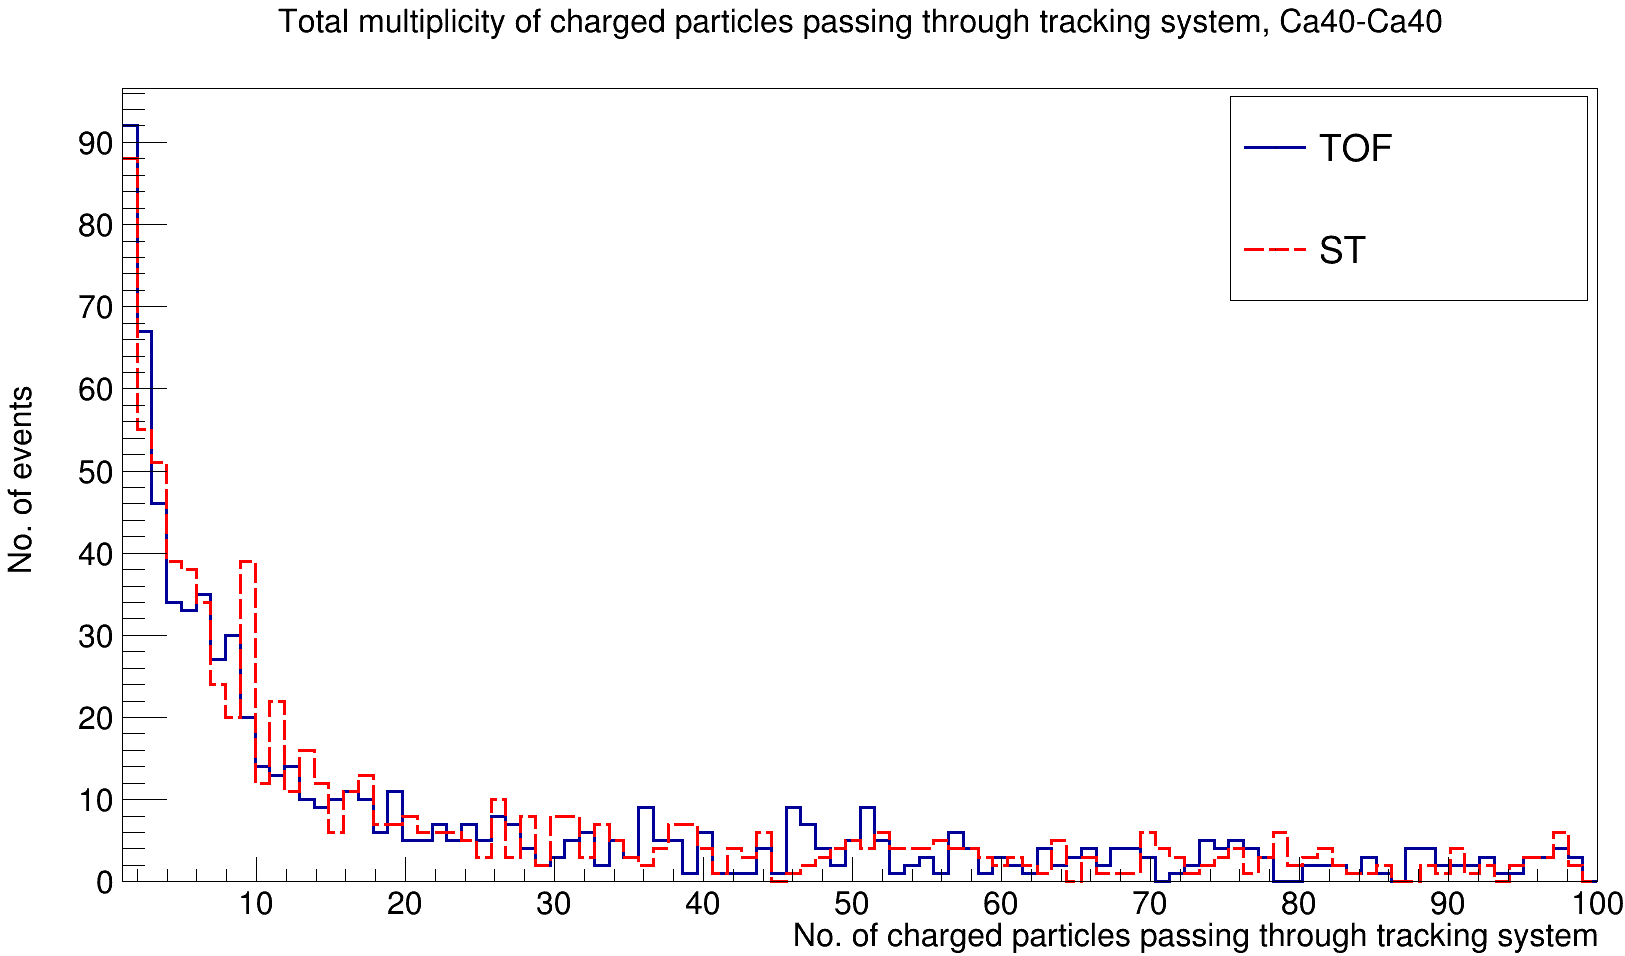
\includegraphics[scale=0.14]{Detector_TotalMultiplicity_Ca40.png}
\caption{Total multiplicity of charged particles passing through tracking system. Red-dashed line is for charged particles passing through ST, and blue line is for charged particles passing through TOF, in $^{40}Ca-{^{40}Ca}$ collision (Detector level).}
\label{Total multiplicity of charged particles passing through tracking system. Red-dashed line is for charged particles passing through ST, and blue line is for charged particles passing through TOF, in Ca40-Ca40 collision (Detector stage).}
\end{figure}
Total multiplicity of charged particles passing through tracking system in simulation of $^{40}Ca-{^{40}Ca}$ collision is shown by Fig.\ref{Total multiplicity of charged particles passing through tracking system. Red-dashed line is for charged particles passing through ST, and blue line is for charged particles passing through TOF, in Ca40-Ca40 collision (Detector stage).}. The X-axis starts from 1 and the reason is explained in sec \ref{CHARGED TRACK MULTIPLICITY, C12-C12}. From this multiplicity plot we come to about the occupancies of the tracking detectors. The detectors identify tracks well for events with less number of reconstructed charged particles. It could be explained well with the help of ST detector. If more than one track passes through a single straw tube at a time, then the signal of both the tracks may not be read properly by the FEE boards. A single straw tube can work more efficiently, if one track passes at one time.

\subsubsection{PION MOMENTUM (p $\&$ pT) SPECTRA, $^{40}Ca-{^{40}Ca}$}
For pion momentum spectra, Fig.\ref{Total momentum distribution of charged particles identified as pions in Ca40-Ca40 collision.}, and Fig.\ref{Transverse momentum distribution of charged particles identified as pions in Ca40-Ca40 collision.} shows the detector level results. The dark blue lines are the correctly identified pions by tracking system while the brown-dashed line represents all charged particles which were identified as pions. In the four figures (\ref{Detector - Total momentum distribution of pions (TOF) Ca40.}, \ref{Detector - Total momentum distribution of pions (ST) Ca40.}, \ref{Detector - Transverse momentum distribution of pions (TOF) Ca40.}, \ref{Detector - Transverse momentum distribution of pions (ST) Ca40.}), it can be seen that the plot of correctly identified pions almost aligns with the plot of  charged particles identified as pions. Also very few other particles have been incorrectly identified as pions by both TOF and ST systems. However, in case of ST, the contamination is slightly more than TOF but the results are promising in both the cases. This reconfirms the high performance of tracking system for pion identification during heavy ion collision at SPD.      

\subsubsection{KAON MOMENTUM (p $\&$ pT) SPECTRA, $^{40}Ca-{^{40}Ca}$}
\label{KAON MOMENTUM (p and pT) SPECTRA, Ca40-Ca40}
For kaon momentum spectra, the detector level results are shown by Fig.\ref{Total momentum distribution of charged particles identified as kaons in Ca40-Ca40 collision.}, and \ref{Transverse momentum distribution of charged particles identified as kaons in Ca40-Ca40 collision.}. Unlike the high performance shown by tracking system in pion identification, in this case the performance of tracking system seems very low. The correctly identified kaons (blue line) are quite less as compared to all charged particles identified as kaons (brown line). Thus, the performance of tracking system for kaon identification during heavy ion collisions seems very low. It's interesting to note that in TOF system (for $p < 0.45$, and $pT < 0.35$, see Fig.\ref{Detector - Total momentum distribution of kaons (TOF) Ca40.}, \ref{Detector - Transverse momentum distribution of kaons (TOF) Ca40.}) and in ST system (for $p > 0.6$, and $pT > 0$, see Fig.\ref{Detector - Total momentum distribution of kaons (ST) Ca40.}, \ref{Detector - Transverse momentum distribution of kaons (ST) Ca40.}) more pions were incorrectly identified as kaons than the true kaons itself. Hence, the contamination is very high is this case.

\subsubsection{PROTON MOMENTUM (p $\&$ pT) SPECTRA, $^{40}Ca-{^{40}Ca}$}
\label{PROTON MOMENTUM (p and pT) SPECTRA, Ca40-Ca40}  
Total $\&$ transverse momentum distribution of protons were analysed at detector level (see Fig.\ref{Total momentum distribution of charged particles identified as protons in Ca40-Ca40 collision.}, \& \ref{Transverse momentum distribution of charged particles identified as protons in Ca40-Ca40 collision.}) for Ca-Ca heavy-ion collision. Likewise in previous collision, it was observed here too that in TOF system (for $p < 0.25$, or $pT < 0.1$, see Fig.\ref{Detector - Total momentum distribution of protons (TOF) Ca40.}, \ref{Detector - Transverse momentum distribution of protons (TOF) Ca40.}) and in ST system (for $0.5 < p < 2.5$, and $0.15 < pT < 0.85$, see Fig.\ref{Detector - Total momentum distribution of protons (ST) Ca40.}, \ref{Detector - Transverse momentum distribution of protons (ST) Ca40.}) more pions were incorrectly identified as protons than the true protons itself. This shows that the contamination in these regions were more. However, above a certain value of momentum, the performance of TOF in proton identification was much better than ST. For $p > 0.25$, the TOF system showed high level of precision greater than 80\% while the performance of ST was not up to to the mark. Hence, it is rechecked using two different, heavy ion collisions that ``Proton identification can be done using TOF only for $p > 0.25 GeV/c$". See section \ref{PROTON MOMENTUM (p and pT) SPECTRA, C12-C12} for the first collision. More about the performance and precision shown by the tracking systems for different charged particle identification have been explained in sec \ref{PRECISION GRAPH OF MOMENTUM SPECTRA}.  

\section{PRECISION GRAPH OF MOMENTUM SPECTRA}
\label{PRECISION GRAPH OF MOMENTUM SPECTRA}
The momentum spectra of charged pions, kaons, and protons at detector stage were used to procure precision graphs, which provides two important informations. First, the performance of the tracking system, and second, the feasibility of studies for hadron formation effects at first stage of NICA-SPD. The precision was calculated using the ratio - number of correctly identified particles of a certain type to the total number of particles identified as a certain type. For example, for pion momentum spectra, precision would be, number of correctly identified pions to the total number of charged particles identified as pions.

In pion spectra precision, it was observed that the TOF system makes precise identification of pions in entire momentum range upto 2 GeV/c for both C-C and Ca-Ca collisions. The precision recorded by this system was above 90\% as seen from the figures \ref{Pion spectra precision, C12.}, \ref{Pion spectra precision, Ca40.}. However, the ST system makes precise pion identification upto 1.2 GeV/c. After this, fluctuations were observed and precision decreased even below 50\% in case of Ca-Ca. The reason of sudden decrease in precision after 1.2  GeV/c for ST is that the number of correctly identified pions (with $p > 1.2$) crossing ST decreased in large extent as compared to true pions reconstructed. Hence, even a small level of misidentification can lead to large drop in precision. So, the measurement of pion spectra seems easily possible. Hence, hadron formation effects can be studied using pion spectra in heavy ion collision at first stage of NICA-SPD.

Identification of kaons by tracking system in both the collisions doesn't seems to be promising as there were many contaminations, see Fig.\ref{Kaon spectra precision, C12.}, \ref{Kaon spectra precision, Ca40.}. There were regions of momentum when more pions were incorrectly identified as kaons than the true kaons itself (see sec \ref{KAON MOMENTUM (p and pT) SPECTRA, C12-C12} \& \ref{KAON MOMENTUM (p and pT) SPECTRA, Ca40-Ca40}). Thus, measurement of kaon spectra doesn't seems to be possible and so the hadron formation effects can't be studied using kaon spectra in heavy ion collision at SPD-first stage.

The proton spectra precision is shown by Fig.\ref{Proton spectra precision, C12}, \ref{Proton spectra precision, Ca40}. It was observed that the precision recorded by ST in proton identification has many crest and trough.

\clearpage


%%%%%%%%%%%%%%%%% Momentum (p & pT) Distribution Ca40-C40 %%%%%%%%%%%%%%

\begin{figure*}[h]
\centering
\begin{subfigure}[h]{0.49\textwidth}
\centering
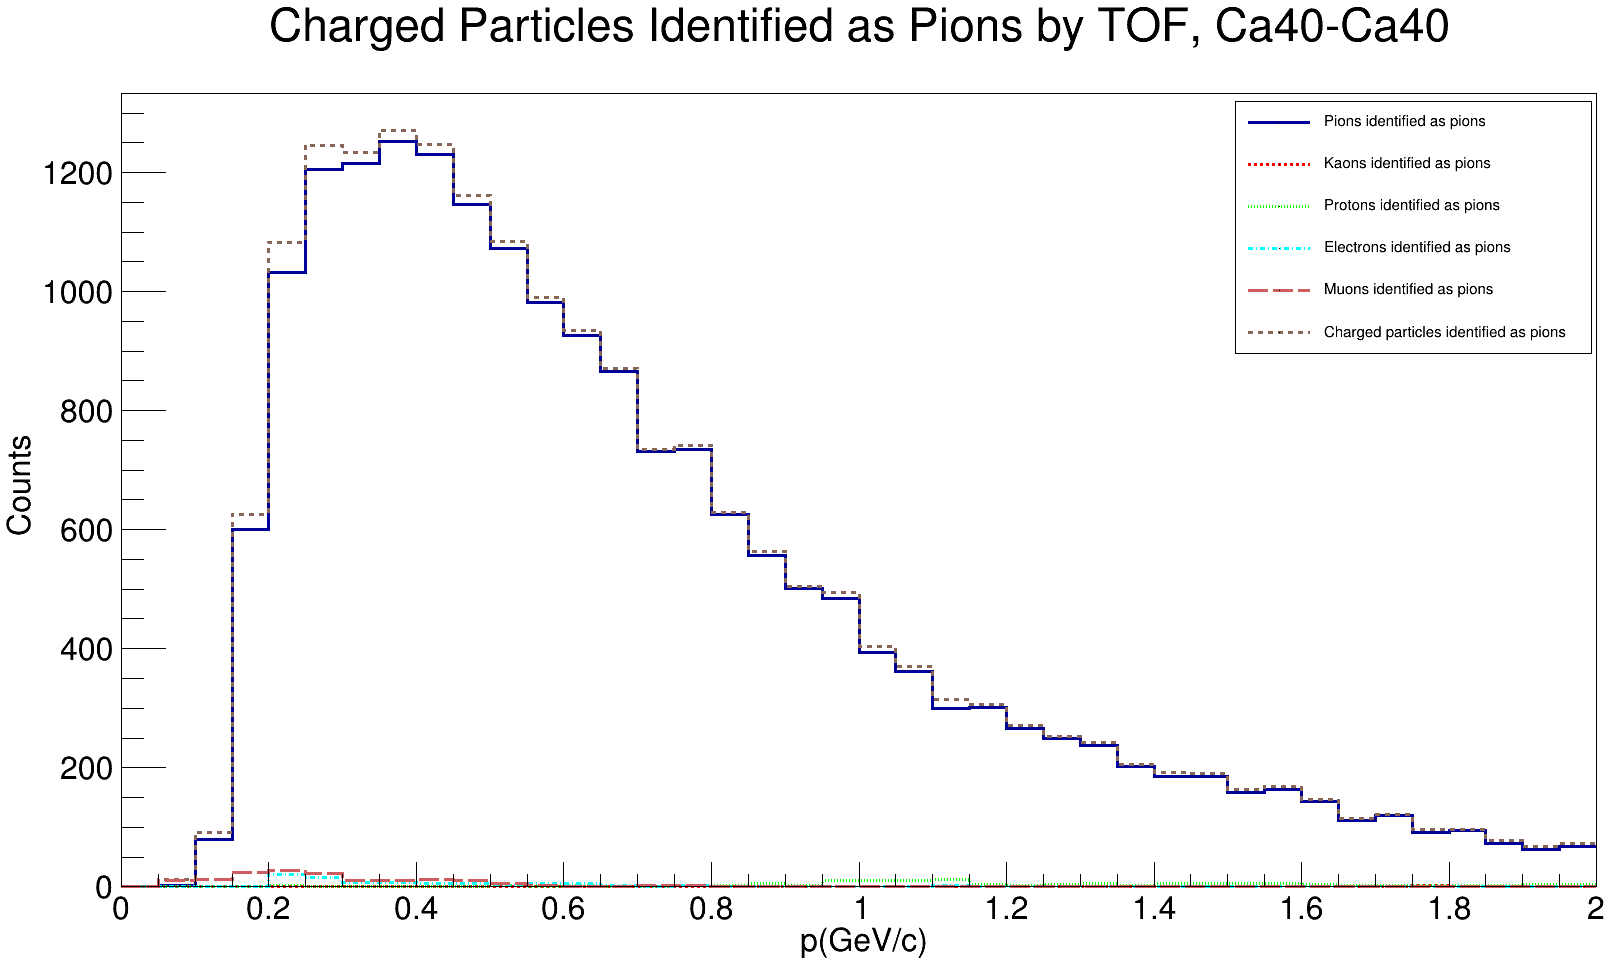
\includegraphics[scale=0.14]{Detector_pToT_pions(tof)_Ca.png}
\caption{Total momentum distribution of charged particles identified as $\pi^{\pm}$ by TOF.}
\label{Detector - Total momentum distribution of pions (TOF) Ca40.}
\end{subfigure}
\hfill
\begin{subfigure}[h]{0.49\textwidth}
\centering
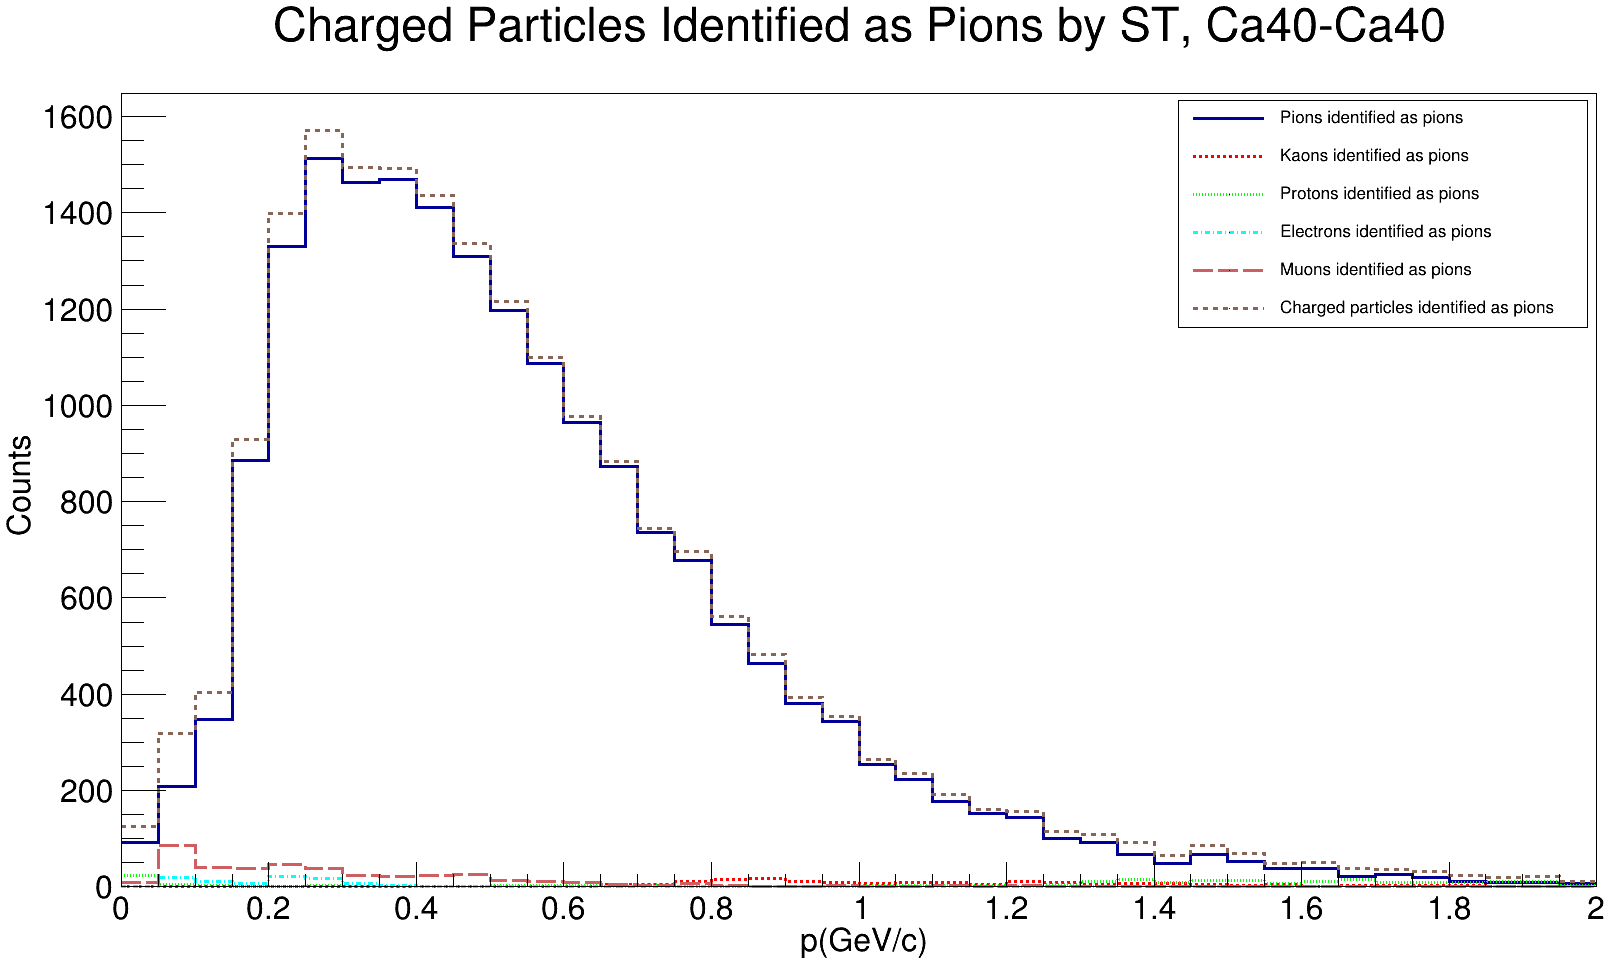
\includegraphics[scale=0.14]{Detector_pToT_pions(st)_Ca.png}
\caption{Total momentum distribution of charged particles identified as $\pi^{\pm}$ by ST.}
\label{Detector - Total momentum distribution of pions (ST) Ca40.}
\end{subfigure}
\caption{Total momentum distribution of charged particles identified as $\pi^{\pm}$ in $^{40}Ca-{^{40}Ca}$ collision (Detector level).}
\label{Total momentum distribution of charged particles identified as pions in Ca40-Ca40 collision.}
\end{figure*}

\begin{figure*}[h]
\centering
\begin{subfigure}[h]{0.49\textwidth}
\centering
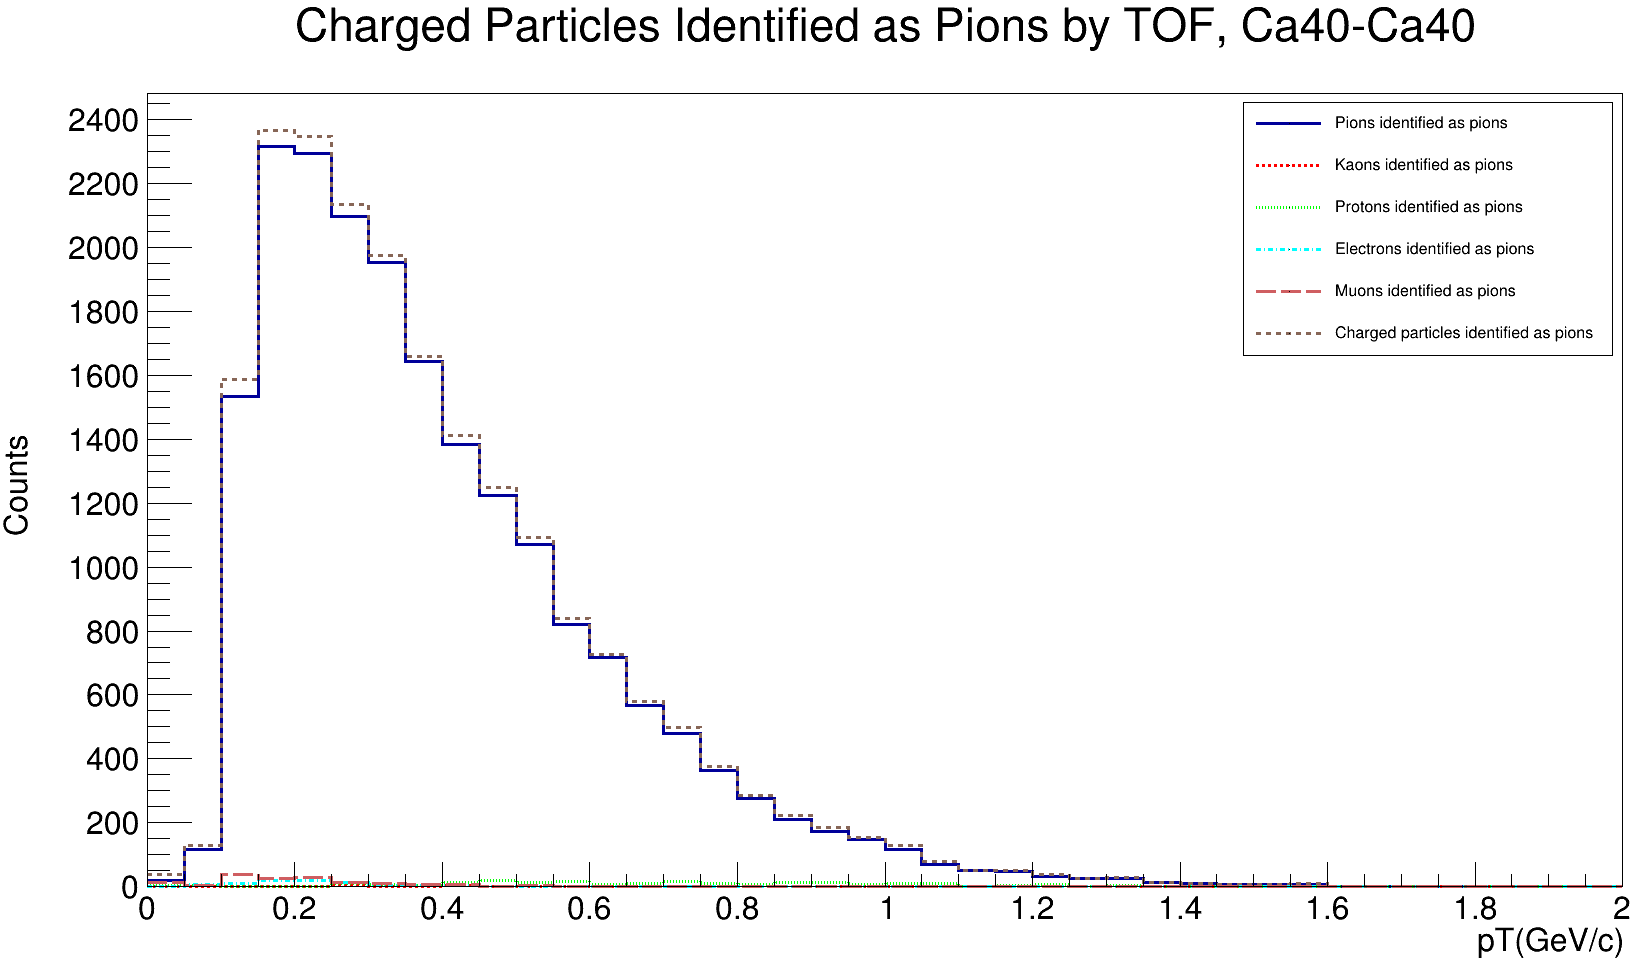
\includegraphics[scale=0.14]{Detector_pT_pions(tof)_Ca.png}
\caption{Transverse momentum distribution of charged particles identified as $\pi^{\pm}$ by TOF.}
\label{Detector - Transverse momentum distribution of pions (TOF) Ca40.}
\end{subfigure}
\hfill
\begin{subfigure}[h]{0.49\textwidth}
\centering
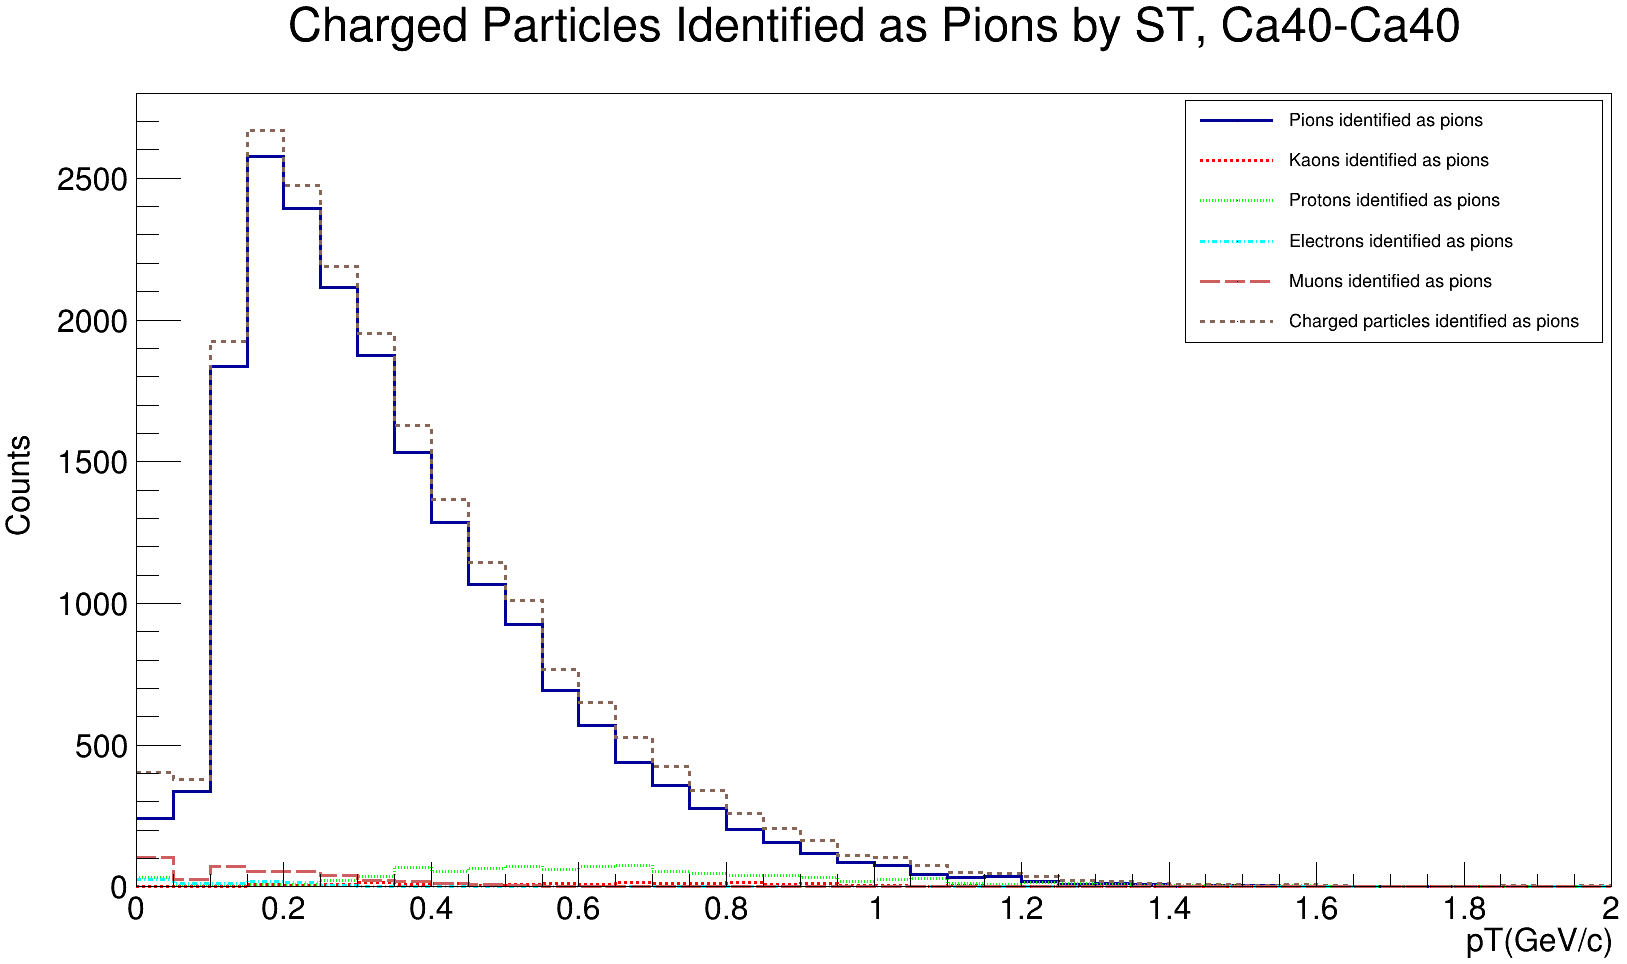
\includegraphics[scale=0.14]{Detector_pT_pions(st)_Ca.png}
\caption{Transverse momentum distribution of charged particles identified as $\pi^{\pm}$ by ST.}
\label{Detector - Transverse momentum distribution of pions (ST) Ca40.}
\end{subfigure}
\caption{Transverse momentum distribution of charged particles identified as $\pi^{\pm}$ in $^{40}Ca-{^{40}Ca}$ collision (Detector level).}
\label{Transverse momentum distribution of charged particles identified as pions in Ca40-Ca40 collision.}
\end{figure*}


\begin{figure*}[h]
\centering
\begin{subfigure}[h]{0.49\textwidth}
\centering
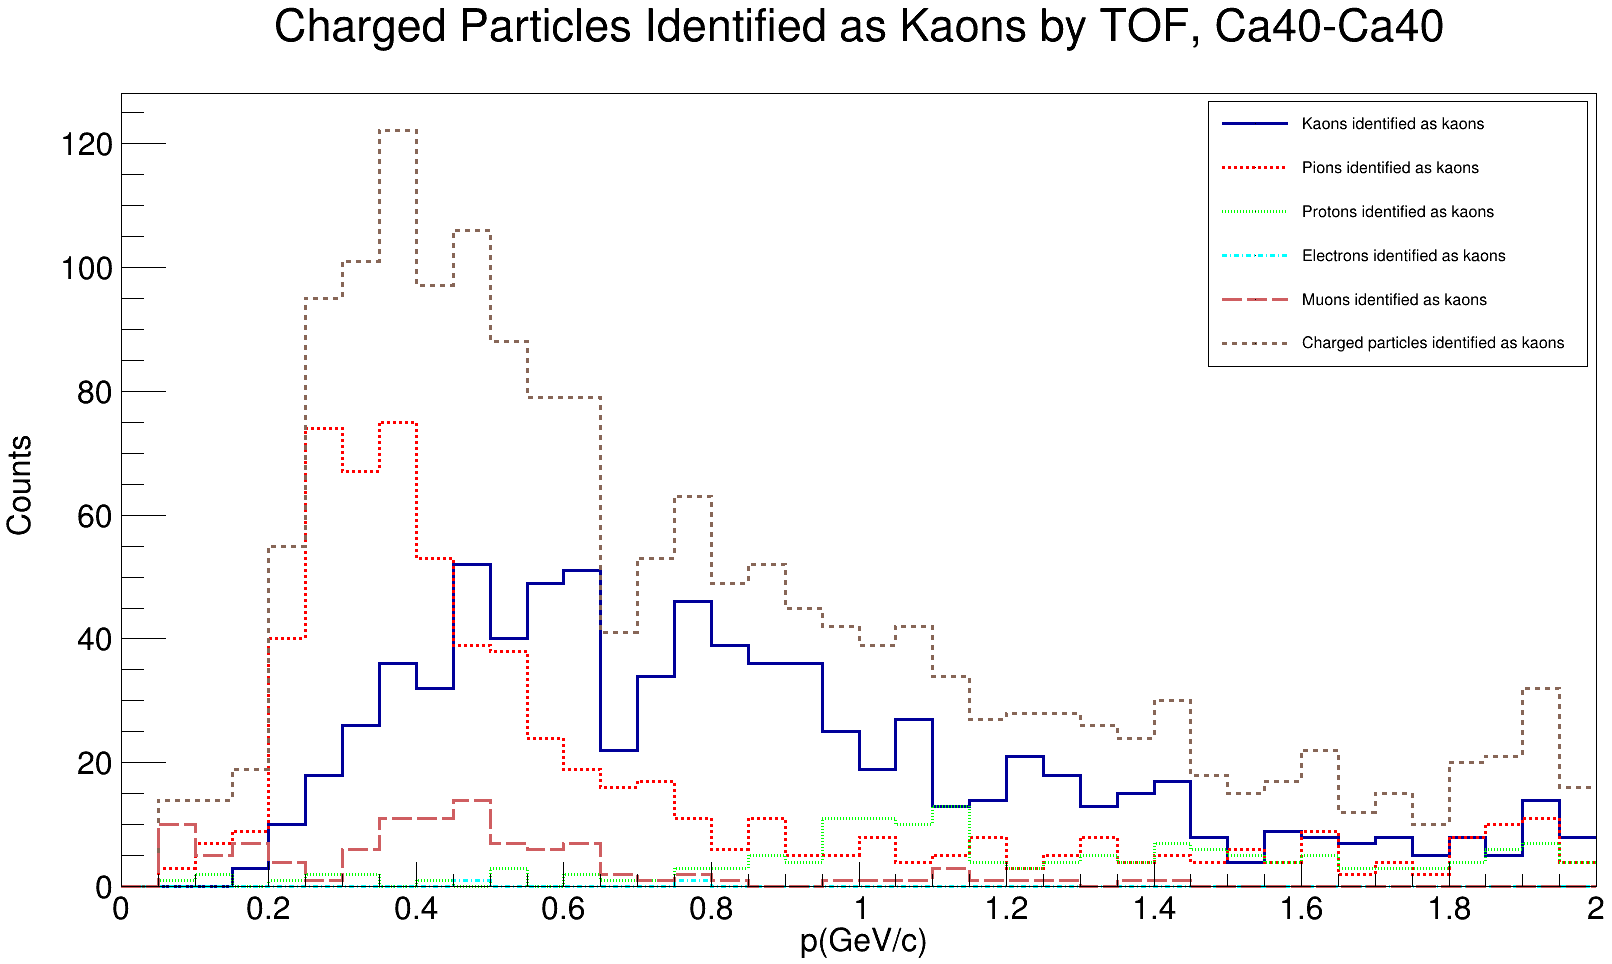
\includegraphics[scale=0.14]{Detector_pToT_kaons(tof)_Ca.png}
\caption{Total momentum distribution of charged particles identified as $k^{\pm}$ by TOF.}
\label{Detector - Total momentum distribution of kaons (TOF) Ca40.}
\end{subfigure}
\hfill
\begin{subfigure}[h]{0.49\textwidth}
\centering
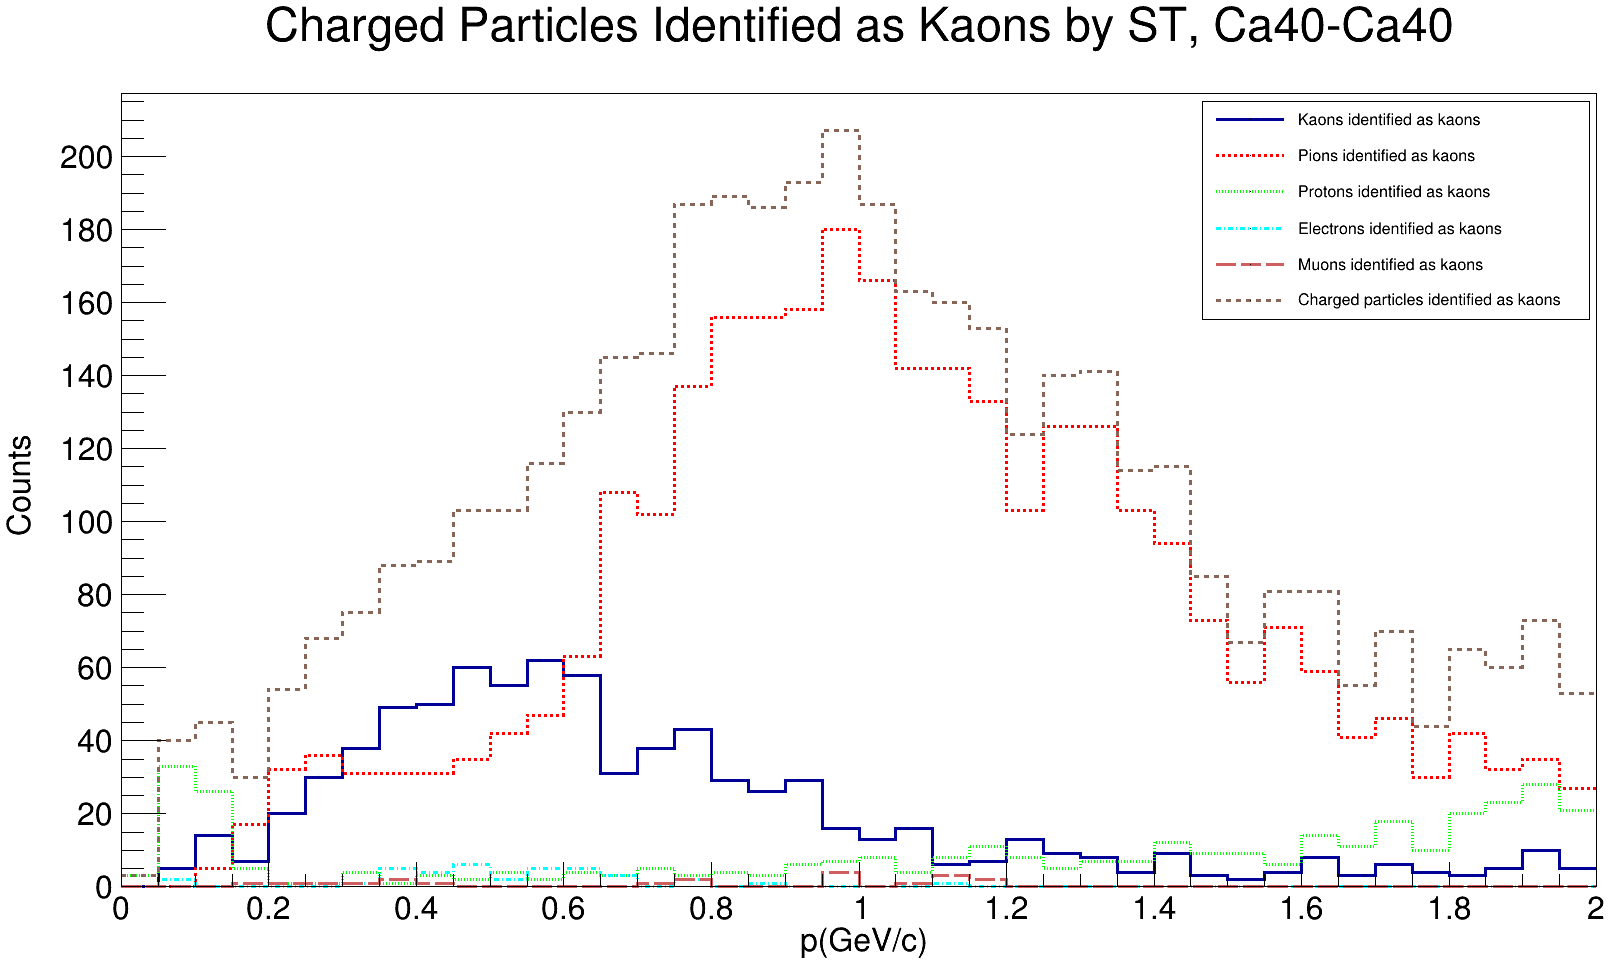
\includegraphics[scale=0.14]{Detector_pToT_kaons(st)_Ca.png}
\caption{Total momentum distribution of charged particles identified as $k^{\pm}$ by ST.}
\label{Detector - Total momentum distribution of kaons (ST) Ca40.}
\end{subfigure}
\caption{Total momentum distribution of charged particles identified as $k^{\pm}$ in $^{40}Ca-{^{40}Ca}$ collision (Detector level).}
\label{Total momentum distribution of charged particles identified as kaons in Ca40-Ca40 collision.}
\end{figure*}

\begin{figure*}[h]
\centering
\begin{subfigure}[h]{0.49\textwidth}
\centering
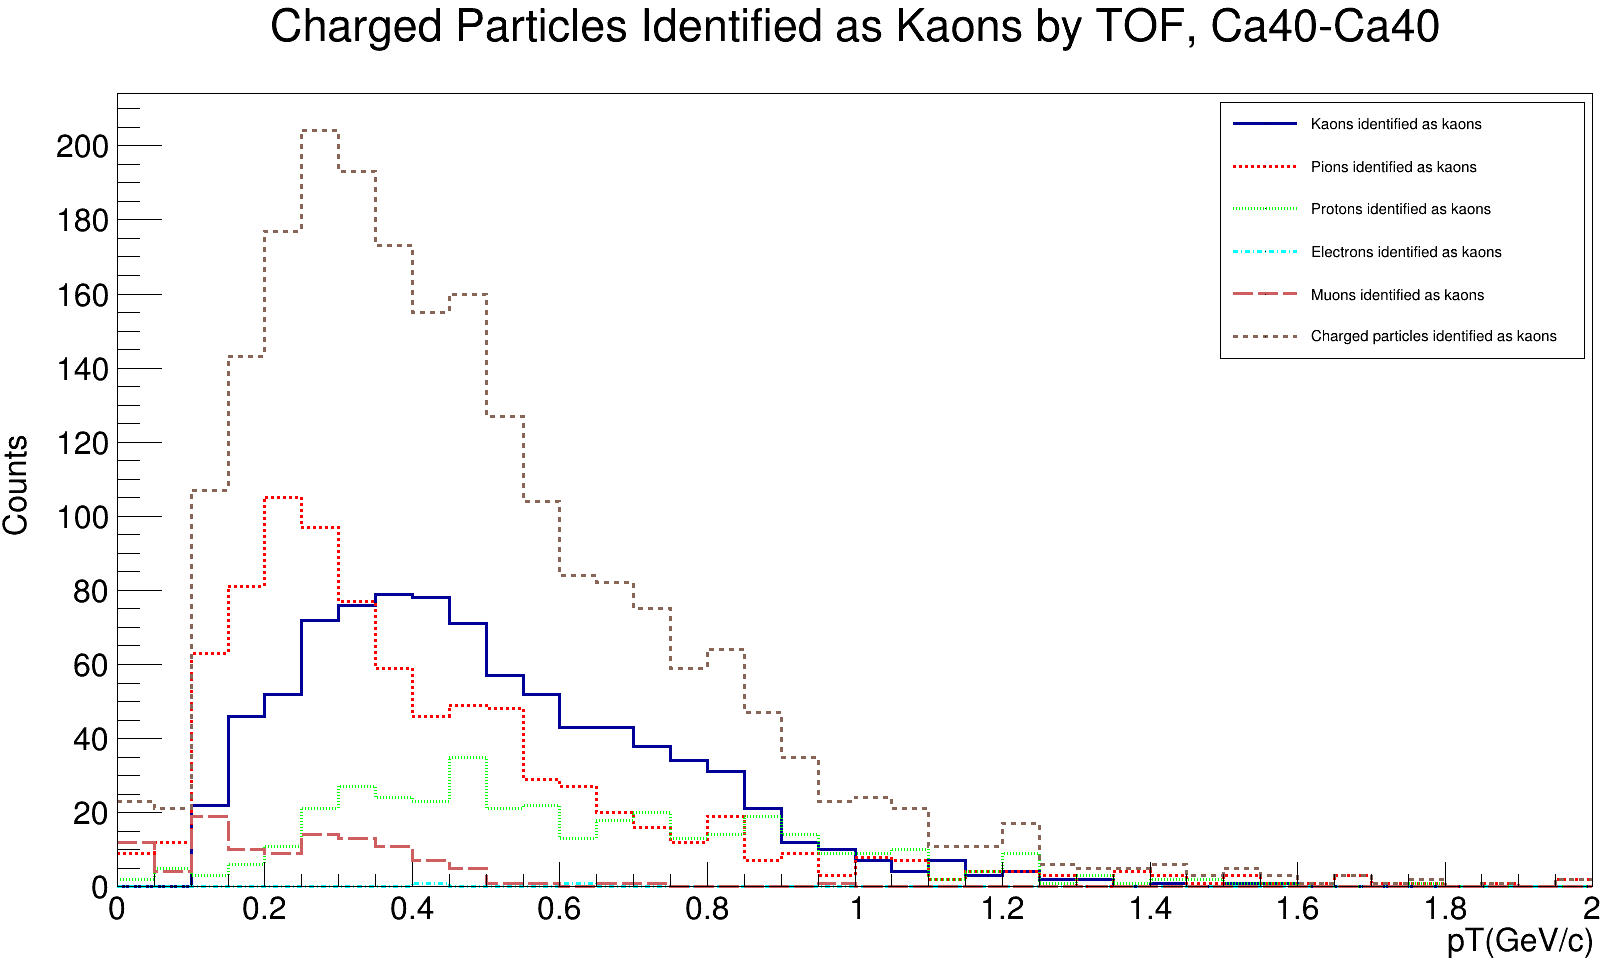
\includegraphics[scale=0.14]{Detector_pT_kaons(tof)_Ca.png}
\caption{Transverse momentum distribution of charged particles identified as $k^{\pm}$ by TOF.}
\label{Detector - Transverse momentum distribution of kaons (TOF) Ca40.}
\end{subfigure}
\hfill
\begin{subfigure}[h]{0.49\textwidth}
\centering
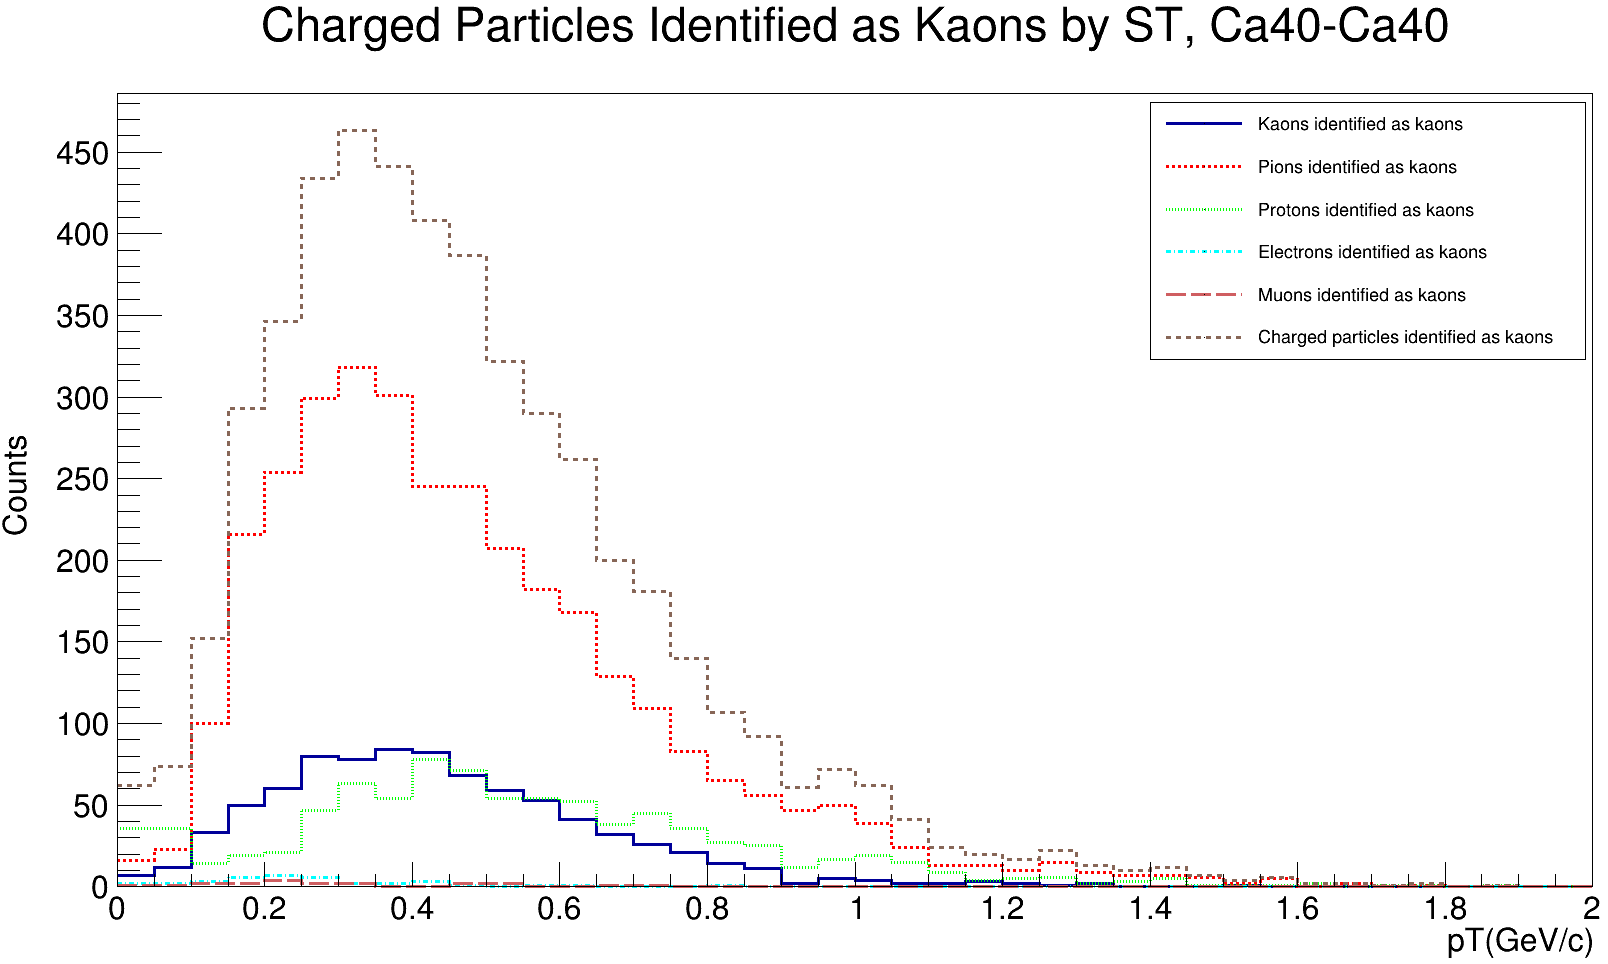
\includegraphics[scale=0.14]{Detector_pT_kaons(st)_Ca.png}
\caption{Transverse momentum distribution of charged particles identified as $k^{\pm}$ by ST.}
\label{Detector - Transverse momentum distribution of kaons (ST) Ca40.}
\end{subfigure}
\caption{Transverse momentum distribution of charged particles identified as $k^{\pm}$ in $^{40}Ca-{^{40}Ca}$ collision (Detector level).}
\label{Transverse momentum distribution of charged particles identified as kaons in Ca40-Ca40 collision.}
\end{figure*}


\begin{figure*}[h]
\centering
\begin{subfigure}[h]{0.49\textwidth}
\centering
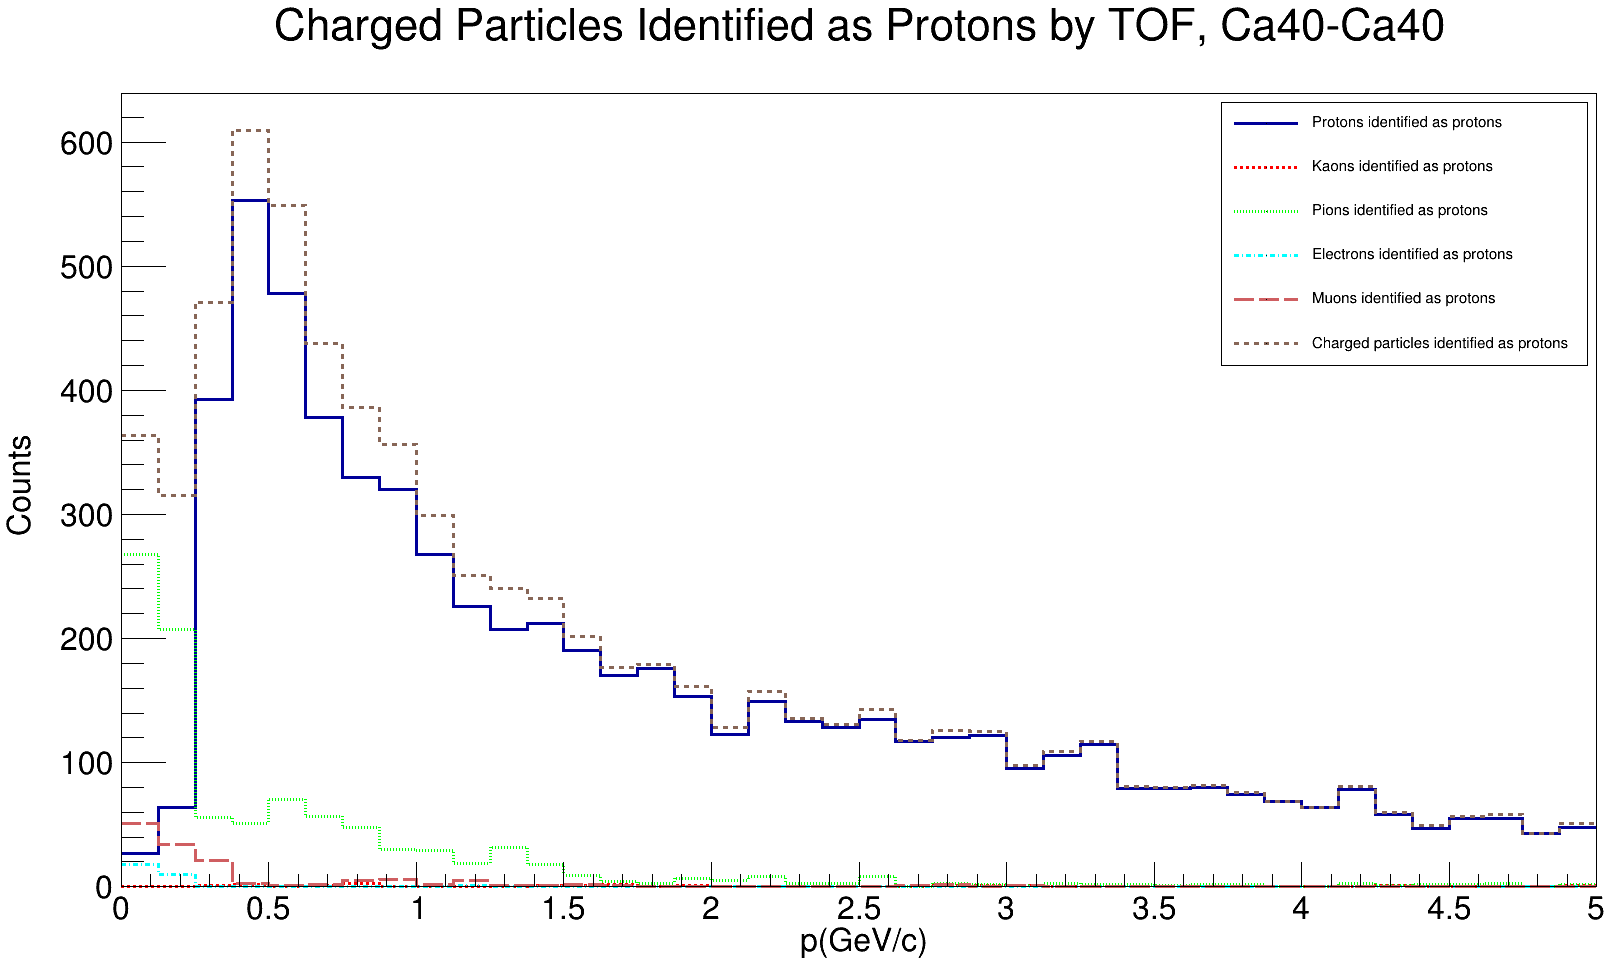
\includegraphics[scale=0.14]{Detector_pToT_protons(tof)_Ca.png}
\caption{Total momentum distribution of charged particles identified as $p^{\pm}$ by TOF.}
\label{Detector - Total momentum distribution of protons (TOF) Ca40.}
\end{subfigure}
\hfill
\begin{subfigure}[h]{0.49\textwidth}
\centering
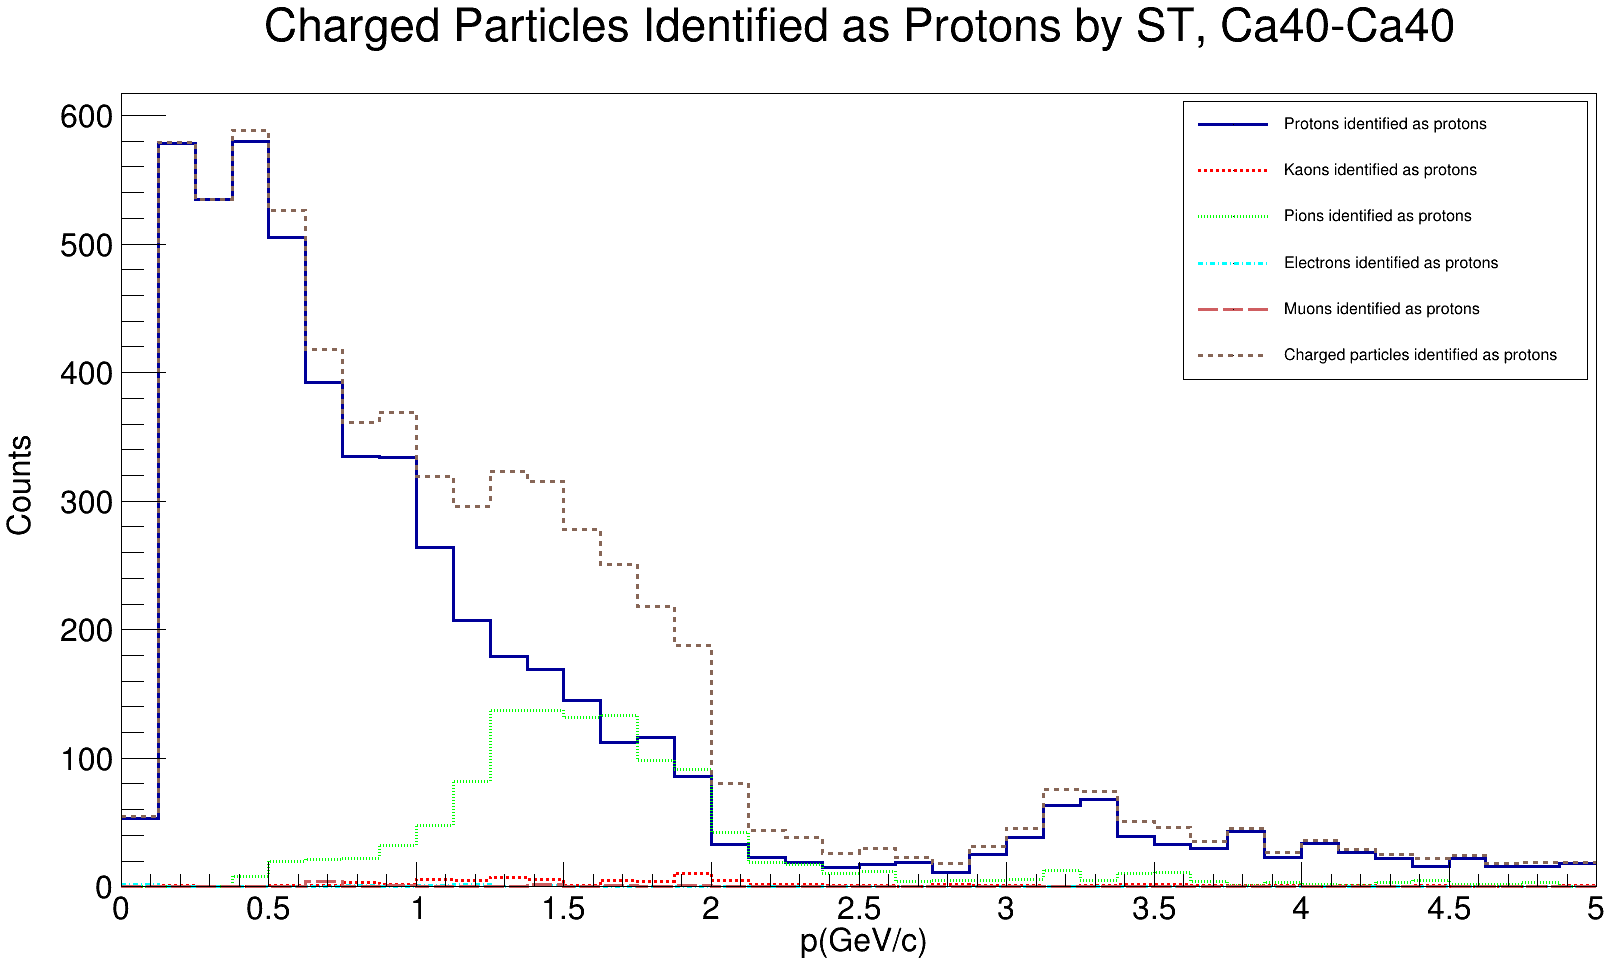
\includegraphics[scale=0.14]{Detector_pToT_protons(st)_Ca.png}
\caption{Total momentum distribution of charged particles identified as $p^{\pm}$ by ST.}
\label{Detector - Total momentum distribution of protons (ST) Ca40.}
\end{subfigure}
\caption{Total momentum distribution of charged particles identified as $p^{\pm}$ in $^{40}Ca-{^{40}Ca}$ collision (Detector level).}
\label{Total momentum distribution of charged particles identified as protons in Ca40-Ca40 collision.}
\end{figure*}

\begin{figure*}[h]
\centering
\begin{subfigure}[h]{0.49\textwidth}
\centering
\includegraphics[scale=0.1398]{Detector_pT_protons(tof)_Ca.png}
\caption{Transverse momentum distribution of charged particles identified as $p^{\pm}$ by TOF.}
\label{Detector - Transverse momentum distribution of protons (TOF) Ca40.}
\end{subfigure}
\hfill
\begin{subfigure}[h]{0.49\textwidth}
\centering
\includegraphics[scale=0.1398]{Detector_pT_protons(st)_Ca.png}
\caption{Transverse momentum distribution of charged particles identified as $p^{\pm}$ by ST.}
\label{Detector - Transverse momentum distribution of protons (ST) Ca40.}
\end{subfigure}
\caption{Transverse momentum distribution of charged particles identified as $p^{\pm}$ in $^{40}Ca-{^{40}Ca}$ collision (Detector level).}
\label{Transverse momentum distribution of charged particles identified as protons in Ca40-Ca40 collision.}
\end{figure*}

\clearpage

%%%%%%%%%%%%%%%%%%%%%% END OF Ca40-Ca40 analysis %%%%%%%%%%%%%%%%%%%%%%%%%%%%%%%%%%%%%%%%%


%%%%%%%%%%%%%%%% Precision graph for C12-C12 %%%%%%%%%%%%%%%%%%%%%

\begin{table*}
\begin{tabular}{|c|c|c|}
\hline
Type of particle identification & Purity recorded by TOF & Purity recorded by ST \\
\hline
\hline
$\pi^{\pm}$ identification & $>90\%$ & $>90\%$ for $(p < 1.2GeV/c)$ \\
\hline
$k^{\pm}$ identification & Fluctuating & Fluctuating \\
\hline
$p^{\pm}$ identification & $>80\%$ for $(p > 0.25GeV/c)$ & Fluctuating \\
\hline
\end{tabular}
\captionof{table}{Precision of momentum spectra recorded by tracking systems.}
\label{Precision of momentum spectra recorded by tracking systems.} 
\end{table*}

\begin{figure}[H]
\centering
\begin{subfigure}[h]{0.49\textwidth}
\centering
\includegraphics[scale=0.14]{PionSpectraPrecision_C12.png}
\caption{$\pi^{\pm}$ spectra precision.}
\label{Pion spectra precision, C12.}
\end{subfigure}
\par
\vspace{1.3cm}
\begin{subfigure}[h]{0.49\textwidth}
\centering
\includegraphics[scale=0.14]{KaonSpectraPrecision_C12.png}
\caption{$k^{\pm}$ spectra precision.}
\label{Kaon spectra precision, C12.}
\end{subfigure}
\par
\vspace{1.3cm}
\begin{subfigure}[h]{0.49\textwidth}
\centering
\includegraphics[scale=0.14]{ProtonSpectraPrecision_C12.png}
\caption{$p^{\pm}$ spectra precision.}
\label{Proton spectra precision, C12}
\end{subfigure}
\caption{Precision graphs of $\pi^{\pm}, k^{\pm}$ $\&$ $p^{\pm}$ in $^{12}C-{^{12}C}$ collision. Red line and blue line indicates precision in pion spectra recorded by ionization losses and TOF information respectively.}
\label{Precision graphs of pions, kaons, and protons in C12-C12 collision. Red line and blue line shows precision in pion spectra recorded by ST, and TOF respectively.}
\vspace{2.5cm}
\end{figure}

%%%%%%%%%%%%%%%% Precision graph for Ca40-Ca40 %%%%%%%%%%%%%%%%%%%%%

\begin{figure}[H]
\centering
\begin{subfigure}[h]{0.49\textwidth}
\centering
\includegraphics[scale=0.14]{PionSpectraPrecision_Ca.png}
\caption{$\pi^{\pm}$ spectra precision.}
\label{Pion spectra precision, Ca40.}
\end{subfigure}
\par
\vspace{1.3cm}
\begin{subfigure}[h]{0.49\textwidth}
\centering
\includegraphics[scale=0.14]{KaonSpectraPrecision_Ca.png}
\caption{$k^{\pm}$ spectra precision.}
\label{Kaon spectra precision, Ca40.}
\end{subfigure}
\par
\vspace{1.3cm}
\begin{subfigure}[h]{0.49\textwidth}
\centering
\includegraphics[scale=0.14]{ProtonSpectraPrecision_Ca.png}
\caption{$p^{\pm}$ spectra precision.}
\label{Proton spectra precision, Ca40}
\end{subfigure}
\caption{Precision graphs of $\pi^{\pm}, k^{\pm}$ $\&$ $p^{\pm}$ in $^{40}Ca-{^{40}Ca}$ collision. Red line and blue line indicates precision in pion spectra recorded by ionization losses and TOF information respectively.}
\label{Precision graphs of pions, kaons, and protons in Ca40-Ca40 collision. Red line and blue line shows precision in pion spectra recorded by ST, and TOF respectively.}
\vspace{2.5cm}
\end{figure}

%\clearpage

%\section{SUMMARY}
%The goal of this work was to check the feasibility of hadron
%formation effects studies in the SPD detector. For this purpose
%an analysis of $^{12}C-{^{12}C}$ and $^{40}Ca-{^{40}Ca}$
%collisions were performed at the generator level and then the full event reconstruction was done at detector level. The multiplicity distributions
%indicate that occupancies of tracking detectors should be checks.
%Part of the events with high number of charged tracks may not be
%fully reconstructed. Particle identification with
%ionization losses and TOF was considered separately (for
%future $dE/dx$ only or their combination can be expected).
%The purity of the measured charged pion distribution for both types of ion %collisions using $dE/dx$ only is rather good and meets mentioned before %requirements. In case of combination of information from ionization losses %and time of flight system purity of proton distribution may be improved.

% performance of tracking systems - TOF \& ST, for charged pion, kaon, and proton identification. For same, the precision graph was obtained from momentum spectra of each charged particle mentioned above and then precision was estimated. For both types of heavy ion collisions, the tracking systems showed the same level of precision. After this, the conclusions were drawn at the end that whether hadron formation effects can be studied using $\pi^{\pm}/k^{\pm}/p^{\pm}$ momentum spectra or not at first stage of NICA-SPD. The results are summarized in Table xyz

As mentioned earlier in sections \ref{PROTON MOMENTUM (p and pT) SPECTRA, C12-C12} \& \ref{PROTON MOMENTUM (p and pT) SPECTRA, Ca40-Ca40}, there were regions of momentum ($0.5 < p < 2.5$, for Ca-Ca) where more pions were incorrectly identified as protons than the true protons itself. For $1.25 < p < 2.25$, the precision even dropped to 40-60\%. Hence, it's not recommended to study hadron formation effects using proton spectra recorded by ST. On the other hand, the precision recorded by TOF system is much better to some extent. For $p > 0.25$ in both the heavy ion collisions the precision was found to be above 80\%. So, the measurement of proton spectra, recorded by TOF system is possible at first stage. Hence, in this momentum range, hadron formation effects can be studied using proton spectra at first stage of NICA-SPD.


\section{SUMMARY}
The goal of this work was to check the feasibility of hadron
formation effects studies at first stage of SPD operation. For this purpose
an analysis of $^{12}C-{^{12}C}$ and $^{40}Ca-{^{40}Ca}$
collisions were performed at generator level and then the full event reconstruction was done at detector level. The multiplicity distributions
indicate that occupancies of the tracking detectors must be checked.
Detectors work efficiently for events with less number of reconstructed charged particles passing through the tracking system. Particle identification with ionization loss and TOF information was considered separately and their kinematic distributions were obtained. The purity of measured charged pion spectra was $>90\%$ for both $dE/dx$ and TOF. However, former is recommended for low momentum range upto 1.2 GeV/c. Kaon spectra can't be measured at first stage due to low performance of tracking systems during kaon identification. Proton spectra can be measured using TOF with precision $>80\%$ for $p>0.25$ GeV/c. Hence, applicability of hadron formation effects can be studied using charged pion and proton spectra with precision greater than 90\% and 80\% respectively using TOF system. The entire summary of the work is presented in Table \ref{Precision of momentum spectra recorded by tracking systems.}.
  

\bibliographystyle{elsarticle-num}
\bibliography{refer.bib}

\end{document}



%%%%%%%%%%%%%%%%%%  END OF DOCUMENT %%%%%%%%%%%%%%%%%%%%%%%%%%%%%%%%%%%%%%%%%%%%%%%%

